\documentclass[dutch]{beamer}
\mode<presentation>

%\documentclass[handout]{beamer}
%\usepackage{pgfpages}
%\pgfpagesuselayout{4 on 1}[a4paper,border shrink=5mm,landscape]
%\setbeamertemplate{footline}[frame number]
%\usecolortheme{dove} %voor bij handout zodat er geen kleur meer inzit

\usepackage[dutch]{babel}
\usepackage{graphicx}
\usepackage{amssymb, subfigure}
\usepackage{amsthm}
\usepackage[utf8,latin1]{inputenc}
\usepackage[normalem]{ulem}
\usepackage{cancel}
\usepackage{colortbl}

\usepackage{pgf,tikz}
\usetikzlibrary{arrows}

\usepackage{hyperref} 
\hypersetup{setpagesize=false}
\hypersetup{bookmarksnumbered} %voor de bookmarks in pdf de nrs zetten ook
\hypersetup{pdfborder=0.1pt} %de rand rond de links smaller maken
\hypersetup{linktocpage=true} %titels of pgnrs omkaderen in toc
%\hypersetup{colorlinks=true} %kaders rond links of tekst in kleur, kaders gaan weg bij afprinten, kleur blijft


%\usepackage{float} % Om figuren exact op hun plaats te hebben
%\usepackage{subfig}	
%\usepackage{wrapfig}
%\usepackage{graphicx}
%\usepackage{graphics}
%\usepackage{latexsym}

\swapnumbers\newtheorem{stelling}{Stelling}[section]
\newtheorem{hulpstelling}[stelling]{Hulpstelling}
\newtheorem{gevolg}[stelling]{Gevolg}
\newtheorem{gevolgen}[stelling]{Gevolgen}
\newtheorem{voorbeeld}[stelling]{Voorbeeld}
\newtheorem{voorbeelden}[stelling]{Voorbeelden}
\newtheorem{belangrijkvoorbeeld}[stelling]{Belangrijk voorbeeld}
\newtheorem{belangrijkgevolg}[stelling]{Belangrijk gevolg}
\newtheorem{belangrijkegevolgen}[stelling]{Belangrijke gevolgen}
\newtheorem{opmerking}[stelling]{Opmerking}
\newtheorem{opmerkingen}[stelling]{Opmerkingen}
\newtheorem{definitie}[stelling]{Definitie}
\newtheorem{toepassing}[stelling]{Toepassing}
\newtheorem{oefeningen}[stelling]{Oefeningen}
\newtheorem{definities}[stelling]{Definities}
\newtheorem{oefening}[stelling]{Oefening}
\newtheorem{notatie}[stelling]{Notatie}
\newtheorem{onderzoeksvraag}{Onderzoeksvraag}

\graphicspath{{afbeeldingen/}}

\useoutertheme[hooks]{tree}
\usetheme{Antibes}
\setbeamercolor{title in head/foot}{fg=white}
\setbeamercolor{section in head/foot}{fg=white}
\setbeamercolor{subsection in head/foot}{fg=white}
\setbeamertemplate{headline}{}
\setbeamertemplate{navigation symbols}{}

\definecolor{darkblue}{rgb}{0,0,0.6}

\title[Vullen van Vlakken en Volumes]{Project Vakdidactiek Wiskunde II:\\Vullen van Vlakken en Volumes}
\author[Lien Lambert \& Pieter Pareit \& Jordy Vanpoucke ]{Lien Lambert \\Pieter Pareit \\Jordy Vanpoucke}
\date{\tiny 15 mei 2012}
\begin{document}
\frame{
%\begin{figure}[t]
%	\flushleft
%		\includegraphics[scale=0.1]{logo.jpg}
%\end{figure}
\titlepage}
%\frame{
%\tableofcontents 
%}

\begin{frame}{Vullen van Vlakken en Volumes}

\begin{enumerate}
	\item Inleiding
	  \begin{itemize}
	    \item Motivatie
	    \item Doelgroep en voorkennis
    \end{itemize}
  \item Overzicht van de lessen
    \begin{itemize}
	    \item Les 1: Inleiding
	    \item Les 2 en 3: Vullen van vierkanten, perfecte vierkanten, puzzelen met vierkanten en hun toepassingen
	    \item Les 4, 5 en 6: Tweedimensionale stapelproblemen en het dienbladenprobleem
	    \item Les 7 en 8: Driedimensionale stapelproblemen, het bolstapelprobleem van Kepler
    \end{itemize}
  \item Wijzigingen aanbrengen
\end{enumerate}
\end{frame}

\section{Inleiding}
%\subsection{Motivatie}
\begin{frame}
\frametitle{Motivatie: het waarom?}
\pause
\begin{figure}[h]
\centering
\only<2>{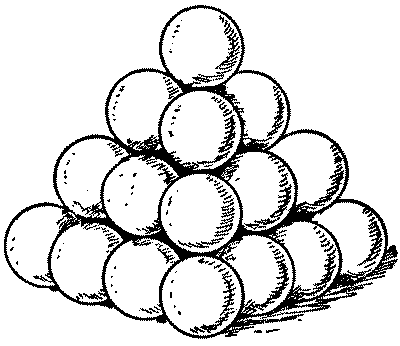
\includegraphics[height=5cm]{cannonballs}}
\pause
\only<3>{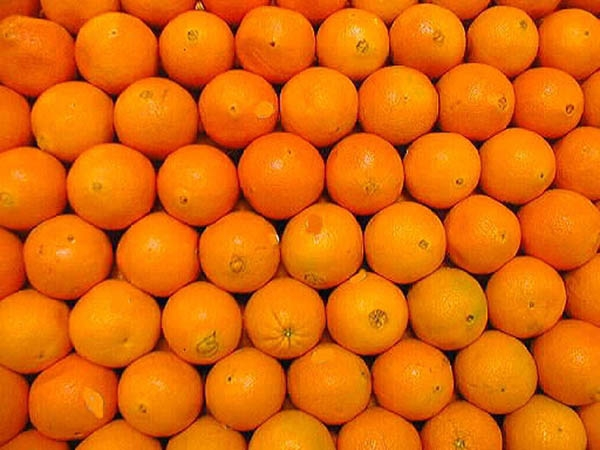
\includegraphics[height=5cm]{oranges}}
\pause
\only<4>{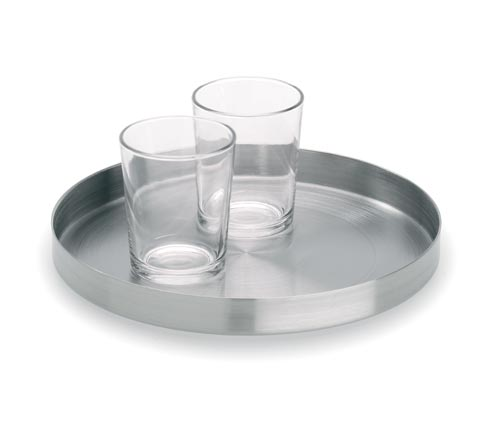
\includegraphics[height=5cm]{dienblad}}
\pause
\only<5>{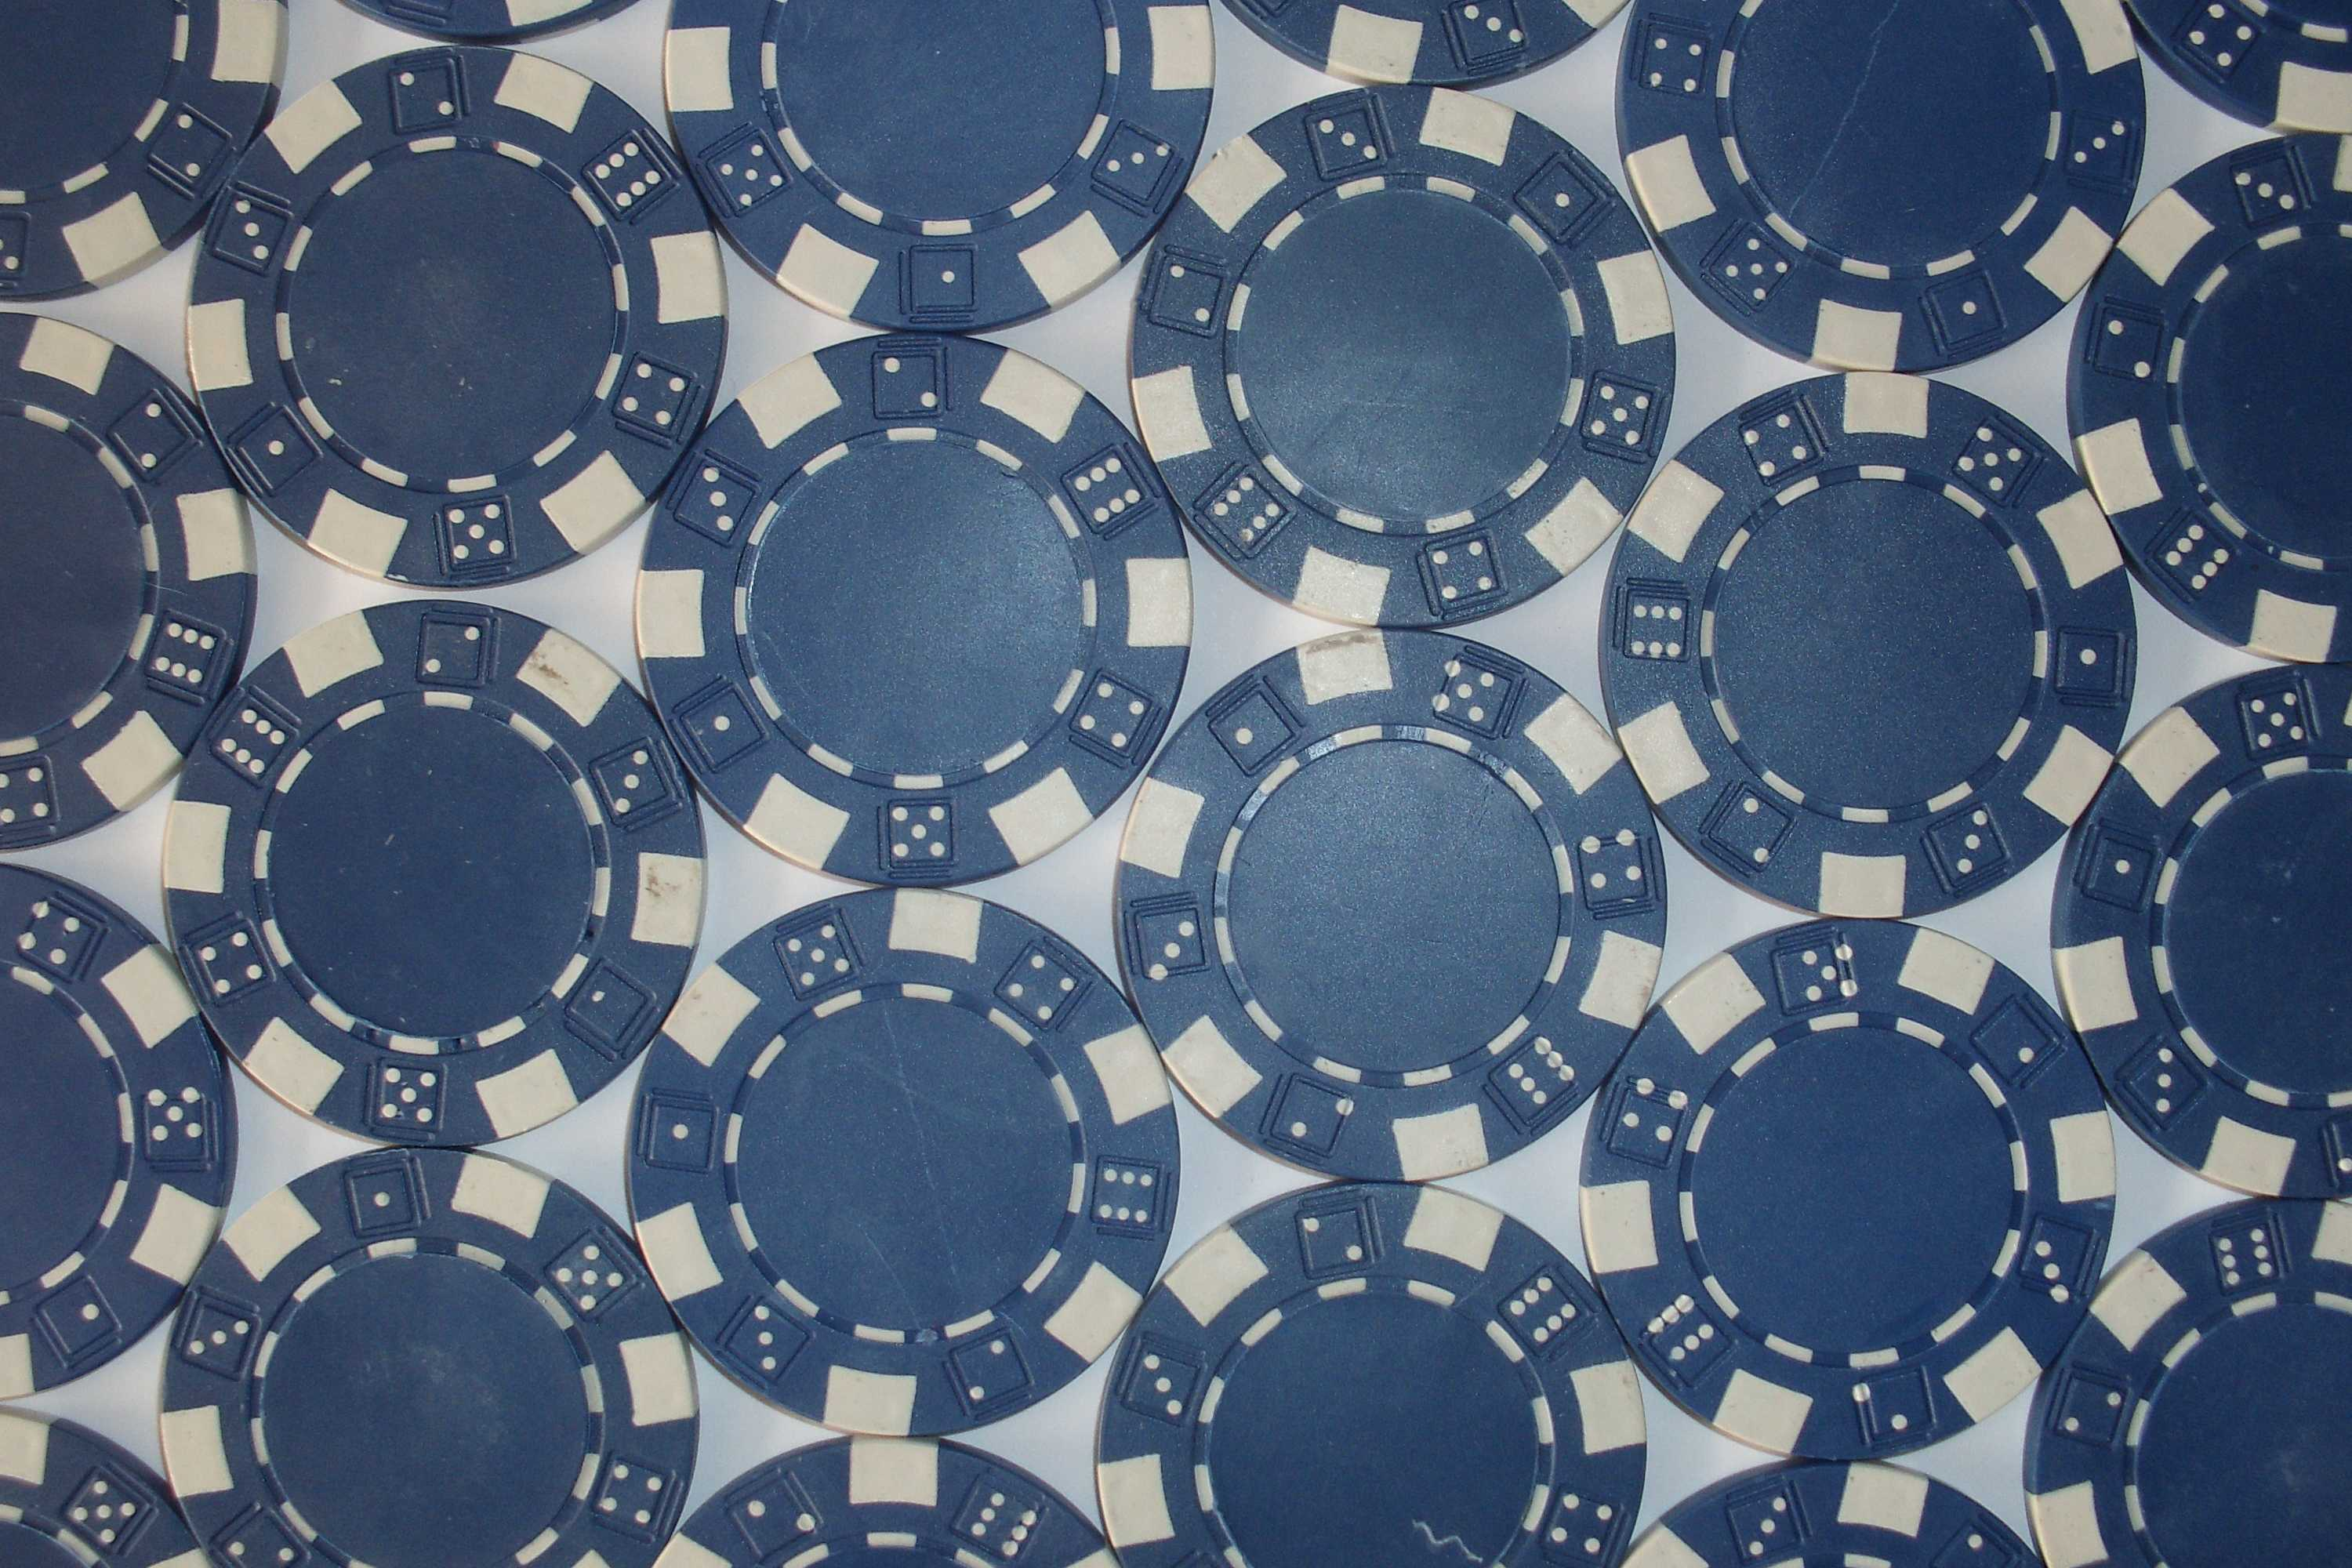
\includegraphics[height=5cm]{jetons_hex}}
\pause
\only<6>{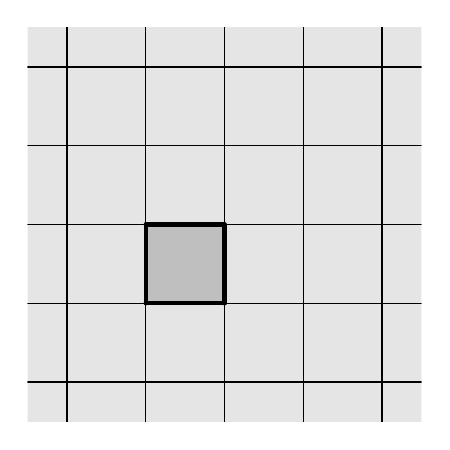
\begin{tikzpicture}[line cap=round,line join=round,>=triangle 45,x=1.0cm,y=1.0cm]
\clip(0.5,0.5) rectangle (5.5,5.5);
\fill[fill=black,fill opacity=0.1] (0,0) -- (1,0) -- (1,1) -- (0,1) -- cycle;
\fill[fill=black,fill opacity=0.1] (1,0) -- (2,0) -- (2,1) -- (1,1) -- cycle;
\fill[fill=black,fill opacity=0.1] (2,0) -- (3,0) -- (3,1) -- (2,1) -- cycle;
\fill[fill=black,fill opacity=0.1] (3,0) -- (4,0) -- (4,1) -- (3,1) -- cycle;
\fill[fill=black,fill opacity=0.1] (4,0) -- (5,0) -- (5,1) -- (4,1) -- cycle;
\fill[fill=black,fill opacity=0.1] (5,0) -- (6,0) -- (6,1) -- (5,1) -- cycle;
\fill[fill=black,fill opacity=0.1] (6,0) -- (7,0) -- (7,1) -- (6,1) -- cycle;
\fill[fill=black,fill opacity=0.1] (7,0) -- (8,0) -- (8,1) -- (7,1) -- cycle;
\fill[fill=black,fill opacity=0.1] (0,1) -- (1,1) -- (1,2) -- (0,2) -- cycle;
\fill[fill=black,fill opacity=0.1] (1,1) -- (2,1) -- (2,2) -- (1,2) -- cycle;
\fill[fill=black,fill opacity=0.1] (2,1) -- (3,1) -- (3,2) -- (2,2) -- cycle;
\fill[fill=black,fill opacity=0.1] (3,1) -- (4,1) -- (4,2) -- (3,2) -- cycle;
\fill[fill=black,fill opacity=0.1] (4,1) -- (5,1) -- (5,2) -- (4,2) -- cycle;
\fill[fill=black,fill opacity=0.1] (5,1) -- (6,1) -- (6,2) -- (5,2) -- cycle;
\fill[fill=black,fill opacity=0.1] (6,1) -- (7,1) -- (7,2) -- (6,2) -- cycle;
\fill[fill=black,fill opacity=0.1] (7,1) -- (8,1) -- (8,2) -- (7,2) -- cycle;
\fill[fill=black,fill opacity=0.1] (0,2) -- (1,2) -- (1,3) -- (0,3) -- cycle;
\fill[fill=black,fill opacity=0.1] (1,2) -- (2,2) -- (2,3) -- (1,3) -- cycle;
\fill[line width=1.6pt,fill=black,fill opacity=0.25] (2,2) -- (3,2) -- (3,3) -- (2,3) -- cycle;
\fill[fill=black,fill opacity=0.1] (3,2) -- (4,2) -- (4,3) -- (3,3) -- cycle;
\fill[fill=black,fill opacity=0.1] (4,2) -- (5,2) -- (5,3) -- (4,3) -- cycle;
\fill[fill=black,fill opacity=0.1] (5,2) -- (6,2) -- (6,3) -- (5,3) -- cycle;
\fill[fill=black,fill opacity=0.1] (6,2) -- (7,2) -- (7,3) -- (6,3) -- cycle;
\fill[fill=black,fill opacity=0.1] (7,2) -- (8,2) -- (8,3) -- (7,3) -- cycle;
\fill[fill=black,fill opacity=0.1] (0,3) -- (1,3) -- (1,4) -- (0,4) -- cycle;
\fill[fill=black,fill opacity=0.1] (1,3) -- (2,3) -- (2,4) -- (1,4) -- cycle;
\fill[fill=black,fill opacity=0.1] (2,3) -- (3,3) -- (3,4) -- (2,4) -- cycle;
\fill[fill=black,fill opacity=0.1] (3,3) -- (4,3) -- (4,4) -- (3,4) -- cycle;
\fill[fill=black,fill opacity=0.1] (4,3) -- (5,3) -- (5,4) -- (4,4) -- cycle;
\fill[fill=black,fill opacity=0.1] (5,3) -- (6,3) -- (6,4) -- (5,4) -- cycle;
\fill[fill=black,fill opacity=0.1] (6,3) -- (7,3) -- (7,4) -- (6,4) -- cycle;
\fill[fill=black,fill opacity=0.1] (7,3) -- (8,3) -- (8,4) -- (7,4) -- cycle;
\fill[fill=black,fill opacity=0.1] (0,4) -- (1,4) -- (1,5) -- (0,5) -- cycle;
\fill[fill=black,fill opacity=0.1] (1,4) -- (2,4) -- (2,5) -- (1,5) -- cycle;
\fill[fill=black,fill opacity=0.1] (2,4) -- (3,4) -- (3,5) -- (2,5) -- cycle;
\fill[fill=black,fill opacity=0.1] (3,4) -- (4,4) -- (4,5) -- (3,5) -- cycle;
\fill[fill=black,fill opacity=0.1] (4,4) -- (5,4) -- (5,5) -- (4,5) -- cycle;
\fill[fill=black,fill opacity=0.1] (5,4) -- (6,4) -- (6,5) -- (5,5) -- cycle;
\fill[fill=black,fill opacity=0.1] (6,4) -- (7,4) -- (7,5) -- (6,5) -- cycle;
\fill[fill=black,fill opacity=0.1] (7,4) -- (8,4) -- (8,5) -- (7,5) -- cycle;
\fill[fill=black,fill opacity=0.1] (0,5) -- (1,5) -- (1,6) -- (0,6) -- cycle;
\fill[fill=black,fill opacity=0.1] (1,5) -- (2,5) -- (2,6) -- (1,6) -- cycle;
\fill[fill=black,fill opacity=0.1] (2,5) -- (3,5) -- (3,6) -- (2,6) -- cycle;
\fill[fill=black,fill opacity=0.1] (3,5) -- (4,5) -- (4,6) -- (3,6) -- cycle;
\fill[fill=black,fill opacity=0.1] (4,5) -- (5,5) -- (5,6) -- (4,6) -- cycle;
\fill[fill=black,fill opacity=0.1] (5,5) -- (6,5) -- (6,6) -- (5,6) -- cycle;
\fill[fill=black,fill opacity=0.1] (6,5) -- (7,5) -- (7,6) -- (6,6) -- cycle;
\fill[fill=black,fill opacity=0.1] (7,5) -- (8,5) -- (8,6) -- (7,6) -- cycle;
\fill[fill=black,fill opacity=0.1] (0,6) -- (1,6) -- (1,7) -- (0,7) -- cycle;
\fill[fill=black,fill opacity=0.1] (1,6) -- (2,6) -- (2,7) -- (1,7) -- cycle;
\fill[fill=black,fill opacity=0.1] (2,6) -- (3,6) -- (3,7) -- (2,7) -- cycle;
\fill[fill=black,fill opacity=0.1] (3,6) -- (4,6) -- (4,7) -- (3,7) -- cycle;
\fill[fill=black,fill opacity=0.1] (4,6) -- (5,6) -- (5,7) -- (4,7) -- cycle;
\fill[fill=black,fill opacity=0.1] (5,6) -- (6,6) -- (6,7) -- (5,7) -- cycle;
\fill[fill=black,fill opacity=0.1] (6,6) -- (7,6) -- (7,7) -- (6,7) -- cycle;
\fill[fill=black,fill opacity=0.1] (7,6) -- (8,6) -- (8,7) -- (7,7) -- cycle;
\fill[fill=black,fill opacity=0.1] (0,7) -- (1,7) -- (1,8) -- (0,8) -- cycle;
\fill[fill=black,fill opacity=0.1] (1,7) -- (2,7) -- (2,8) -- (1,8) -- cycle;
\fill[fill=black,fill opacity=0.1] (2,7) -- (3,7) -- (3,8) -- (2,8) -- cycle;
\fill[fill=black,fill opacity=0.1] (3,7) -- (4,7) -- (4,8) -- (3,8) -- cycle;
\fill[fill=black,fill opacity=0.1] (4,7) -- (5,7) -- (5,8) -- (4,8) -- cycle;
\fill[fill=black,fill opacity=0.1] (5,7) -- (6,7) -- (6,8) -- (5,8) -- cycle;
\fill[fill=black,fill opacity=0.1] (6,7) -- (7,7) -- (7,8) -- (6,8) -- cycle;
\fill[fill=black,fill opacity=0.1] (7,7) -- (8,7) -- (8,8) -- (7,8) -- cycle;
\draw (0,0)-- (1,0);
\draw (1,0)-- (1,1);
\draw (1,1)-- (0,1);
\draw (0,1)-- (0,0);
\draw (1,0)-- (2,0);
\draw (2,0)-- (2,1);
\draw (2,1)-- (1,1);
\draw (1,1)-- (1,0);
\draw (2,0)-- (3,0);
\draw (3,0)-- (3,1);
\draw (3,1)-- (2,1);
\draw (2,1)-- (2,0);
\draw (3,0)-- (4,0);
\draw (4,0)-- (4,1);
\draw (4,1)-- (3,1);
\draw (3,1)-- (3,0);
\draw (4,0)-- (5,0);
\draw (5,0)-- (5,1);
\draw (5,1)-- (4,1);
\draw (4,1)-- (4,0);
\draw (5,0)-- (6,0);
\draw (6,0)-- (6,1);
\draw (6,1)-- (5,1);
\draw (5,1)-- (5,0);
\draw (6,0)-- (7,0);
\draw (7,0)-- (7,1);
\draw (7,1)-- (6,1);
\draw (6,1)-- (6,0);
\draw (7,0)-- (8,0);
\draw (8,0)-- (8,1);
\draw (8,1)-- (7,1);
\draw (7,1)-- (7,0);
\draw (0,1)-- (1,1);
\draw (1,1)-- (1,2);
\draw (1,2)-- (0,2);
\draw (0,2)-- (0,1);
\draw (1,1)-- (2,1);
\draw (2,1)-- (2,2);
\draw (2,2)-- (1,2);
\draw (1,2)-- (1,1);
\draw (2,1)-- (3,1);
\draw (3,1)-- (3,2);
\draw (3,2)-- (2,2);
\draw (2,2)-- (2,1);
\draw (3,1)-- (4,1);
\draw (4,1)-- (4,2);
\draw (4,2)-- (3,2);
\draw (3,2)-- (3,1);
\draw (4,1)-- (5,1);
\draw (5,1)-- (5,2);
\draw (5,2)-- (4,2);
\draw (4,2)-- (4,1);
\draw (5,1)-- (6,1);
\draw (6,1)-- (6,2);
\draw (6,2)-- (5,2);
\draw (5,2)-- (5,1);
\draw (6,1)-- (7,1);
\draw (7,1)-- (7,2);
\draw (7,2)-- (6,2);
\draw (6,2)-- (6,1);
\draw (7,1)-- (8,1);
\draw (8,1)-- (8,2);
\draw (8,2)-- (7,2);
\draw (7,2)-- (7,1);
\draw (0,2)-- (1,2);
\draw (1,2)-- (1,3);
\draw (1,3)-- (0,3);
\draw (0,3)-- (0,2);
\draw (1,2)-- (2,2);
\draw (2,2)-- (2,3);
\draw (2,3)-- (1,3);
\draw (1,3)-- (1,2);
\draw [line width=1.6pt] (2,2)-- (3,2);
\draw [line width=1.6pt] (3,2)-- (3,3);
\draw [line width=1.6pt] (3,3)-- (2,3);
\draw [line width=1.6pt] (2,3)-- (2,2);
\draw (3,2)-- (4,2);
\draw (4,2)-- (4,3);
\draw (4,3)-- (3,3);
\draw (3,3)-- (3,2);
\draw (4,2)-- (5,2);
\draw (5,2)-- (5,3);
\draw (5,3)-- (4,3);
\draw (4,3)-- (4,2);
\draw (5,2)-- (6,2);
\draw (6,2)-- (6,3);
\draw (6,3)-- (5,3);
\draw (5,3)-- (5,2);
\draw (6,2)-- (7,2);
\draw (7,2)-- (7,3);
\draw (7,3)-- (6,3);
\draw (6,3)-- (6,2);
\draw (7,2)-- (8,2);
\draw (8,2)-- (8,3);
\draw (8,3)-- (7,3);
\draw (7,3)-- (7,2);
\draw (0,3)-- (1,3);
\draw (1,3)-- (1,4);
\draw (1,4)-- (0,4);
\draw (0,4)-- (0,3);
\draw (1,3)-- (2,3);
\draw (2,3)-- (2,4);
\draw (2,4)-- (1,4);
\draw (1,4)-- (1,3);
\draw (2,3)-- (3,3);
\draw (3,3)-- (3,4);
\draw (3,4)-- (2,4);
\draw (2,4)-- (2,3);
\draw (3,3)-- (4,3);
\draw (4,3)-- (4,4);
\draw (4,4)-- (3,4);
\draw (3,4)-- (3,3);
\draw (4,3)-- (5,3);
\draw (5,3)-- (5,4);
\draw (5,4)-- (4,4);
\draw (4,4)-- (4,3);
\draw (5,3)-- (6,3);
\draw (6,3)-- (6,4);
\draw (6,4)-- (5,4);
\draw (5,4)-- (5,3);
\draw (6,3)-- (7,3);
\draw (7,3)-- (7,4);
\draw (7,4)-- (6,4);
\draw (6,4)-- (6,3);
\draw (7,3)-- (8,3);
\draw (8,3)-- (8,4);
\draw (8,4)-- (7,4);
\draw (7,4)-- (7,3);
\draw (0,4)-- (1,4);
\draw (1,4)-- (1,5);
\draw (1,5)-- (0,5);
\draw (0,5)-- (0,4);
\draw (1,4)-- (2,4);
\draw (2,4)-- (2,5);
\draw (2,5)-- (1,5);
\draw (1,5)-- (1,4);
\draw (2,4)-- (3,4);
\draw (3,4)-- (3,5);
\draw (3,5)-- (2,5);
\draw (2,5)-- (2,4);
\draw (3,4)-- (4,4);
\draw (4,4)-- (4,5);
\draw (4,5)-- (3,5);
\draw (3,5)-- (3,4);
\draw (4,4)-- (5,4);
\draw (5,4)-- (5,5);
\draw (5,5)-- (4,5);
\draw (4,5)-- (4,4);
\draw (5,4)-- (6,4);
\draw (6,4)-- (6,5);
\draw (6,5)-- (5,5);
\draw (5,5)-- (5,4);
\draw (6,4)-- (7,4);
\draw (7,4)-- (7,5);
\draw (7,5)-- (6,5);
\draw (6,5)-- (6,4);
\draw (7,4)-- (8,4);
\draw (8,4)-- (8,5);
\draw (8,5)-- (7,5);
\draw (7,5)-- (7,4);
\draw (0,5)-- (1,5);
\draw (1,5)-- (1,6);
\draw (1,6)-- (0,6);
\draw (0,6)-- (0,5);
\draw (1,5)-- (2,5);
\draw (2,5)-- (2,6);
\draw (2,6)-- (1,6);
\draw (1,6)-- (1,5);
\draw (2,5)-- (3,5);
\draw (3,5)-- (3,6);
\draw (3,6)-- (2,6);
\draw (2,6)-- (2,5);
\draw (3,5)-- (4,5);
\draw (4,5)-- (4,6);
\draw (4,6)-- (3,6);
\draw (3,6)-- (3,5);
\draw (4,5)-- (5,5);
\draw (5,5)-- (5,6);
\draw (5,6)-- (4,6);
\draw (4,6)-- (4,5);
\draw (5,5)-- (6,5);
\draw (6,5)-- (6,6);
\draw (6,6)-- (5,6);
\draw (5,6)-- (5,5);
\draw (6,5)-- (7,5);
\draw (7,5)-- (7,6);
\draw (7,6)-- (6,6);
\draw (6,6)-- (6,5);
\draw (7,5)-- (8,5);
\draw (8,5)-- (8,6);
\draw (8,6)-- (7,6);
\draw (7,6)-- (7,5);
\draw (0,6)-- (1,6);
\draw (1,6)-- (1,7);
\draw (1,7)-- (0,7);
\draw (0,7)-- (0,6);
\draw (1,6)-- (2,6);
\draw (2,6)-- (2,7);
\draw (2,7)-- (1,7);
\draw (1,7)-- (1,6);
\draw (2,6)-- (3,6);
\draw (3,6)-- (3,7);
\draw (3,7)-- (2,7);
\draw (2,7)-- (2,6);
\draw (3,6)-- (4,6);
\draw (4,6)-- (4,7);
\draw (4,7)-- (3,7);
\draw (3,7)-- (3,6);
\draw (4,6)-- (5,6);
\draw (5,6)-- (5,7);
\draw (5,7)-- (4,7);
\draw (4,7)-- (4,6);
\draw (5,6)-- (6,6);
\draw (6,6)-- (6,7);
\draw (6,7)-- (5,7);
\draw (5,7)-- (5,6);
\draw (6,6)-- (7,6);
\draw (7,6)-- (7,7);
\draw (7,7)-- (6,7);
\draw (6,7)-- (6,6);
\draw (7,6)-- (8,6);
\draw (8,6)-- (8,7);
\draw (8,7)-- (7,7);
\draw (7,7)-- (7,6);
\draw (0,7)-- (1,7);
\draw (1,7)-- (1,8);
\draw (1,8)-- (0,8);
\draw (0,8)-- (0,7);
\draw (1,7)-- (2,7);
\draw (2,7)-- (2,8);
\draw (2,8)-- (1,8);
\draw (1,8)-- (1,7);
\draw (2,7)-- (3,7);
\draw (3,7)-- (3,8);
\draw (3,8)-- (2,8);
\draw (2,8)-- (2,7);
\draw (3,7)-- (4,7);
\draw (4,7)-- (4,8);
\draw (4,8)-- (3,8);
\draw (3,8)-- (3,7);
\draw (4,7)-- (5,7);
\draw (5,7)-- (5,8);
\draw (5,8)-- (4,8);
\draw (4,8)-- (4,7);
\draw (5,7)-- (6,7);
\draw (6,7)-- (6,8);
\draw (6,8)-- (5,8);
\draw (5,8)-- (5,7);
\draw (6,7)-- (7,7);
\draw (7,7)-- (7,8);
\draw (7,8)-- (6,8);
\draw (6,8)-- (6,7);
\draw (7,7)-- (8,7);
\draw (8,7)-- (8,8);
\draw (8,8)-- (7,8);
\draw (7,8)-- (7,7);
\end{tikzpicture}
}
\end{figure}
\end{frame}


%\subsection{Doelgroep en voorkennis}

\begin{frame}
\frametitle{Doelgroep}
\pause
\begin{itemize}
\item $2^{de}$ graad ASO
\pause
\item Ook $3^{de}$ graad \pause, maar \ldots
\end{itemize}
\end{frame}


\begin{frame}
\frametitle{Voorkennis}
\pause
\begin{itemize}
\item verschillende vakgebieden
\pause
\begin{itemize}
\item getallenleer en algebra
\item re\"{e}le functies
\item meetkunde
\end{itemize}
\pause
\item `voorkennis'
\end{itemize}
\end{frame}

\section{Lessenreeks}

\begin{frame}
\begin{block}{
\begin{center}
\Large{Vullen van Vlakken en Volumes}
\end{center}}
\end{block}
\end{frame}

\subsection{Les 1: Inleiding}
\begin{frame}
\frametitle{Les 1: Inleiding}
\framesubtitle{Overzicht van de lessen}
\begin{list}{\quad}{}
\item {\color{blue}Les 1: Inleiding}
\item Les 2: Vullen van vierkanten met kleinere vierkanten en zo tot Perfecte Vierkanten komen
\item Les 3: Puzzelen met vierkanten en rechthoeken om vergelijkingen op te lossen
\item Les 4: Kennismaking met tweedimensionale stapelproblemen en het dienbladenprobleem 
\item Les 5: Het dienbladenprobleem: experimenteren en effectief berekenen
\item Les 6: Het dienbladenprobleem: berekenen, bewijzen en besluiten
\item Les 7: Kanonskogels stapelen
\item Les 8: Vervolg kanonskogels en het bolstapelprobleem van Kepler
\end{list}
\end{frame}

\begin{frame}
\frametitle{Les 1: Inleiding}
\framesubtitle{Lesdoelstellingen}
\begin{itemize}
\item De leerlingen kennen de definities van een \textbf{vlakvulling}, een \textbf{complete vlakvulling} en een \textbf{optimale vlakvullling}.
\item De leerlingen kunnen in groep komen tot bevindingen over het \textbf{compleet vullen} van een \textbf{oneindig groot vlak}.
\item De leerlingen kunnen bewijzen dat een \textbf{betegeling} van een oneindig groot vlak \textbf{met regelmatige veelhoeken} enkel lukt met regelmatige driehoeken, regelmatige vierhoeken en regelmatige zeshoeken.
\item De leerlingen kennen \textbf{stapelproblemen}.
\item De leerlingen kunnen \textbf{zelfstandig} op zoek gaan naar meer informatie over het lesonderwerp.
\item De leerlingen kunnen \textbf{in groep samenwerken} om enkele raadsels en puzzels op te lossen.
\end{itemize}
\end{frame}

\begin{frame}
\frametitle{Les 1: Inleiding}
\framesubtitle{Didactische wenken}
\begin{enumerate}
	\item Onderwijsleergesprek / klasgesprek
	\begin{itemize}
	\item Kennismaking met definities
	\end{itemize}
	\item Groepswerk
	\begin{itemize}
	\item Regelmatige veelhoeken in karton uitgeknipt
	\item Experimenteren
	\item Bewijs
	\end{itemize}
  \item Onderwijsleergesprek
  \begin{itemize}
	\item Kennismaking met definities
	\end{itemize}
	\item Groepswerk
	\begin{itemize}
	\item Zelfstandig informatie opzoeken
	\item Raadsels en puzzels oplossen
	\end{itemize}
\end{enumerate}
\end{frame}

\begin{frame}
\frametitle{Vullen van vlakken}
\begin{columns}
        \begin{column}{0.4\textwidth}
        \only<1-2>{Een \textbf{vlakvulling} is een vulling van het vlak met figuren, waarbij er geen gaten mogen zijn en de figuren niet mogen overlappen.}
        \only<3>{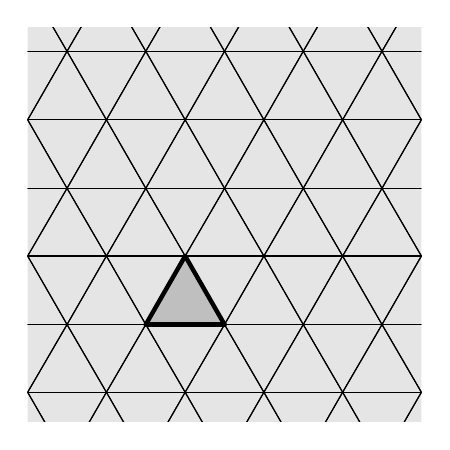
\begin{tikzpicture}[line cap=round,line join=round,>=triangle 45,x=1.0cm,y=1.0cm]
\clip(0.5,0.5) rectangle (5.5,5.5);
\fill[fill=black,fill opacity=0.1] (0,0) -- (1,0) -- (0.5,0.87) -- cycle;
\fill[fill=black,fill opacity=0.1] (0.5,0.87) -- (1,0) -- (1.5,0.87) -- cycle;
\fill[fill=black,fill opacity=0.1] (1,0) -- (2,0) -- (1.5,0.87) -- cycle;
\fill[fill=black,fill opacity=0.1] (1.5,0.87) -- (2,0) -- (2.5,0.87) -- cycle;
\fill[fill=black,fill opacity=0.1] (2,0) -- (3,0) -- (2.5,0.87) -- cycle;
\fill[fill=black,fill opacity=0.1] (2.5,0.87) -- (3,0) -- (3.5,0.87) -- cycle;
\fill[fill=black,fill opacity=0.1] (3,0) -- (4,0) -- (3.5,0.87) -- cycle;
\fill[fill=black,fill opacity=0.1] (3.5,0.87) -- (4,0) -- (4.5,0.87) -- cycle;
\fill[fill=black,fill opacity=0.1] (4,0) -- (5,0) -- (4.5,0.87) -- cycle;
\fill[fill=black,fill opacity=0.1] (4.5,0.87) -- (5,0) -- (5.5,0.87) -- cycle;
\fill[fill=black,fill opacity=0.1] (5,0) -- (6,0) -- (5.5,0.87) -- cycle;
\fill[fill=black,fill opacity=0.1] (5.5,0.87) -- (6,0) -- (6.5,0.87) -- cycle;
\fill[fill=black,fill opacity=0.1] (6,0) -- (7,0) -- (6.5,0.87) -- cycle;
\fill[fill=black,fill opacity=0.1] (6.5,0.87) -- (7,0) -- (7.5,0.87) -- cycle;
\fill[fill=black,fill opacity=0.1] (7,0) -- (8,0) -- (7.5,0.87) -- cycle;
\fill[fill=black,fill opacity=0.1] (7.5,0.87) -- (8,0) -- (8.5,0.87) -- cycle;
\fill[fill=black,fill opacity=0.1] (8,0) -- (9,0) -- (8.5,0.87) -- cycle;
\fill[fill=black,fill opacity=0.1] (8.5,0.87) -- (9,0) -- (9.5,0.87) -- cycle;
\fill[fill=black,fill opacity=0.1] (9,0) -- (10,0) -- (9.5,0.87) -- cycle;
\fill[fill=black,fill opacity=0.1] (9.5,0.87) -- (10,0) -- (10.5,0.87) -- cycle;
\fill[fill=black,fill opacity=0.1] (0,1.73) -- (0.5,0.87) -- (1,1.73) -- cycle;
\fill[fill=black,fill opacity=0.1] (0.5,0.87) -- (1.5,0.87) -- (1,1.73) -- cycle;
\fill[fill=black,fill opacity=0.1] (1,1.73) -- (1.5,0.87) -- (2,1.73) -- cycle;
\fill[fill=black,fill opacity=0.1] (1.5,0.87) -- (2.5,0.87) -- (2,1.73) -- cycle;
\fill[fill=black,fill opacity=0.1] (2,1.73) -- (2.5,0.87) -- (3,1.73) -- cycle;
\fill[fill=black,fill opacity=0.1] (2.5,0.87) -- (3.5,0.87) -- (3,1.73) -- cycle;
\fill[fill=black,fill opacity=0.1] (3,1.73) -- (3.5,0.87) -- (4,1.73) -- cycle;
\fill[fill=black,fill opacity=0.1] (3.5,0.87) -- (4.5,0.87) -- (4,1.73) -- cycle;
\fill[fill=black,fill opacity=0.1] (4,1.73) -- (4.5,0.87) -- (5,1.73) -- cycle;
\fill[fill=black,fill opacity=0.1] (4.5,0.87) -- (5.5,0.87) -- (5,1.73) -- cycle;
\fill[fill=black,fill opacity=0.1] (5,1.73) -- (5.5,0.87) -- (6,1.73) -- cycle;
\fill[fill=black,fill opacity=0.1] (5.5,0.87) -- (6.5,0.87) -- (6,1.73) -- cycle;
\fill[fill=black,fill opacity=0.1] (6,1.73) -- (6.5,0.87) -- (7,1.73) -- cycle;
\fill[fill=black,fill opacity=0.1] (6.5,0.87) -- (7.5,0.87) -- (7,1.73) -- cycle;
\fill[fill=black,fill opacity=0.1] (7,1.73) -- (7.5,0.87) -- (8,1.73) -- cycle;
\fill[fill=black,fill opacity=0.1] (7.5,0.87) -- (8.5,0.87) -- (8,1.73) -- cycle;
\fill[fill=black,fill opacity=0.1] (8,1.73) -- (8.5,0.87) -- (9,1.73) -- cycle;
\fill[fill=black,fill opacity=0.1] (8.5,0.87) -- (9.5,0.87) -- (9,1.73) -- cycle;
\fill[fill=black,fill opacity=0.1] (9,1.73) -- (9.5,0.87) -- (10,1.73) -- cycle;
\fill[fill=black,fill opacity=0.1] (9.5,0.87) -- (10.5,0.87) -- (10,1.73) -- cycle;
\fill[fill=black,fill opacity=0.1] (0,1.73) -- (1,1.73) -- (0.5,2.6) -- cycle;
\fill[fill=black,fill opacity=0.1] (0.5,2.6) -- (1,1.73) -- (1.5,2.6) -- cycle;
\fill[fill=black,fill opacity=0.1] (1,1.73) -- (2,1.73) -- (1.5,2.6) -- cycle;
\fill[fill=black,fill opacity=0.1] (1.5,2.6) -- (2,1.73) -- (2.5,2.6) -- cycle;
\fill[line width=1.6pt,fill=black,fill opacity=0.25] (2,1.73) -- (3,1.73) -- (2.5,2.6) -- cycle;
\fill[fill=black,fill opacity=0.1] (2.5,2.6) -- (3,1.73) -- (3.5,2.6) -- cycle;
\fill[fill=black,fill opacity=0.1] (3,1.73) -- (4,1.73) -- (3.5,2.6) -- cycle;
\fill[fill=black,fill opacity=0.1] (3.5,2.6) -- (4,1.73) -- (4.5,2.6) -- cycle;
\fill[fill=black,fill opacity=0.1] (4,1.73) -- (5,1.73) -- (4.5,2.6) -- cycle;
\fill[fill=black,fill opacity=0.1] (4.5,2.6) -- (5,1.73) -- (5.5,2.6) -- cycle;
\fill[fill=black,fill opacity=0.1] (5,1.73) -- (6,1.73) -- (5.5,2.6) -- cycle;
\fill[fill=black,fill opacity=0.1] (5.5,2.6) -- (6,1.73) -- (6.5,2.6) -- cycle;
\fill[fill=black,fill opacity=0.1] (6,1.73) -- (7,1.73) -- (6.5,2.6) -- cycle;
\fill[fill=black,fill opacity=0.1] (6.5,2.6) -- (7,1.73) -- (7.5,2.6) -- cycle;
\fill[fill=black,fill opacity=0.1] (7,1.73) -- (8,1.73) -- (7.5,2.6) -- cycle;
\fill[fill=black,fill opacity=0.1] (7.5,2.6) -- (8,1.73) -- (8.5,2.6) -- cycle;
\fill[fill=black,fill opacity=0.1] (8,1.73) -- (9,1.73) -- (8.5,2.6) -- cycle;
\fill[fill=black,fill opacity=0.1] (8.5,2.6) -- (9,1.73) -- (9.5,2.6) -- cycle;
\fill[fill=black,fill opacity=0.1] (9,1.73) -- (10,1.73) -- (9.5,2.6) -- cycle;
\fill[fill=black,fill opacity=0.1] (9.5,2.6) -- (10,1.73) -- (10.5,2.6) -- cycle;
\fill[fill=black,fill opacity=0.1] (0,3.46) -- (0.5,2.6) -- (1,3.46) -- cycle;
\fill[fill=black,fill opacity=0.1] (0.5,2.6) -- (1.5,2.6) -- (1,3.46) -- cycle;
\fill[fill=black,fill opacity=0.1] (1,3.46) -- (1.5,2.6) -- (2,3.46) -- cycle;
\fill[fill=black,fill opacity=0.1] (1.5,2.6) -- (2.5,2.6) -- (2,3.46) -- cycle;
\fill[fill=black,fill opacity=0.1] (2,3.46) -- (2.5,2.6) -- (3,3.46) -- cycle;
\fill[fill=black,fill opacity=0.1] (2.5,2.6) -- (3.5,2.6) -- (3,3.46) -- cycle;
\fill[fill=black,fill opacity=0.1] (3,3.46) -- (3.5,2.6) -- (4,3.46) -- cycle;
\fill[fill=black,fill opacity=0.1] (3.5,2.6) -- (4.5,2.6) -- (4,3.46) -- cycle;
\fill[fill=black,fill opacity=0.1] (4,3.46) -- (4.5,2.6) -- (5,3.46) -- cycle;
\fill[fill=black,fill opacity=0.1] (4.5,2.6) -- (5.5,2.6) -- (5,3.46) -- cycle;
\fill[fill=black,fill opacity=0.1] (5,3.46) -- (5.5,2.6) -- (6,3.46) -- cycle;
\fill[fill=black,fill opacity=0.1] (5.5,2.6) -- (6.5,2.6) -- (6,3.46) -- cycle;
\fill[fill=black,fill opacity=0.1] (6,3.46) -- (6.5,2.6) -- (7,3.46) -- cycle;
\fill[fill=black,fill opacity=0.1] (6.5,2.6) -- (7.5,2.6) -- (7,3.46) -- cycle;
\fill[fill=black,fill opacity=0.1] (7,3.46) -- (7.5,2.6) -- (8,3.46) -- cycle;
\fill[fill=black,fill opacity=0.1] (7.5,2.6) -- (8.5,2.6) -- (8,3.46) -- cycle;
\fill[fill=black,fill opacity=0.1] (8,3.46) -- (8.5,2.6) -- (9,3.46) -- cycle;
\fill[fill=black,fill opacity=0.1] (8.5,2.6) -- (9.5,2.6) -- (9,3.46) -- cycle;
\fill[fill=black,fill opacity=0.1] (9,3.46) -- (9.5,2.6) -- (10,3.46) -- cycle;
\fill[fill=black,fill opacity=0.1] (9.5,2.6) -- (10.5,2.6) -- (10,3.46) -- cycle;
\fill[fill=black,fill opacity=0.1] (0,3.46) -- (1,3.46) -- (0.5,4.33) -- cycle;
\fill[fill=black,fill opacity=0.1] (0.5,4.33) -- (1,3.46) -- (1.5,4.33) -- cycle;
\fill[fill=black,fill opacity=0.1] (1,3.46) -- (2,3.46) -- (1.5,4.33) -- cycle;
\fill[fill=black,fill opacity=0.1] (1.5,4.33) -- (2,3.46) -- (2.5,4.33) -- cycle;
\fill[fill=black,fill opacity=0.1] (2,3.46) -- (3,3.46) -- (2.5,4.33) -- cycle;
\fill[fill=black,fill opacity=0.1] (2.5,4.33) -- (3,3.46) -- (3.5,4.33) -- cycle;
\fill[fill=black,fill opacity=0.1] (3,3.46) -- (4,3.46) -- (3.5,4.33) -- cycle;
\fill[fill=black,fill opacity=0.1] (3.5,4.33) -- (4,3.46) -- (4.5,4.33) -- cycle;
\fill[fill=black,fill opacity=0.1] (4,3.46) -- (5,3.46) -- (4.5,4.33) -- cycle;
\fill[fill=black,fill opacity=0.1] (4.5,4.33) -- (5,3.46) -- (5.5,4.33) -- cycle;
\fill[fill=black,fill opacity=0.1] (5,3.46) -- (6,3.46) -- (5.5,4.33) -- cycle;
\fill[fill=black,fill opacity=0.1] (5.5,4.33) -- (6,3.46) -- (6.5,4.33) -- cycle;
\fill[fill=black,fill opacity=0.1] (6,3.46) -- (7,3.46) -- (6.5,4.33) -- cycle;
\fill[fill=black,fill opacity=0.1] (6.5,4.33) -- (7,3.46) -- (7.5,4.33) -- cycle;
\fill[fill=black,fill opacity=0.1] (7,3.46) -- (8,3.46) -- (7.5,4.33) -- cycle;
\fill[fill=black,fill opacity=0.1] (7.5,4.33) -- (8,3.46) -- (8.5,4.33) -- cycle;
\fill[fill=black,fill opacity=0.1] (8,3.46) -- (9,3.46) -- (8.5,4.33) -- cycle;
\fill[fill=black,fill opacity=0.1] (8.5,4.33) -- (9,3.46) -- (9.5,4.33) -- cycle;
\fill[fill=black,fill opacity=0.1] (9,3.46) -- (10,3.46) -- (9.5,4.33) -- cycle;
\fill[fill=black,fill opacity=0.1] (9.5,4.33) -- (10,3.46) -- (10.5,4.33) -- cycle;
\fill[fill=black,fill opacity=0.1] (0,5.2) -- (0.5,4.33) -- (1,5.2) -- cycle;
\fill[fill=black,fill opacity=0.1] (0.5,4.33) -- (1.5,4.33) -- (1,5.2) -- cycle;
\fill[fill=black,fill opacity=0.1] (1,5.2) -- (1.5,4.33) -- (2,5.2) -- cycle;
\fill[fill=black,fill opacity=0.1] (1.5,4.33) -- (2.5,4.33) -- (2,5.2) -- cycle;
\fill[fill=black,fill opacity=0.1] (2,5.2) -- (2.5,4.33) -- (3,5.2) -- cycle;
\fill[fill=black,fill opacity=0.1] (2.5,4.33) -- (3.5,4.33) -- (3,5.2) -- cycle;
\fill[fill=black,fill opacity=0.1] (3,5.2) -- (3.5,4.33) -- (4,5.2) -- cycle;
\fill[fill=black,fill opacity=0.1] (3.5,4.33) -- (4.5,4.33) -- (4,5.2) -- cycle;
\fill[fill=black,fill opacity=0.1] (4,5.2) -- (4.5,4.33) -- (5,5.2) -- cycle;
\fill[fill=black,fill opacity=0.1] (4.5,4.33) -- (5.5,4.33) -- (5,5.2) -- cycle;
\fill[fill=black,fill opacity=0.1] (5,5.2) -- (5.5,4.33) -- (6,5.2) -- cycle;
\fill[fill=black,fill opacity=0.1] (5.5,4.33) -- (6.5,4.33) -- (6,5.2) -- cycle;
\fill[fill=black,fill opacity=0.1] (6,5.2) -- (6.5,4.33) -- (7,5.2) -- cycle;
\fill[fill=black,fill opacity=0.1] (6.5,4.33) -- (7.5,4.33) -- (7,5.2) -- cycle;
\fill[fill=black,fill opacity=0.1] (7,5.2) -- (7.5,4.33) -- (8,5.2) -- cycle;
\fill[fill=black,fill opacity=0.1] (7.5,4.33) -- (8.5,4.33) -- (8,5.2) -- cycle;
\fill[fill=black,fill opacity=0.1] (8,5.2) -- (8.5,4.33) -- (9,5.2) -- cycle;
\fill[fill=black,fill opacity=0.1] (8.5,4.33) -- (9.5,4.33) -- (9,5.2) -- cycle;
\fill[fill=black,fill opacity=0.1] (9,5.2) -- (9.5,4.33) -- (10,5.2) -- cycle;
\fill[fill=black,fill opacity=0.1] (9.5,4.33) -- (10.5,4.33) -- (10,5.2) -- cycle;
\fill[fill=black,fill opacity=0.1] (0,5.2) -- (1,5.2) -- (0.5,6.06) -- cycle;
\fill[fill=black,fill opacity=0.1] (0.5,6.06) -- (1,5.2) -- (1.5,6.06) -- cycle;
\fill[fill=black,fill opacity=0.1] (1,5.2) -- (2,5.2) -- (1.5,6.06) -- cycle;
\fill[fill=black,fill opacity=0.1] (1.5,6.06) -- (2,5.2) -- (2.5,6.06) -- cycle;
\fill[fill=black,fill opacity=0.1] (2,5.2) -- (3,5.2) -- (2.5,6.06) -- cycle;
\fill[fill=black,fill opacity=0.1] (2.5,6.06) -- (3,5.2) -- (3.5,6.06) -- cycle;
\fill[fill=black,fill opacity=0.1] (3,5.2) -- (4,5.2) -- (3.5,6.06) -- cycle;
\fill[fill=black,fill opacity=0.1] (3.5,6.06) -- (4,5.2) -- (4.5,6.06) -- cycle;
\fill[fill=black,fill opacity=0.1] (4,5.2) -- (5,5.2) -- (4.5,6.06) -- cycle;
\fill[fill=black,fill opacity=0.1] (4.5,6.06) -- (5,5.2) -- (5.5,6.06) -- cycle;
\fill[fill=black,fill opacity=0.1] (5,5.2) -- (6,5.2) -- (5.5,6.06) -- cycle;
\fill[fill=black,fill opacity=0.1] (5.5,6.06) -- (6,5.2) -- (6.5,6.06) -- cycle;
\fill[fill=black,fill opacity=0.1] (6,5.2) -- (7,5.2) -- (6.5,6.06) -- cycle;
\fill[fill=black,fill opacity=0.1] (6.5,6.06) -- (7,5.2) -- (7.5,6.06) -- cycle;
\fill[fill=black,fill opacity=0.1] (7,5.2) -- (8,5.2) -- (7.5,6.06) -- cycle;
\fill[fill=black,fill opacity=0.1] (7.5,6.06) -- (8,5.2) -- (8.5,6.06) -- cycle;
\fill[fill=black,fill opacity=0.1] (8,5.2) -- (9,5.2) -- (8.5,6.06) -- cycle;
\fill[fill=black,fill opacity=0.1] (8.5,6.06) -- (9,5.2) -- (9.5,6.06) -- cycle;
\fill[fill=black,fill opacity=0.1] (9,5.2) -- (10,5.2) -- (9.5,6.06) -- cycle;
\fill[fill=black,fill opacity=0.1] (9.5,6.06) -- (10,5.2) -- (10.5,6.06) -- cycle;
\fill[fill=black,fill opacity=0.1] (0,6.93) -- (0.5,6.06) -- (1,6.93) -- cycle;
\fill[fill=black,fill opacity=0.1] (0.5,6.06) -- (1.5,6.06) -- (1,6.93) -- cycle;
\fill[fill=black,fill opacity=0.1] (1,6.93) -- (1.5,6.06) -- (2,6.93) -- cycle;
\fill[fill=black,fill opacity=0.1] (1.5,6.06) -- (2.5,6.06) -- (2,6.93) -- cycle;
\fill[fill=black,fill opacity=0.1] (2,6.93) -- (2.5,6.06) -- (3,6.93) -- cycle;
\fill[fill=black,fill opacity=0.1] (2.5,6.06) -- (3.5,6.06) -- (3,6.93) -- cycle;
\fill[fill=black,fill opacity=0.1] (3,6.93) -- (3.5,6.06) -- (4,6.93) -- cycle;
\fill[fill=black,fill opacity=0.1] (3.5,6.06) -- (4.5,6.06) -- (4,6.93) -- cycle;
\fill[fill=black,fill opacity=0.1] (4,6.93) -- (4.5,6.06) -- (5,6.93) -- cycle;
\fill[fill=black,fill opacity=0.1] (4.5,6.06) -- (5.5,6.06) -- (5,6.93) -- cycle;
\fill[fill=black,fill opacity=0.1] (5,6.93) -- (5.5,6.06) -- (6,6.93) -- cycle;
\fill[fill=black,fill opacity=0.1] (5.5,6.06) -- (6.5,6.06) -- (6,6.93) -- cycle;
\fill[fill=black,fill opacity=0.1] (6,6.93) -- (6.5,6.06) -- (7,6.93) -- cycle;
\fill[fill=black,fill opacity=0.1] (6.5,6.06) -- (7.5,6.06) -- (7,6.93) -- cycle;
\fill[fill=black,fill opacity=0.1] (7,6.93) -- (7.5,6.06) -- (8,6.93) -- cycle;
\fill[fill=black,fill opacity=0.1] (7.5,6.06) -- (8.5,6.06) -- (8,6.93) -- cycle;
\fill[fill=black,fill opacity=0.1] (8,6.93) -- (8.5,6.06) -- (9,6.93) -- cycle;
\fill[fill=black,fill opacity=0.1] (8.5,6.06) -- (9.5,6.06) -- (9,6.93) -- cycle;
\fill[fill=black,fill opacity=0.1] (9,6.93) -- (9.5,6.06) -- (10,6.93) -- cycle;
\fill[fill=black,fill opacity=0.1] (9.5,6.06) -- (10.5,6.06) -- (10,6.93) -- cycle;
\fill[fill=black,fill opacity=0.1] (0,6.93) -- (1,6.93) -- (0.5,7.79) -- cycle;
\fill[fill=black,fill opacity=0.1] (0.5,7.79) -- (1,6.93) -- (1.5,7.79) -- cycle;
\fill[fill=black,fill opacity=0.1] (1,6.93) -- (2,6.93) -- (1.5,7.79) -- cycle;
\fill[fill=black,fill opacity=0.1] (1.5,7.79) -- (2,6.93) -- (2.5,7.79) -- cycle;
\fill[fill=black,fill opacity=0.1] (2,6.93) -- (3,6.93) -- (2.5,7.79) -- cycle;
\fill[fill=black,fill opacity=0.1] (2.5,7.79) -- (3,6.93) -- (3.5,7.79) -- cycle;
\fill[fill=black,fill opacity=0.1] (3,6.93) -- (4,6.93) -- (3.5,7.79) -- cycle;
\fill[fill=black,fill opacity=0.1] (3.5,7.79) -- (4,6.93) -- (4.5,7.79) -- cycle;
\fill[fill=black,fill opacity=0.1] (4,6.93) -- (5,6.93) -- (4.5,7.79) -- cycle;
\fill[fill=black,fill opacity=0.1] (4.5,7.79) -- (5,6.93) -- (5.5,7.79) -- cycle;
\fill[fill=black,fill opacity=0.1] (5,6.93) -- (6,6.93) -- (5.5,7.79) -- cycle;
\fill[fill=black,fill opacity=0.1] (5.5,7.79) -- (6,6.93) -- (6.5,7.79) -- cycle;
\fill[fill=black,fill opacity=0.1] (6,6.93) -- (7,6.93) -- (6.5,7.79) -- cycle;
\fill[fill=black,fill opacity=0.1] (6.5,7.79) -- (7,6.93) -- (7.5,7.79) -- cycle;
\fill[fill=black,fill opacity=0.1] (7,6.93) -- (8,6.93) -- (7.5,7.79) -- cycle;
\fill[fill=black,fill opacity=0.1] (7.5,7.79) -- (8,6.93) -- (8.5,7.79) -- cycle;
\fill[fill=black,fill opacity=0.1] (8,6.93) -- (9,6.93) -- (8.5,7.79) -- cycle;
\fill[fill=black,fill opacity=0.1] (8.5,7.79) -- (9,6.93) -- (9.5,7.79) -- cycle;
\fill[fill=black,fill opacity=0.1] (9,6.93) -- (10,6.93) -- (9.5,7.79) -- cycle;
\fill[fill=black,fill opacity=0.1] (9.5,7.79) -- (10,6.93) -- (10.5,7.79) -- cycle;
\fill[fill=black,fill opacity=0.1] (0,8.66) -- (0.5,7.79) -- (1,8.66) -- cycle;
\fill[fill=black,fill opacity=0.1] (0.5,7.79) -- (1.5,7.79) -- (1,8.66) -- cycle;
\fill[fill=black,fill opacity=0.1] (1,8.66) -- (1.5,7.79) -- (2,8.66) -- cycle;
\fill[fill=black,fill opacity=0.1] (1.5,7.79) -- (2.5,7.79) -- (2,8.66) -- cycle;
\fill[fill=black,fill opacity=0.1] (2,8.66) -- (2.5,7.79) -- (3,8.66) -- cycle;
\fill[fill=black,fill opacity=0.1] (2.5,7.79) -- (3.5,7.79) -- (3,8.66) -- cycle;
\fill[fill=black,fill opacity=0.1] (3,8.66) -- (3.5,7.79) -- (4,8.66) -- cycle;
\fill[fill=black,fill opacity=0.1] (3.5,7.79) -- (4.5,7.79) -- (4,8.66) -- cycle;
\fill[fill=black,fill opacity=0.1] (4,8.66) -- (4.5,7.79) -- (5,8.66) -- cycle;
\fill[fill=black,fill opacity=0.1] (4.5,7.79) -- (5.5,7.79) -- (5,8.66) -- cycle;
\fill[fill=black,fill opacity=0.1] (5,8.66) -- (5.5,7.79) -- (6,8.66) -- cycle;
\fill[fill=black,fill opacity=0.1] (5.5,7.79) -- (6.5,7.79) -- (6,8.66) -- cycle;
\fill[fill=black,fill opacity=0.1] (6,8.66) -- (6.5,7.79) -- (7,8.66) -- cycle;
\fill[fill=black,fill opacity=0.1] (6.5,7.79) -- (7.5,7.79) -- (7,8.66) -- cycle;
\fill[fill=black,fill opacity=0.1] (7,8.66) -- (7.5,7.79) -- (8,8.66) -- cycle;
\fill[fill=black,fill opacity=0.1] (7.5,7.79) -- (8.5,7.79) -- (8,8.66) -- cycle;
\fill[fill=black,fill opacity=0.1] (8,8.66) -- (8.5,7.79) -- (9,8.66) -- cycle;
\fill[fill=black,fill opacity=0.1] (8.5,7.79) -- (9.5,7.79) -- (9,8.66) -- cycle;
\fill[fill=black,fill opacity=0.1] (9,8.66) -- (9.5,7.79) -- (10,8.66) -- cycle;
\fill[fill=black,fill opacity=0.1] (9.5,7.79) -- (10.5,7.79) -- (10,8.66) -- cycle;
\fill[fill=black,fill opacity=0.1] (0,8.66) -- (1,8.66) -- (0.5,9.53) -- cycle;
\fill[fill=black,fill opacity=0.1] (0.5,9.53) -- (1,8.66) -- (1.5,9.53) -- cycle;
\fill[fill=black,fill opacity=0.1] (1,8.66) -- (2,8.66) -- (1.5,9.53) -- cycle;
\fill[fill=black,fill opacity=0.1] (1.5,9.53) -- (2,8.66) -- (2.5,9.53) -- cycle;
\fill[fill=black,fill opacity=0.1] (2,8.66) -- (3,8.66) -- (2.5,9.53) -- cycle;
\fill[fill=black,fill opacity=0.1] (2.5,9.53) -- (3,8.66) -- (3.5,9.53) -- cycle;
\fill[fill=black,fill opacity=0.1] (3,8.66) -- (4,8.66) -- (3.5,9.53) -- cycle;
\fill[fill=black,fill opacity=0.1] (3.5,9.53) -- (4,8.66) -- (4.5,9.53) -- cycle;
\fill[fill=black,fill opacity=0.1] (4,8.66) -- (5,8.66) -- (4.5,9.53) -- cycle;
\fill[fill=black,fill opacity=0.1] (4.5,9.53) -- (5,8.66) -- (5.5,9.53) -- cycle;
\fill[fill=black,fill opacity=0.1] (5,8.66) -- (6,8.66) -- (5.5,9.53) -- cycle;
\fill[fill=black,fill opacity=0.1] (5.5,9.53) -- (6,8.66) -- (6.5,9.53) -- cycle;
\fill[fill=black,fill opacity=0.1] (6,8.66) -- (7,8.66) -- (6.5,9.53) -- cycle;
\fill[fill=black,fill opacity=0.1] (6.5,9.53) -- (7,8.66) -- (7.5,9.53) -- cycle;
\fill[fill=black,fill opacity=0.1] (7,8.66) -- (8,8.66) -- (7.5,9.53) -- cycle;
\fill[fill=black,fill opacity=0.1] (7.5,9.53) -- (8,8.66) -- (8.5,9.53) -- cycle;
\fill[fill=black,fill opacity=0.1] (8,8.66) -- (9,8.66) -- (8.5,9.53) -- cycle;
\fill[fill=black,fill opacity=0.1] (8.5,9.53) -- (9,8.66) -- (9.5,9.53) -- cycle;
\fill[fill=black,fill opacity=0.1] (9,8.66) -- (10,8.66) -- (9.5,9.53) -- cycle;
\fill[fill=black,fill opacity=0.1] (9.5,9.53) -- (10,8.66) -- (10.5,9.53) -- cycle;
\fill[fill=black,fill opacity=0.1] (0,10.39) -- (0.5,9.53) -- (1,10.39) -- cycle;
\fill[fill=black,fill opacity=0.1] (0.5,9.53) -- (1.5,9.53) -- (1,10.39) -- cycle;
\fill[fill=black,fill opacity=0.1] (1,10.39) -- (1.5,9.53) -- (2,10.39) -- cycle;
\fill[fill=black,fill opacity=0.1] (1.5,9.53) -- (2.5,9.53) -- (2,10.39) -- cycle;
\fill[fill=black,fill opacity=0.1] (2,10.39) -- (2.5,9.53) -- (3,10.39) -- cycle;
\fill[fill=black,fill opacity=0.1] (2.5,9.53) -- (3.5,9.53) -- (3,10.39) -- cycle;
\fill[fill=black,fill opacity=0.1] (3,10.39) -- (3.5,9.53) -- (4,10.39) -- cycle;
\fill[fill=black,fill opacity=0.1] (3.5,9.53) -- (4.5,9.53) -- (4,10.39) -- cycle;
\fill[fill=black,fill opacity=0.1] (4,10.39) -- (4.5,9.53) -- (5,10.39) -- cycle;
\fill[fill=black,fill opacity=0.1] (4.5,9.53) -- (5.5,9.53) -- (5,10.39) -- cycle;
\fill[fill=black,fill opacity=0.1] (5,10.39) -- (5.5,9.53) -- (6,10.39) -- cycle;
\fill[fill=black,fill opacity=0.1] (5.5,9.53) -- (6.5,9.53) -- (6,10.39) -- cycle;
\fill[fill=black,fill opacity=0.1] (6,10.39) -- (6.5,9.53) -- (7,10.39) -- cycle;
\fill[fill=black,fill opacity=0.1] (6.5,9.53) -- (7.5,9.53) -- (7,10.39) -- cycle;
\fill[fill=black,fill opacity=0.1] (7,10.39) -- (7.5,9.53) -- (8,10.39) -- cycle;
\fill[fill=black,fill opacity=0.1] (7.5,9.53) -- (8.5,9.53) -- (8,10.39) -- cycle;
\fill[fill=black,fill opacity=0.1] (8,10.39) -- (8.5,9.53) -- (9,10.39) -- cycle;
\fill[fill=black,fill opacity=0.1] (8.5,9.53) -- (9.5,9.53) -- (9,10.39) -- cycle;
\fill[fill=black,fill opacity=0.1] (9,10.39) -- (9.5,9.53) -- (10,10.39) -- cycle;
\fill[fill=black,fill opacity=0.1] (9.5,9.53) -- (10.5,9.53) -- (10,10.39) -- cycle;
\draw (0,0)-- (1,0);
\draw (1,0)-- (0.5,0.87);
\draw (0.5,0.87)-- (0,0);
\draw (0.5,0.87)-- (1,0);
\draw (1,0)-- (1.5,0.87);
\draw (1.5,0.87)-- (0.5,0.87);
\draw (1,0)-- (2,0);
\draw (2,0)-- (1.5,0.87);
\draw (1.5,0.87)-- (1,0);
\draw (1.5,0.87)-- (2,0);
\draw (2,0)-- (2.5,0.87);
\draw (2.5,0.87)-- (1.5,0.87);
\draw (2,0)-- (3,0);
\draw (3,0)-- (2.5,0.87);
\draw (2.5,0.87)-- (2,0);
\draw (2.5,0.87)-- (3,0);
\draw (3,0)-- (3.5,0.87);
\draw (3.5,0.87)-- (2.5,0.87);
\draw (3,0)-- (4,0);
\draw (4,0)-- (3.5,0.87);
\draw (3.5,0.87)-- (3,0);
\draw (3.5,0.87)-- (4,0);
\draw (4,0)-- (4.5,0.87);
\draw (4.5,0.87)-- (3.5,0.87);
\draw (4,0)-- (5,0);
\draw (5,0)-- (4.5,0.87);
\draw (4.5,0.87)-- (4,0);
\draw (4.5,0.87)-- (5,0);
\draw (5,0)-- (5.5,0.87);
\draw (5.5,0.87)-- (4.5,0.87);
\draw (5,0)-- (6,0);
\draw (6,0)-- (5.5,0.87);
\draw (5.5,0.87)-- (5,0);
\draw (5.5,0.87)-- (6,0);
\draw (6,0)-- (6.5,0.87);
\draw (6.5,0.87)-- (5.5,0.87);
\draw (6,0)-- (7,0);
\draw (7,0)-- (6.5,0.87);
\draw (6.5,0.87)-- (6,0);
\draw (6.5,0.87)-- (7,0);
\draw (7,0)-- (7.5,0.87);
\draw (7.5,0.87)-- (6.5,0.87);
\draw (7,0)-- (8,0);
\draw (8,0)-- (7.5,0.87);
\draw (7.5,0.87)-- (7,0);
\draw (7.5,0.87)-- (8,0);
\draw (8,0)-- (8.5,0.87);
\draw (8.5,0.87)-- (7.5,0.87);
\draw (8,0)-- (9,0);
\draw (9,0)-- (8.5,0.87);
\draw (8.5,0.87)-- (8,0);
\draw (8.5,0.87)-- (9,0);
\draw (9,0)-- (9.5,0.87);
\draw (9.5,0.87)-- (8.5,0.87);
\draw (9,0)-- (10,0);
\draw (10,0)-- (9.5,0.87);
\draw (9.5,0.87)-- (9,0);
\draw (9.5,0.87)-- (10,0);
\draw (10,0)-- (10.5,0.87);
\draw (10.5,0.87)-- (9.5,0.87);
\draw (0,1.73)-- (0.5,0.87);
\draw (0.5,0.87)-- (1,1.73);
\draw (1,1.73)-- (0,1.73);
\draw (0.5,0.87)-- (1.5,0.87);
\draw (1.5,0.87)-- (1,1.73);
\draw (1,1.73)-- (0.5,0.87);
\draw (1,1.73)-- (1.5,0.87);
\draw (1.5,0.87)-- (2,1.73);
\draw (2,1.73)-- (1,1.73);
\draw (1.5,0.87)-- (2.5,0.87);
\draw (2.5,0.87)-- (2,1.73);
\draw (2,1.73)-- (1.5,0.87);
\draw (2,1.73)-- (2.5,0.87);
\draw (2.5,0.87)-- (3,1.73);
\draw (3,1.73)-- (2,1.73);
\draw (2.5,0.87)-- (3.5,0.87);
\draw (3.5,0.87)-- (3,1.73);
\draw (3,1.73)-- (2.5,0.87);
\draw (3,1.73)-- (3.5,0.87);
\draw (3.5,0.87)-- (4,1.73);
\draw (4,1.73)-- (3,1.73);
\draw (3.5,0.87)-- (4.5,0.87);
\draw (4.5,0.87)-- (4,1.73);
\draw (4,1.73)-- (3.5,0.87);
\draw (4,1.73)-- (4.5,0.87);
\draw (4.5,0.87)-- (5,1.73);
\draw (5,1.73)-- (4,1.73);
\draw (4.5,0.87)-- (5.5,0.87);
\draw (5.5,0.87)-- (5,1.73);
\draw (5,1.73)-- (4.5,0.87);
\draw (5,1.73)-- (5.5,0.87);
\draw (5.5,0.87)-- (6,1.73);
\draw (6,1.73)-- (5,1.73);
\draw (5.5,0.87)-- (6.5,0.87);
\draw (6.5,0.87)-- (6,1.73);
\draw (6,1.73)-- (5.5,0.87);
\draw (6,1.73)-- (6.5,0.87);
\draw (6.5,0.87)-- (7,1.73);
\draw (7,1.73)-- (6,1.73);
\draw (6.5,0.87)-- (7.5,0.87);
\draw (7.5,0.87)-- (7,1.73);
\draw (7,1.73)-- (6.5,0.87);
\draw (7,1.73)-- (7.5,0.87);
\draw (7.5,0.87)-- (8,1.73);
\draw (8,1.73)-- (7,1.73);
\draw (7.5,0.87)-- (8.5,0.87);
\draw (8.5,0.87)-- (8,1.73);
\draw (8,1.73)-- (7.5,0.87);
\draw (8,1.73)-- (8.5,0.87);
\draw (8.5,0.87)-- (9,1.73);
\draw (9,1.73)-- (8,1.73);
\draw (8.5,0.87)-- (9.5,0.87);
\draw (9.5,0.87)-- (9,1.73);
\draw (9,1.73)-- (8.5,0.87);
\draw (9,1.73)-- (9.5,0.87);
\draw (9.5,0.87)-- (10,1.73);
\draw (10,1.73)-- (9,1.73);
\draw (9.5,0.87)-- (10.5,0.87);
\draw (10.5,0.87)-- (10,1.73);
\draw (10,1.73)-- (9.5,0.87);
\draw (0,1.73)-- (1,1.73);
\draw (1,1.73)-- (0.5,2.6);
\draw (0.5,2.6)-- (0,1.73);
\draw (0.5,2.6)-- (1,1.73);
\draw (1,1.73)-- (1.5,2.6);
\draw (1.5,2.6)-- (0.5,2.6);
\draw (1,1.73)-- (2,1.73);
\draw (2,1.73)-- (1.5,2.6);
\draw (1.5,2.6)-- (1,1.73);
\draw (1.5,2.6)-- (2,1.73);
\draw (2,1.73)-- (2.5,2.6);
\draw (2.5,2.6)-- (1.5,2.6);
\draw [line width=1.6pt] (2,1.73)-- (3,1.73);
\draw [line width=1.6pt] (3,1.73)-- (2.5,2.6);
\draw [line width=1.6pt] (2.5,2.6)-- (2,1.73);
\draw (2.5,2.6)-- (3,1.73);
\draw (3,1.73)-- (3.5,2.6);
\draw (3.5,2.6)-- (2.5,2.6);
\draw (3,1.73)-- (4,1.73);
\draw (4,1.73)-- (3.5,2.6);
\draw (3.5,2.6)-- (3,1.73);
\draw (3.5,2.6)-- (4,1.73);
\draw (4,1.73)-- (4.5,2.6);
\draw (4.5,2.6)-- (3.5,2.6);
\draw (4,1.73)-- (5,1.73);
\draw (5,1.73)-- (4.5,2.6);
\draw (4.5,2.6)-- (4,1.73);
\draw (4.5,2.6)-- (5,1.73);
\draw (5,1.73)-- (5.5,2.6);
\draw (5.5,2.6)-- (4.5,2.6);
\draw (5,1.73)-- (6,1.73);
\draw (6,1.73)-- (5.5,2.6);
\draw (5.5,2.6)-- (5,1.73);
\draw (5.5,2.6)-- (6,1.73);
\draw (6,1.73)-- (6.5,2.6);
\draw (6.5,2.6)-- (5.5,2.6);
\draw (6,1.73)-- (7,1.73);
\draw (7,1.73)-- (6.5,2.6);
\draw (6.5,2.6)-- (6,1.73);
\draw (6.5,2.6)-- (7,1.73);
\draw (7,1.73)-- (7.5,2.6);
\draw (7.5,2.6)-- (6.5,2.6);
\draw (7,1.73)-- (8,1.73);
\draw (8,1.73)-- (7.5,2.6);
\draw (7.5,2.6)-- (7,1.73);
\draw (7.5,2.6)-- (8,1.73);
\draw (8,1.73)-- (8.5,2.6);
\draw (8.5,2.6)-- (7.5,2.6);
\draw (8,1.73)-- (9,1.73);
\draw (9,1.73)-- (8.5,2.6);
\draw (8.5,2.6)-- (8,1.73);
\draw (8.5,2.6)-- (9,1.73);
\draw (9,1.73)-- (9.5,2.6);
\draw (9.5,2.6)-- (8.5,2.6);
\draw (9,1.73)-- (10,1.73);
\draw (10,1.73)-- (9.5,2.6);
\draw (9.5,2.6)-- (9,1.73);
\draw (9.5,2.6)-- (10,1.73);
\draw (10,1.73)-- (10.5,2.6);
\draw (10.5,2.6)-- (9.5,2.6);
\draw (0,3.46)-- (0.5,2.6);
\draw (0.5,2.6)-- (1,3.46);
\draw (1,3.46)-- (0,3.46);
\draw (0.5,2.6)-- (1.5,2.6);
\draw (1.5,2.6)-- (1,3.46);
\draw (1,3.46)-- (0.5,2.6);
\draw (1,3.46)-- (1.5,2.6);
\draw (1.5,2.6)-- (2,3.46);
\draw (2,3.46)-- (1,3.46);
\draw (1.5,2.6)-- (2.5,2.6);
\draw (2.5,2.6)-- (2,3.46);
\draw (2,3.46)-- (1.5,2.6);
\draw (2,3.46)-- (2.5,2.6);
\draw (2.5,2.6)-- (3,3.46);
\draw (3,3.46)-- (2,3.46);
\draw (2.5,2.6)-- (3.5,2.6);
\draw (3.5,2.6)-- (3,3.46);
\draw (3,3.46)-- (2.5,2.6);
\draw (3,3.46)-- (3.5,2.6);
\draw (3.5,2.6)-- (4,3.46);
\draw (4,3.46)-- (3,3.46);
\draw (3.5,2.6)-- (4.5,2.6);
\draw (4.5,2.6)-- (4,3.46);
\draw (4,3.46)-- (3.5,2.6);
\draw (4,3.46)-- (4.5,2.6);
\draw (4.5,2.6)-- (5,3.46);
\draw (5,3.46)-- (4,3.46);
\draw (4.5,2.6)-- (5.5,2.6);
\draw (5.5,2.6)-- (5,3.46);
\draw (5,3.46)-- (4.5,2.6);
\draw (5,3.46)-- (5.5,2.6);
\draw (5.5,2.6)-- (6,3.46);
\draw (6,3.46)-- (5,3.46);
\draw (5.5,2.6)-- (6.5,2.6);
\draw (6.5,2.6)-- (6,3.46);
\draw (6,3.46)-- (5.5,2.6);
\draw (6,3.46)-- (6.5,2.6);
\draw (6.5,2.6)-- (7,3.46);
\draw (7,3.46)-- (6,3.46);
\draw (6.5,2.6)-- (7.5,2.6);
\draw (7.5,2.6)-- (7,3.46);
\draw (7,3.46)-- (6.5,2.6);
\draw (7,3.46)-- (7.5,2.6);
\draw (7.5,2.6)-- (8,3.46);
\draw (8,3.46)-- (7,3.46);
\draw (7.5,2.6)-- (8.5,2.6);
\draw (8.5,2.6)-- (8,3.46);
\draw (8,3.46)-- (7.5,2.6);
\draw (8,3.46)-- (8.5,2.6);
\draw (8.5,2.6)-- (9,3.46);
\draw (9,3.46)-- (8,3.46);
\draw (8.5,2.6)-- (9.5,2.6);
\draw (9.5,2.6)-- (9,3.46);
\draw (9,3.46)-- (8.5,2.6);
\draw (9,3.46)-- (9.5,2.6);
\draw (9.5,2.6)-- (10,3.46);
\draw (10,3.46)-- (9,3.46);
\draw (9.5,2.6)-- (10.5,2.6);
\draw (10.5,2.6)-- (10,3.46);
\draw (10,3.46)-- (9.5,2.6);
\draw (0,3.46)-- (1,3.46);
\draw (1,3.46)-- (0.5,4.33);
\draw (0.5,4.33)-- (0,3.46);
\draw (0.5,4.33)-- (1,3.46);
\draw (1,3.46)-- (1.5,4.33);
\draw (1.5,4.33)-- (0.5,4.33);
\draw (1,3.46)-- (2,3.46);
\draw (2,3.46)-- (1.5,4.33);
\draw (1.5,4.33)-- (1,3.46);
\draw (1.5,4.33)-- (2,3.46);
\draw (2,3.46)-- (2.5,4.33);
\draw (2.5,4.33)-- (1.5,4.33);
\draw (2,3.46)-- (3,3.46);
\draw (3,3.46)-- (2.5,4.33);
\draw (2.5,4.33)-- (2,3.46);
\draw (2.5,4.33)-- (3,3.46);
\draw (3,3.46)-- (3.5,4.33);
\draw (3.5,4.33)-- (2.5,4.33);
\draw (3,3.46)-- (4,3.46);
\draw (4,3.46)-- (3.5,4.33);
\draw (3.5,4.33)-- (3,3.46);
\draw (3.5,4.33)-- (4,3.46);
\draw (4,3.46)-- (4.5,4.33);
\draw (4.5,4.33)-- (3.5,4.33);
\draw (4,3.46)-- (5,3.46);
\draw (5,3.46)-- (4.5,4.33);
\draw (4.5,4.33)-- (4,3.46);
\draw (4.5,4.33)-- (5,3.46);
\draw (5,3.46)-- (5.5,4.33);
\draw (5.5,4.33)-- (4.5,4.33);
\draw (5,3.46)-- (6,3.46);
\draw (6,3.46)-- (5.5,4.33);
\draw (5.5,4.33)-- (5,3.46);
\draw (5.5,4.33)-- (6,3.46);
\draw (6,3.46)-- (6.5,4.33);
\draw (6.5,4.33)-- (5.5,4.33);
\draw (6,3.46)-- (7,3.46);
\draw (7,3.46)-- (6.5,4.33);
\draw (6.5,4.33)-- (6,3.46);
\draw (6.5,4.33)-- (7,3.46);
\draw (7,3.46)-- (7.5,4.33);
\draw (7.5,4.33)-- (6.5,4.33);
\draw (7,3.46)-- (8,3.46);
\draw (8,3.46)-- (7.5,4.33);
\draw (7.5,4.33)-- (7,3.46);
\draw (7.5,4.33)-- (8,3.46);
\draw (8,3.46)-- (8.5,4.33);
\draw (8.5,4.33)-- (7.5,4.33);
\draw (8,3.46)-- (9,3.46);
\draw (9,3.46)-- (8.5,4.33);
\draw (8.5,4.33)-- (8,3.46);
\draw (8.5,4.33)-- (9,3.46);
\draw (9,3.46)-- (9.5,4.33);
\draw (9.5,4.33)-- (8.5,4.33);
\draw (9,3.46)-- (10,3.46);
\draw (10,3.46)-- (9.5,4.33);
\draw (9.5,4.33)-- (9,3.46);
\draw (9.5,4.33)-- (10,3.46);
\draw (10,3.46)-- (10.5,4.33);
\draw (10.5,4.33)-- (9.5,4.33);
\draw (0,5.2)-- (0.5,4.33);
\draw (0.5,4.33)-- (1,5.2);
\draw (1,5.2)-- (0,5.2);
\draw (0.5,4.33)-- (1.5,4.33);
\draw (1.5,4.33)-- (1,5.2);
\draw (1,5.2)-- (0.5,4.33);
\draw (1,5.2)-- (1.5,4.33);
\draw (1.5,4.33)-- (2,5.2);
\draw (2,5.2)-- (1,5.2);
\draw (1.5,4.33)-- (2.5,4.33);
\draw (2.5,4.33)-- (2,5.2);
\draw (2,5.2)-- (1.5,4.33);
\draw (2,5.2)-- (2.5,4.33);
\draw (2.5,4.33)-- (3,5.2);
\draw (3,5.2)-- (2,5.2);
\draw (2.5,4.33)-- (3.5,4.33);
\draw (3.5,4.33)-- (3,5.2);
\draw (3,5.2)-- (2.5,4.33);
\draw (3,5.2)-- (3.5,4.33);
\draw (3.5,4.33)-- (4,5.2);
\draw (4,5.2)-- (3,5.2);
\draw (3.5,4.33)-- (4.5,4.33);
\draw (4.5,4.33)-- (4,5.2);
\draw (4,5.2)-- (3.5,4.33);
\draw (4,5.2)-- (4.5,4.33);
\draw (4.5,4.33)-- (5,5.2);
\draw (5,5.2)-- (4,5.2);
\draw (4.5,4.33)-- (5.5,4.33);
\draw (5.5,4.33)-- (5,5.2);
\draw (5,5.2)-- (4.5,4.33);
\draw (5,5.2)-- (5.5,4.33);
\draw (5.5,4.33)-- (6,5.2);
\draw (6,5.2)-- (5,5.2);
\draw (5.5,4.33)-- (6.5,4.33);
\draw (6.5,4.33)-- (6,5.2);
\draw (6,5.2)-- (5.5,4.33);
\draw (6,5.2)-- (6.5,4.33);
\draw (6.5,4.33)-- (7,5.2);
\draw (7,5.2)-- (6,5.2);
\draw (6.5,4.33)-- (7.5,4.33);
\draw (7.5,4.33)-- (7,5.2);
\draw (7,5.2)-- (6.5,4.33);
\draw (7,5.2)-- (7.5,4.33);
\draw (7.5,4.33)-- (8,5.2);
\draw (8,5.2)-- (7,5.2);
\draw (7.5,4.33)-- (8.5,4.33);
\draw (8.5,4.33)-- (8,5.2);
\draw (8,5.2)-- (7.5,4.33);
\draw (8,5.2)-- (8.5,4.33);
\draw (8.5,4.33)-- (9,5.2);
\draw (9,5.2)-- (8,5.2);
\draw (8.5,4.33)-- (9.5,4.33);
\draw (9.5,4.33)-- (9,5.2);
\draw (9,5.2)-- (8.5,4.33);
\draw (9,5.2)-- (9.5,4.33);
\draw (9.5,4.33)-- (10,5.2);
\draw (10,5.2)-- (9,5.2);
\draw (9.5,4.33)-- (10.5,4.33);
\draw (10.5,4.33)-- (10,5.2);
\draw (10,5.2)-- (9.5,4.33);
\draw (0,5.2)-- (1,5.2);
\draw (1,5.2)-- (0.5,6.06);
\draw (0.5,6.06)-- (0,5.2);
\draw (0.5,6.06)-- (1,5.2);
\draw (1,5.2)-- (1.5,6.06);
\draw (1.5,6.06)-- (0.5,6.06);
\draw (1,5.2)-- (2,5.2);
\draw (2,5.2)-- (1.5,6.06);
\draw (1.5,6.06)-- (1,5.2);
\draw (1.5,6.06)-- (2,5.2);
\draw (2,5.2)-- (2.5,6.06);
\draw (2.5,6.06)-- (1.5,6.06);
\draw (2,5.2)-- (3,5.2);
\draw (3,5.2)-- (2.5,6.06);
\draw (2.5,6.06)-- (2,5.2);
\draw (2.5,6.06)-- (3,5.2);
\draw (3,5.2)-- (3.5,6.06);
\draw (3.5,6.06)-- (2.5,6.06);
\draw (3,5.2)-- (4,5.2);
\draw (4,5.2)-- (3.5,6.06);
\draw (3.5,6.06)-- (3,5.2);
\draw (3.5,6.06)-- (4,5.2);
\draw (4,5.2)-- (4.5,6.06);
\draw (4.5,6.06)-- (3.5,6.06);
\draw (4,5.2)-- (5,5.2);
\draw (5,5.2)-- (4.5,6.06);
\draw (4.5,6.06)-- (4,5.2);
\draw (4.5,6.06)-- (5,5.2);
\draw (5,5.2)-- (5.5,6.06);
\draw (5.5,6.06)-- (4.5,6.06);
\draw (5,5.2)-- (6,5.2);
\draw (6,5.2)-- (5.5,6.06);
\draw (5.5,6.06)-- (5,5.2);
\draw (5.5,6.06)-- (6,5.2);
\draw (6,5.2)-- (6.5,6.06);
\draw (6.5,6.06)-- (5.5,6.06);
\draw (6,5.2)-- (7,5.2);
\draw (7,5.2)-- (6.5,6.06);
\draw (6.5,6.06)-- (6,5.2);
\draw (6.5,6.06)-- (7,5.2);
\draw (7,5.2)-- (7.5,6.06);
\draw (7.5,6.06)-- (6.5,6.06);
\draw (7,5.2)-- (8,5.2);
\draw (8,5.2)-- (7.5,6.06);
\draw (7.5,6.06)-- (7,5.2);
\draw (7.5,6.06)-- (8,5.2);
\draw (8,5.2)-- (8.5,6.06);
\draw (8.5,6.06)-- (7.5,6.06);
\draw (8,5.2)-- (9,5.2);
\draw (9,5.2)-- (8.5,6.06);
\draw (8.5,6.06)-- (8,5.2);
\draw (8.5,6.06)-- (9,5.2);
\draw (9,5.2)-- (9.5,6.06);
\draw (9.5,6.06)-- (8.5,6.06);
\draw (9,5.2)-- (10,5.2);
\draw (10,5.2)-- (9.5,6.06);
\draw (9.5,6.06)-- (9,5.2);
\draw (9.5,6.06)-- (10,5.2);
\draw (10,5.2)-- (10.5,6.06);
\draw (10.5,6.06)-- (9.5,6.06);
\draw (0,6.93)-- (0.5,6.06);
\draw (0.5,6.06)-- (1,6.93);
\draw (1,6.93)-- (0,6.93);
\draw (0.5,6.06)-- (1.5,6.06);
\draw (1.5,6.06)-- (1,6.93);
\draw (1,6.93)-- (0.5,6.06);
\draw (1,6.93)-- (1.5,6.06);
\draw (1.5,6.06)-- (2,6.93);
\draw (2,6.93)-- (1,6.93);
\draw (1.5,6.06)-- (2.5,6.06);
\draw (2.5,6.06)-- (2,6.93);
\draw (2,6.93)-- (1.5,6.06);
\draw (2,6.93)-- (2.5,6.06);
\draw (2.5,6.06)-- (3,6.93);
\draw (3,6.93)-- (2,6.93);
\draw (2.5,6.06)-- (3.5,6.06);
\draw (3.5,6.06)-- (3,6.93);
\draw (3,6.93)-- (2.5,6.06);
\draw (3,6.93)-- (3.5,6.06);
\draw (3.5,6.06)-- (4,6.93);
\draw (4,6.93)-- (3,6.93);
\draw (3.5,6.06)-- (4.5,6.06);
\draw (4.5,6.06)-- (4,6.93);
\draw (4,6.93)-- (3.5,6.06);
\draw (4,6.93)-- (4.5,6.06);
\draw (4.5,6.06)-- (5,6.93);
\draw (5,6.93)-- (4,6.93);
\draw (4.5,6.06)-- (5.5,6.06);
\draw (5.5,6.06)-- (5,6.93);
\draw (5,6.93)-- (4.5,6.06);
\draw (5,6.93)-- (5.5,6.06);
\draw (5.5,6.06)-- (6,6.93);
\draw (6,6.93)-- (5,6.93);
\draw (5.5,6.06)-- (6.5,6.06);
\draw (6.5,6.06)-- (6,6.93);
\draw (6,6.93)-- (5.5,6.06);
\draw (6,6.93)-- (6.5,6.06);
\draw (6.5,6.06)-- (7,6.93);
\draw (7,6.93)-- (6,6.93);
\draw (6.5,6.06)-- (7.5,6.06);
\draw (7.5,6.06)-- (7,6.93);
\draw (7,6.93)-- (6.5,6.06);
\draw (7,6.93)-- (7.5,6.06);
\draw (7.5,6.06)-- (8,6.93);
\draw (8,6.93)-- (7,6.93);
\draw (7.5,6.06)-- (8.5,6.06);
\draw (8.5,6.06)-- (8,6.93);
\draw (8,6.93)-- (7.5,6.06);
\draw (8,6.93)-- (8.5,6.06);
\draw (8.5,6.06)-- (9,6.93);
\draw (9,6.93)-- (8,6.93);
\draw (8.5,6.06)-- (9.5,6.06);
\draw (9.5,6.06)-- (9,6.93);
\draw (9,6.93)-- (8.5,6.06);
\draw (9,6.93)-- (9.5,6.06);
\draw (9.5,6.06)-- (10,6.93);
\draw (10,6.93)-- (9,6.93);
\draw (9.5,6.06)-- (10.5,6.06);
\draw (10.5,6.06)-- (10,6.93);
\draw (10,6.93)-- (9.5,6.06);
\draw (0,6.93)-- (1,6.93);
\draw (1,6.93)-- (0.5,7.79);
\draw (0.5,7.79)-- (0,6.93);
\draw (0.5,7.79)-- (1,6.93);
\draw (1,6.93)-- (1.5,7.79);
\draw (1.5,7.79)-- (0.5,7.79);
\draw (1,6.93)-- (2,6.93);
\draw (2,6.93)-- (1.5,7.79);
\draw (1.5,7.79)-- (1,6.93);
\draw (1.5,7.79)-- (2,6.93);
\draw (2,6.93)-- (2.5,7.79);
\draw (2.5,7.79)-- (1.5,7.79);
\draw (2,6.93)-- (3,6.93);
\draw (3,6.93)-- (2.5,7.79);
\draw (2.5,7.79)-- (2,6.93);
\draw (2.5,7.79)-- (3,6.93);
\draw (3,6.93)-- (3.5,7.79);
\draw (3.5,7.79)-- (2.5,7.79);
\draw (3,6.93)-- (4,6.93);
\draw (4,6.93)-- (3.5,7.79);
\draw (3.5,7.79)-- (3,6.93);
\draw (3.5,7.79)-- (4,6.93);
\draw (4,6.93)-- (4.5,7.79);
\draw (4.5,7.79)-- (3.5,7.79);
\draw (4,6.93)-- (5,6.93);
\draw (5,6.93)-- (4.5,7.79);
\draw (4.5,7.79)-- (4,6.93);
\draw (4.5,7.79)-- (5,6.93);
\draw (5,6.93)-- (5.5,7.79);
\draw (5.5,7.79)-- (4.5,7.79);
\draw (5,6.93)-- (6,6.93);
\draw (6,6.93)-- (5.5,7.79);
\draw (5.5,7.79)-- (5,6.93);
\draw (5.5,7.79)-- (6,6.93);
\draw (6,6.93)-- (6.5,7.79);
\draw (6.5,7.79)-- (5.5,7.79);
\draw (6,6.93)-- (7,6.93);
\draw (7,6.93)-- (6.5,7.79);
\draw (6.5,7.79)-- (6,6.93);
\draw (6.5,7.79)-- (7,6.93);
\draw (7,6.93)-- (7.5,7.79);
\draw (7.5,7.79)-- (6.5,7.79);
\draw (7,6.93)-- (8,6.93);
\draw (8,6.93)-- (7.5,7.79);
\draw (7.5,7.79)-- (7,6.93);
\draw (7.5,7.79)-- (8,6.93);
\draw (8,6.93)-- (8.5,7.79);
\draw (8.5,7.79)-- (7.5,7.79);
\draw (8,6.93)-- (9,6.93);
\draw (9,6.93)-- (8.5,7.79);
\draw (8.5,7.79)-- (8,6.93);
\draw (8.5,7.79)-- (9,6.93);
\draw (9,6.93)-- (9.5,7.79);
\draw (9.5,7.79)-- (8.5,7.79);
\draw (9,6.93)-- (10,6.93);
\draw (10,6.93)-- (9.5,7.79);
\draw (9.5,7.79)-- (9,6.93);
\draw (9.5,7.79)-- (10,6.93);
\draw (10,6.93)-- (10.5,7.79);
\draw (10.5,7.79)-- (9.5,7.79);
\draw (0,8.66)-- (0.5,7.79);
\draw (0.5,7.79)-- (1,8.66);
\draw (1,8.66)-- (0,8.66);
\draw (0.5,7.79)-- (1.5,7.79);
\draw (1.5,7.79)-- (1,8.66);
\draw (1,8.66)-- (0.5,7.79);
\draw (1,8.66)-- (1.5,7.79);
\draw (1.5,7.79)-- (2,8.66);
\draw (2,8.66)-- (1,8.66);
\draw (1.5,7.79)-- (2.5,7.79);
\draw (2.5,7.79)-- (2,8.66);
\draw (2,8.66)-- (1.5,7.79);
\draw (2,8.66)-- (2.5,7.79);
\draw (2.5,7.79)-- (3,8.66);
\draw (3,8.66)-- (2,8.66);
\draw (2.5,7.79)-- (3.5,7.79);
\draw (3.5,7.79)-- (3,8.66);
\draw (3,8.66)-- (2.5,7.79);
\draw (3,8.66)-- (3.5,7.79);
\draw (3.5,7.79)-- (4,8.66);
\draw (4,8.66)-- (3,8.66);
\draw (3.5,7.79)-- (4.5,7.79);
\draw (4.5,7.79)-- (4,8.66);
\draw (4,8.66)-- (3.5,7.79);
\draw (4,8.66)-- (4.5,7.79);
\draw (4.5,7.79)-- (5,8.66);
\draw (5,8.66)-- (4,8.66);
\draw (4.5,7.79)-- (5.5,7.79);
\draw (5.5,7.79)-- (5,8.66);
\draw (5,8.66)-- (4.5,7.79);
\draw (5,8.66)-- (5.5,7.79);
\draw (5.5,7.79)-- (6,8.66);
\draw (6,8.66)-- (5,8.66);
\draw (5.5,7.79)-- (6.5,7.79);
\draw (6.5,7.79)-- (6,8.66);
\draw (6,8.66)-- (5.5,7.79);
\draw (6,8.66)-- (6.5,7.79);
\draw (6.5,7.79)-- (7,8.66);
\draw (7,8.66)-- (6,8.66);
\draw (6.5,7.79)-- (7.5,7.79);
\draw (7.5,7.79)-- (7,8.66);
\draw (7,8.66)-- (6.5,7.79);
\draw (7,8.66)-- (7.5,7.79);
\draw (7.5,7.79)-- (8,8.66);
\draw (8,8.66)-- (7,8.66);
\draw (7.5,7.79)-- (8.5,7.79);
\draw (8.5,7.79)-- (8,8.66);
\draw (8,8.66)-- (7.5,7.79);
\draw (8,8.66)-- (8.5,7.79);
\draw (8.5,7.79)-- (9,8.66);
\draw (9,8.66)-- (8,8.66);
\draw (8.5,7.79)-- (9.5,7.79);
\draw (9.5,7.79)-- (9,8.66);
\draw (9,8.66)-- (8.5,7.79);
\draw (9,8.66)-- (9.5,7.79);
\draw (9.5,7.79)-- (10,8.66);
\draw (10,8.66)-- (9,8.66);
\draw (9.5,7.79)-- (10.5,7.79);
\draw (10.5,7.79)-- (10,8.66);
\draw (10,8.66)-- (9.5,7.79);
\draw (0,8.66)-- (1,8.66);
\draw (1,8.66)-- (0.5,9.53);
\draw (0.5,9.53)-- (0,8.66);
\draw (0.5,9.53)-- (1,8.66);
\draw (1,8.66)-- (1.5,9.53);
\draw (1.5,9.53)-- (0.5,9.53);
\draw (1,8.66)-- (2,8.66);
\draw (2,8.66)-- (1.5,9.53);
\draw (1.5,9.53)-- (1,8.66);
\draw (1.5,9.53)-- (2,8.66);
\draw (2,8.66)-- (2.5,9.53);
\draw (2.5,9.53)-- (1.5,9.53);
\draw (2,8.66)-- (3,8.66);
\draw (3,8.66)-- (2.5,9.53);
\draw (2.5,9.53)-- (2,8.66);
\draw (2.5,9.53)-- (3,8.66);
\draw (3,8.66)-- (3.5,9.53);
\draw (3.5,9.53)-- (2.5,9.53);
\draw (3,8.66)-- (4,8.66);
\draw (4,8.66)-- (3.5,9.53);
\draw (3.5,9.53)-- (3,8.66);
\draw (3.5,9.53)-- (4,8.66);
\draw (4,8.66)-- (4.5,9.53);
\draw (4.5,9.53)-- (3.5,9.53);
\draw (4,8.66)-- (5,8.66);
\draw (5,8.66)-- (4.5,9.53);
\draw (4.5,9.53)-- (4,8.66);
\draw (4.5,9.53)-- (5,8.66);
\draw (5,8.66)-- (5.5,9.53);
\draw (5.5,9.53)-- (4.5,9.53);
\draw (5,8.66)-- (6,8.66);
\draw (6,8.66)-- (5.5,9.53);
\draw (5.5,9.53)-- (5,8.66);
\draw (5.5,9.53)-- (6,8.66);
\draw (6,8.66)-- (6.5,9.53);
\draw (6.5,9.53)-- (5.5,9.53);
\draw (6,8.66)-- (7,8.66);
\draw (7,8.66)-- (6.5,9.53);
\draw (6.5,9.53)-- (6,8.66);
\draw (6.5,9.53)-- (7,8.66);
\draw (7,8.66)-- (7.5,9.53);
\draw (7.5,9.53)-- (6.5,9.53);
\draw (7,8.66)-- (8,8.66);
\draw (8,8.66)-- (7.5,9.53);
\draw (7.5,9.53)-- (7,8.66);
\draw (7.5,9.53)-- (8,8.66);
\draw (8,8.66)-- (8.5,9.53);
\draw (8.5,9.53)-- (7.5,9.53);
\draw (8,8.66)-- (9,8.66);
\draw (9,8.66)-- (8.5,9.53);
\draw (8.5,9.53)-- (8,8.66);
\draw (8.5,9.53)-- (9,8.66);
\draw (9,8.66)-- (9.5,9.53);
\draw (9.5,9.53)-- (8.5,9.53);
\draw (9,8.66)-- (10,8.66);
\draw (10,8.66)-- (9.5,9.53);
\draw (9.5,9.53)-- (9,8.66);
\draw (9.5,9.53)-- (10,8.66);
\draw (10,8.66)-- (10.5,9.53);
\draw (10.5,9.53)-- (9.5,9.53);
\draw (0,10.39)-- (0.5,9.53);
\draw (0.5,9.53)-- (1,10.39);
\draw (1,10.39)-- (0,10.39);
\draw (0.5,9.53)-- (1.5,9.53);
\draw (1.5,9.53)-- (1,10.39);
\draw (1,10.39)-- (0.5,9.53);
\draw (1,10.39)-- (1.5,9.53);
\draw (1.5,9.53)-- (2,10.39);
\draw (2,10.39)-- (1,10.39);
\draw (1.5,9.53)-- (2.5,9.53);
\draw (2.5,9.53)-- (2,10.39);
\draw (2,10.39)-- (1.5,9.53);
\draw (2,10.39)-- (2.5,9.53);
\draw (2.5,9.53)-- (3,10.39);
\draw (3,10.39)-- (2,10.39);
\draw (2.5,9.53)-- (3.5,9.53);
\draw (3.5,9.53)-- (3,10.39);
\draw (3,10.39)-- (2.5,9.53);
\draw (3,10.39)-- (3.5,9.53);
\draw (3.5,9.53)-- (4,10.39);
\draw (4,10.39)-- (3,10.39);
\draw (3.5,9.53)-- (4.5,9.53);
\draw (4.5,9.53)-- (4,10.39);
\draw (4,10.39)-- (3.5,9.53);
\draw (4,10.39)-- (4.5,9.53);
\draw (4.5,9.53)-- (5,10.39);
\draw (5,10.39)-- (4,10.39);
\draw (4.5,9.53)-- (5.5,9.53);
\draw (5.5,9.53)-- (5,10.39);
\draw (5,10.39)-- (4.5,9.53);
\draw (5,10.39)-- (5.5,9.53);
\draw (5.5,9.53)-- (6,10.39);
\draw (6,10.39)-- (5,10.39);
\draw (5.5,9.53)-- (6.5,9.53);
\draw (6.5,9.53)-- (6,10.39);
\draw (6,10.39)-- (5.5,9.53);
\draw (6,10.39)-- (6.5,9.53);
\draw (6.5,9.53)-- (7,10.39);
\draw (7,10.39)-- (6,10.39);
\draw (6.5,9.53)-- (7.5,9.53);
\draw (7.5,9.53)-- (7,10.39);
\draw (7,10.39)-- (6.5,9.53);
\draw (7,10.39)-- (7.5,9.53);
\draw (7.5,9.53)-- (8,10.39);
\draw (8,10.39)-- (7,10.39);
\draw (7.5,9.53)-- (8.5,9.53);
\draw (8.5,9.53)-- (8,10.39);
\draw (8,10.39)-- (7.5,9.53);
\draw (8,10.39)-- (8.5,9.53);
\draw (8.5,9.53)-- (9,10.39);
\draw (9,10.39)-- (8,10.39);
\draw (8.5,9.53)-- (9.5,9.53);
\draw (9.5,9.53)-- (9,10.39);
\draw (9,10.39)-- (8.5,9.53);
\draw (9,10.39)-- (9.5,9.53);
\draw (9.5,9.53)-- (10,10.39);
\draw (10,10.39)-- (9,10.39);
\draw (9.5,9.53)-- (10.5,9.53);
\draw (10.5,9.53)-- (10,10.39);
\draw (10,10.39)-- (9.5,9.53);
\end{tikzpicture}
}
				\only<4>{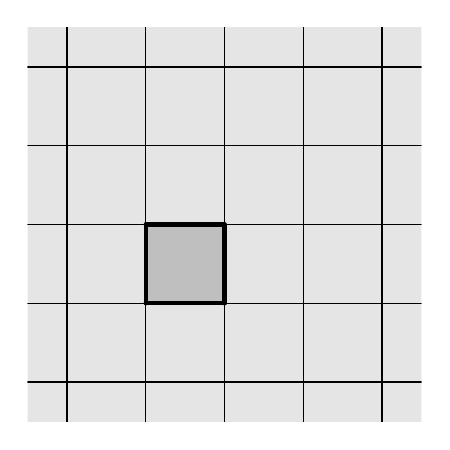
\begin{tikzpicture}[line cap=round,line join=round,>=triangle 45,x=1.0cm,y=1.0cm]
\clip(0.5,0.5) rectangle (5.5,5.5);
\fill[fill=black,fill opacity=0.1] (0,0) -- (1,0) -- (1,1) -- (0,1) -- cycle;
\fill[fill=black,fill opacity=0.1] (1,0) -- (2,0) -- (2,1) -- (1,1) -- cycle;
\fill[fill=black,fill opacity=0.1] (2,0) -- (3,0) -- (3,1) -- (2,1) -- cycle;
\fill[fill=black,fill opacity=0.1] (3,0) -- (4,0) -- (4,1) -- (3,1) -- cycle;
\fill[fill=black,fill opacity=0.1] (4,0) -- (5,0) -- (5,1) -- (4,1) -- cycle;
\fill[fill=black,fill opacity=0.1] (5,0) -- (6,0) -- (6,1) -- (5,1) -- cycle;
\fill[fill=black,fill opacity=0.1] (6,0) -- (7,0) -- (7,1) -- (6,1) -- cycle;
\fill[fill=black,fill opacity=0.1] (7,0) -- (8,0) -- (8,1) -- (7,1) -- cycle;
\fill[fill=black,fill opacity=0.1] (0,1) -- (1,1) -- (1,2) -- (0,2) -- cycle;
\fill[fill=black,fill opacity=0.1] (1,1) -- (2,1) -- (2,2) -- (1,2) -- cycle;
\fill[fill=black,fill opacity=0.1] (2,1) -- (3,1) -- (3,2) -- (2,2) -- cycle;
\fill[fill=black,fill opacity=0.1] (3,1) -- (4,1) -- (4,2) -- (3,2) -- cycle;
\fill[fill=black,fill opacity=0.1] (4,1) -- (5,1) -- (5,2) -- (4,2) -- cycle;
\fill[fill=black,fill opacity=0.1] (5,1) -- (6,1) -- (6,2) -- (5,2) -- cycle;
\fill[fill=black,fill opacity=0.1] (6,1) -- (7,1) -- (7,2) -- (6,2) -- cycle;
\fill[fill=black,fill opacity=0.1] (7,1) -- (8,1) -- (8,2) -- (7,2) -- cycle;
\fill[fill=black,fill opacity=0.1] (0,2) -- (1,2) -- (1,3) -- (0,3) -- cycle;
\fill[fill=black,fill opacity=0.1] (1,2) -- (2,2) -- (2,3) -- (1,3) -- cycle;
\fill[line width=1.6pt,fill=black,fill opacity=0.25] (2,2) -- (3,2) -- (3,3) -- (2,3) -- cycle;
\fill[fill=black,fill opacity=0.1] (3,2) -- (4,2) -- (4,3) -- (3,3) -- cycle;
\fill[fill=black,fill opacity=0.1] (4,2) -- (5,2) -- (5,3) -- (4,3) -- cycle;
\fill[fill=black,fill opacity=0.1] (5,2) -- (6,2) -- (6,3) -- (5,3) -- cycle;
\fill[fill=black,fill opacity=0.1] (6,2) -- (7,2) -- (7,3) -- (6,3) -- cycle;
\fill[fill=black,fill opacity=0.1] (7,2) -- (8,2) -- (8,3) -- (7,3) -- cycle;
\fill[fill=black,fill opacity=0.1] (0,3) -- (1,3) -- (1,4) -- (0,4) -- cycle;
\fill[fill=black,fill opacity=0.1] (1,3) -- (2,3) -- (2,4) -- (1,4) -- cycle;
\fill[fill=black,fill opacity=0.1] (2,3) -- (3,3) -- (3,4) -- (2,4) -- cycle;
\fill[fill=black,fill opacity=0.1] (3,3) -- (4,3) -- (4,4) -- (3,4) -- cycle;
\fill[fill=black,fill opacity=0.1] (4,3) -- (5,3) -- (5,4) -- (4,4) -- cycle;
\fill[fill=black,fill opacity=0.1] (5,3) -- (6,3) -- (6,4) -- (5,4) -- cycle;
\fill[fill=black,fill opacity=0.1] (6,3) -- (7,3) -- (7,4) -- (6,4) -- cycle;
\fill[fill=black,fill opacity=0.1] (7,3) -- (8,3) -- (8,4) -- (7,4) -- cycle;
\fill[fill=black,fill opacity=0.1] (0,4) -- (1,4) -- (1,5) -- (0,5) -- cycle;
\fill[fill=black,fill opacity=0.1] (1,4) -- (2,4) -- (2,5) -- (1,5) -- cycle;
\fill[fill=black,fill opacity=0.1] (2,4) -- (3,4) -- (3,5) -- (2,5) -- cycle;
\fill[fill=black,fill opacity=0.1] (3,4) -- (4,4) -- (4,5) -- (3,5) -- cycle;
\fill[fill=black,fill opacity=0.1] (4,4) -- (5,4) -- (5,5) -- (4,5) -- cycle;
\fill[fill=black,fill opacity=0.1] (5,4) -- (6,4) -- (6,5) -- (5,5) -- cycle;
\fill[fill=black,fill opacity=0.1] (6,4) -- (7,4) -- (7,5) -- (6,5) -- cycle;
\fill[fill=black,fill opacity=0.1] (7,4) -- (8,4) -- (8,5) -- (7,5) -- cycle;
\fill[fill=black,fill opacity=0.1] (0,5) -- (1,5) -- (1,6) -- (0,6) -- cycle;
\fill[fill=black,fill opacity=0.1] (1,5) -- (2,5) -- (2,6) -- (1,6) -- cycle;
\fill[fill=black,fill opacity=0.1] (2,5) -- (3,5) -- (3,6) -- (2,6) -- cycle;
\fill[fill=black,fill opacity=0.1] (3,5) -- (4,5) -- (4,6) -- (3,6) -- cycle;
\fill[fill=black,fill opacity=0.1] (4,5) -- (5,5) -- (5,6) -- (4,6) -- cycle;
\fill[fill=black,fill opacity=0.1] (5,5) -- (6,5) -- (6,6) -- (5,6) -- cycle;
\fill[fill=black,fill opacity=0.1] (6,5) -- (7,5) -- (7,6) -- (6,6) -- cycle;
\fill[fill=black,fill opacity=0.1] (7,5) -- (8,5) -- (8,6) -- (7,6) -- cycle;
\fill[fill=black,fill opacity=0.1] (0,6) -- (1,6) -- (1,7) -- (0,7) -- cycle;
\fill[fill=black,fill opacity=0.1] (1,6) -- (2,6) -- (2,7) -- (1,7) -- cycle;
\fill[fill=black,fill opacity=0.1] (2,6) -- (3,6) -- (3,7) -- (2,7) -- cycle;
\fill[fill=black,fill opacity=0.1] (3,6) -- (4,6) -- (4,7) -- (3,7) -- cycle;
\fill[fill=black,fill opacity=0.1] (4,6) -- (5,6) -- (5,7) -- (4,7) -- cycle;
\fill[fill=black,fill opacity=0.1] (5,6) -- (6,6) -- (6,7) -- (5,7) -- cycle;
\fill[fill=black,fill opacity=0.1] (6,6) -- (7,6) -- (7,7) -- (6,7) -- cycle;
\fill[fill=black,fill opacity=0.1] (7,6) -- (8,6) -- (8,7) -- (7,7) -- cycle;
\fill[fill=black,fill opacity=0.1] (0,7) -- (1,7) -- (1,8) -- (0,8) -- cycle;
\fill[fill=black,fill opacity=0.1] (1,7) -- (2,7) -- (2,8) -- (1,8) -- cycle;
\fill[fill=black,fill opacity=0.1] (2,7) -- (3,7) -- (3,8) -- (2,8) -- cycle;
\fill[fill=black,fill opacity=0.1] (3,7) -- (4,7) -- (4,8) -- (3,8) -- cycle;
\fill[fill=black,fill opacity=0.1] (4,7) -- (5,7) -- (5,8) -- (4,8) -- cycle;
\fill[fill=black,fill opacity=0.1] (5,7) -- (6,7) -- (6,8) -- (5,8) -- cycle;
\fill[fill=black,fill opacity=0.1] (6,7) -- (7,7) -- (7,8) -- (6,8) -- cycle;
\fill[fill=black,fill opacity=0.1] (7,7) -- (8,7) -- (8,8) -- (7,8) -- cycle;
\draw (0,0)-- (1,0);
\draw (1,0)-- (1,1);
\draw (1,1)-- (0,1);
\draw (0,1)-- (0,0);
\draw (1,0)-- (2,0);
\draw (2,0)-- (2,1);
\draw (2,1)-- (1,1);
\draw (1,1)-- (1,0);
\draw (2,0)-- (3,0);
\draw (3,0)-- (3,1);
\draw (3,1)-- (2,1);
\draw (2,1)-- (2,0);
\draw (3,0)-- (4,0);
\draw (4,0)-- (4,1);
\draw (4,1)-- (3,1);
\draw (3,1)-- (3,0);
\draw (4,0)-- (5,0);
\draw (5,0)-- (5,1);
\draw (5,1)-- (4,1);
\draw (4,1)-- (4,0);
\draw (5,0)-- (6,0);
\draw (6,0)-- (6,1);
\draw (6,1)-- (5,1);
\draw (5,1)-- (5,0);
\draw (6,0)-- (7,0);
\draw (7,0)-- (7,1);
\draw (7,1)-- (6,1);
\draw (6,1)-- (6,0);
\draw (7,0)-- (8,0);
\draw (8,0)-- (8,1);
\draw (8,1)-- (7,1);
\draw (7,1)-- (7,0);
\draw (0,1)-- (1,1);
\draw (1,1)-- (1,2);
\draw (1,2)-- (0,2);
\draw (0,2)-- (0,1);
\draw (1,1)-- (2,1);
\draw (2,1)-- (2,2);
\draw (2,2)-- (1,2);
\draw (1,2)-- (1,1);
\draw (2,1)-- (3,1);
\draw (3,1)-- (3,2);
\draw (3,2)-- (2,2);
\draw (2,2)-- (2,1);
\draw (3,1)-- (4,1);
\draw (4,1)-- (4,2);
\draw (4,2)-- (3,2);
\draw (3,2)-- (3,1);
\draw (4,1)-- (5,1);
\draw (5,1)-- (5,2);
\draw (5,2)-- (4,2);
\draw (4,2)-- (4,1);
\draw (5,1)-- (6,1);
\draw (6,1)-- (6,2);
\draw (6,2)-- (5,2);
\draw (5,2)-- (5,1);
\draw (6,1)-- (7,1);
\draw (7,1)-- (7,2);
\draw (7,2)-- (6,2);
\draw (6,2)-- (6,1);
\draw (7,1)-- (8,1);
\draw (8,1)-- (8,2);
\draw (8,2)-- (7,2);
\draw (7,2)-- (7,1);
\draw (0,2)-- (1,2);
\draw (1,2)-- (1,3);
\draw (1,3)-- (0,3);
\draw (0,3)-- (0,2);
\draw (1,2)-- (2,2);
\draw (2,2)-- (2,3);
\draw (2,3)-- (1,3);
\draw (1,3)-- (1,2);
\draw [line width=1.6pt] (2,2)-- (3,2);
\draw [line width=1.6pt] (3,2)-- (3,3);
\draw [line width=1.6pt] (3,3)-- (2,3);
\draw [line width=1.6pt] (2,3)-- (2,2);
\draw (3,2)-- (4,2);
\draw (4,2)-- (4,3);
\draw (4,3)-- (3,3);
\draw (3,3)-- (3,2);
\draw (4,2)-- (5,2);
\draw (5,2)-- (5,3);
\draw (5,3)-- (4,3);
\draw (4,3)-- (4,2);
\draw (5,2)-- (6,2);
\draw (6,2)-- (6,3);
\draw (6,3)-- (5,3);
\draw (5,3)-- (5,2);
\draw (6,2)-- (7,2);
\draw (7,2)-- (7,3);
\draw (7,3)-- (6,3);
\draw (6,3)-- (6,2);
\draw (7,2)-- (8,2);
\draw (8,2)-- (8,3);
\draw (8,3)-- (7,3);
\draw (7,3)-- (7,2);
\draw (0,3)-- (1,3);
\draw (1,3)-- (1,4);
\draw (1,4)-- (0,4);
\draw (0,4)-- (0,3);
\draw (1,3)-- (2,3);
\draw (2,3)-- (2,4);
\draw (2,4)-- (1,4);
\draw (1,4)-- (1,3);
\draw (2,3)-- (3,3);
\draw (3,3)-- (3,4);
\draw (3,4)-- (2,4);
\draw (2,4)-- (2,3);
\draw (3,3)-- (4,3);
\draw (4,3)-- (4,4);
\draw (4,4)-- (3,4);
\draw (3,4)-- (3,3);
\draw (4,3)-- (5,3);
\draw (5,3)-- (5,4);
\draw (5,4)-- (4,4);
\draw (4,4)-- (4,3);
\draw (5,3)-- (6,3);
\draw (6,3)-- (6,4);
\draw (6,4)-- (5,4);
\draw (5,4)-- (5,3);
\draw (6,3)-- (7,3);
\draw (7,3)-- (7,4);
\draw (7,4)-- (6,4);
\draw (6,4)-- (6,3);
\draw (7,3)-- (8,3);
\draw (8,3)-- (8,4);
\draw (8,4)-- (7,4);
\draw (7,4)-- (7,3);
\draw (0,4)-- (1,4);
\draw (1,4)-- (1,5);
\draw (1,5)-- (0,5);
\draw (0,5)-- (0,4);
\draw (1,4)-- (2,4);
\draw (2,4)-- (2,5);
\draw (2,5)-- (1,5);
\draw (1,5)-- (1,4);
\draw (2,4)-- (3,4);
\draw (3,4)-- (3,5);
\draw (3,5)-- (2,5);
\draw (2,5)-- (2,4);
\draw (3,4)-- (4,4);
\draw (4,4)-- (4,5);
\draw (4,5)-- (3,5);
\draw (3,5)-- (3,4);
\draw (4,4)-- (5,4);
\draw (5,4)-- (5,5);
\draw (5,5)-- (4,5);
\draw (4,5)-- (4,4);
\draw (5,4)-- (6,4);
\draw (6,4)-- (6,5);
\draw (6,5)-- (5,5);
\draw (5,5)-- (5,4);
\draw (6,4)-- (7,4);
\draw (7,4)-- (7,5);
\draw (7,5)-- (6,5);
\draw (6,5)-- (6,4);
\draw (7,4)-- (8,4);
\draw (8,4)-- (8,5);
\draw (8,5)-- (7,5);
\draw (7,5)-- (7,4);
\draw (0,5)-- (1,5);
\draw (1,5)-- (1,6);
\draw (1,6)-- (0,6);
\draw (0,6)-- (0,5);
\draw (1,5)-- (2,5);
\draw (2,5)-- (2,6);
\draw (2,6)-- (1,6);
\draw (1,6)-- (1,5);
\draw (2,5)-- (3,5);
\draw (3,5)-- (3,6);
\draw (3,6)-- (2,6);
\draw (2,6)-- (2,5);
\draw (3,5)-- (4,5);
\draw (4,5)-- (4,6);
\draw (4,6)-- (3,6);
\draw (3,6)-- (3,5);
\draw (4,5)-- (5,5);
\draw (5,5)-- (5,6);
\draw (5,6)-- (4,6);
\draw (4,6)-- (4,5);
\draw (5,5)-- (6,5);
\draw (6,5)-- (6,6);
\draw (6,6)-- (5,6);
\draw (5,6)-- (5,5);
\draw (6,5)-- (7,5);
\draw (7,5)-- (7,6);
\draw (7,6)-- (6,6);
\draw (6,6)-- (6,5);
\draw (7,5)-- (8,5);
\draw (8,5)-- (8,6);
\draw (8,6)-- (7,6);
\draw (7,6)-- (7,5);
\draw (0,6)-- (1,6);
\draw (1,6)-- (1,7);
\draw (1,7)-- (0,7);
\draw (0,7)-- (0,6);
\draw (1,6)-- (2,6);
\draw (2,6)-- (2,7);
\draw (2,7)-- (1,7);
\draw (1,7)-- (1,6);
\draw (2,6)-- (3,6);
\draw (3,6)-- (3,7);
\draw (3,7)-- (2,7);
\draw (2,7)-- (2,6);
\draw (3,6)-- (4,6);
\draw (4,6)-- (4,7);
\draw (4,7)-- (3,7);
\draw (3,7)-- (3,6);
\draw (4,6)-- (5,6);
\draw (5,6)-- (5,7);
\draw (5,7)-- (4,7);
\draw (4,7)-- (4,6);
\draw (5,6)-- (6,6);
\draw (6,6)-- (6,7);
\draw (6,7)-- (5,7);
\draw (5,7)-- (5,6);
\draw (6,6)-- (7,6);
\draw (7,6)-- (7,7);
\draw (7,7)-- (6,7);
\draw (6,7)-- (6,6);
\draw (7,6)-- (8,6);
\draw (8,6)-- (8,7);
\draw (8,7)-- (7,7);
\draw (7,7)-- (7,6);
\draw (0,7)-- (1,7);
\draw (1,7)-- (1,8);
\draw (1,8)-- (0,8);
\draw (0,8)-- (0,7);
\draw (1,7)-- (2,7);
\draw (2,7)-- (2,8);
\draw (2,8)-- (1,8);
\draw (1,8)-- (1,7);
\draw (2,7)-- (3,7);
\draw (3,7)-- (3,8);
\draw (3,8)-- (2,8);
\draw (2,8)-- (2,7);
\draw (3,7)-- (4,7);
\draw (4,7)-- (4,8);
\draw (4,8)-- (3,8);
\draw (3,8)-- (3,7);
\draw (4,7)-- (5,7);
\draw (5,7)-- (5,8);
\draw (5,8)-- (4,8);
\draw (4,8)-- (4,7);
\draw (5,7)-- (6,7);
\draw (6,7)-- (6,8);
\draw (6,8)-- (5,8);
\draw (5,8)-- (5,7);
\draw (6,7)-- (7,7);
\draw (7,7)-- (7,8);
\draw (7,8)-- (6,8);
\draw (6,8)-- (6,7);
\draw (7,7)-- (8,7);
\draw (8,7)-- (8,8);
\draw (8,8)-- (7,8);
\draw (7,8)-- (7,7);
\end{tikzpicture}
}
				\only<5>{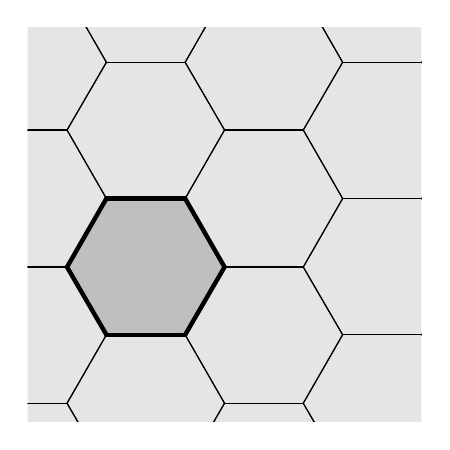
\begin{tikzpicture}[line cap=round,line join=round,>=triangle 45,x=1.0cm,y=1.0cm]
\clip(0.5,1.5) rectangle (5.5,6.5);
\fill[fill=black,fill opacity=0.1] (0,0) -- (1,0) -- (1.5,0.87) -- (1,1.73) -- (0,1.73) -- (-0.5,0.87) -- cycle;
\fill[fill=black,fill opacity=0.1] (1.5,0.87) -- (2.5,0.87) -- (3,1.73) -- (2.5,2.6) -- (1.5,2.6) -- (1,1.73) -- cycle;
\fill[fill=black,fill opacity=0.1] (3,0) -- (4,0) -- (4.5,0.87) -- (4,1.73) -- (3,1.73) -- (2.5,0.87) -- cycle;
\fill[fill=black,fill opacity=0.1] (4.5,0.87) -- (5.5,0.87) -- (6,1.73) -- (5.5,2.6) -- (4.5,2.6) -- (4,1.73) -- cycle;
\fill[fill=black,fill opacity=0.1] (6,0) -- (7,0) -- (7.5,0.87) -- (7,1.73) -- (6,1.73) -- (5.5,0.87) -- cycle;
\fill[fill=black,fill opacity=0.1] (7.5,0.87) -- (8.5,0.87) -- (9,1.73) -- (8.5,2.6) -- (7.5,2.6) -- (7,1.73) -- cycle;
\fill[fill=black,fill opacity=0.1] (9,0) -- (10,0) -- (10.5,0.87) -- (10,1.73) -- (9,1.73) -- (8.5,0.87) -- cycle;
\fill[fill=black,fill opacity=0.1] (10.5,0.87) -- (11.5,0.87) -- (12,1.73) -- (11.5,2.6) -- (10.5,2.6) -- (10,1.73) -- cycle;
\fill[fill=black,fill opacity=0.1] (0,1.73) -- (1,1.73) -- (1.5,2.6) -- (1,3.46) -- (0,3.46) -- (-0.5,2.6) -- cycle;
\fill[line width=1.6pt,fill=black,fill opacity=0.25] (1.5,2.6) -- (2.5,2.6) -- (3,3.46) -- (2.5,4.33) -- (1.5,4.33) -- (1,3.46) -- cycle;
\fill[fill=black,fill opacity=0.1] (3,1.73) -- (4,1.73) -- (4.5,2.6) -- (4,3.46) -- (3,3.46) -- (2.5,2.6) -- cycle;
\fill[fill=black,fill opacity=0.1] (4.5,2.6) -- (5.5,2.6) -- (6,3.46) -- (5.5,4.33) -- (4.5,4.33) -- (4,3.46) -- cycle;
\fill[fill=black,fill opacity=0.1] (6,1.73) -- (7,1.73) -- (7.5,2.6) -- (7,3.46) -- (6,3.46) -- (5.5,2.6) -- cycle;
\fill[fill=black,fill opacity=0.1] (7.5,2.6) -- (8.5,2.6) -- (9,3.46) -- (8.5,4.33) -- (7.5,4.33) -- (7,3.46) -- cycle;
\fill[fill=black,fill opacity=0.1] (9,1.73) -- (10,1.73) -- (10.5,2.6) -- (10,3.46) -- (9,3.46) -- (8.5,2.6) -- cycle;
\fill[fill=black,fill opacity=0.1] (10.5,2.6) -- (11.5,2.6) -- (12,3.46) -- (11.5,4.33) -- (10.5,4.33) -- (10,3.46) -- cycle;
\fill[fill=black,fill opacity=0.1] (0,3.46) -- (1,3.46) -- (1.5,4.33) -- (1,5.2) -- (0,5.2) -- (-0.5,4.33) -- cycle;
\fill[fill=black,fill opacity=0.1] (1.5,4.33) -- (2.5,4.33) -- (3,5.2) -- (2.5,6.06) -- (1.5,6.06) -- (1,5.2) -- cycle;
\fill[fill=black,fill opacity=0.1] (3,3.46) -- (4,3.46) -- (4.5,4.33) -- (4,5.2) -- (3,5.2) -- (2.5,4.33) -- cycle;
\fill[fill=black,fill opacity=0.1] (4.5,4.33) -- (5.5,4.33) -- (6,5.2) -- (5.5,6.06) -- (4.5,6.06) -- (4,5.2) -- cycle;
\fill[fill=black,fill opacity=0.1] (6,3.46) -- (7,3.46) -- (7.5,4.33) -- (7,5.2) -- (6,5.2) -- (5.5,4.33) -- cycle;
\fill[fill=black,fill opacity=0.1] (7.5,4.33) -- (8.5,4.33) -- (9,5.2) -- (8.5,6.06) -- (7.5,6.06) -- (7,5.2) -- cycle;
\fill[fill=black,fill opacity=0.1] (9,3.46) -- (10,3.46) -- (10.5,4.33) -- (10,5.2) -- (9,5.2) -- (8.5,4.33) -- cycle;
\fill[fill=black,fill opacity=0.1] (10.5,4.33) -- (11.5,4.33) -- (12,5.2) -- (11.5,6.06) -- (10.5,6.06) -- (10,5.2) -- cycle;
\fill[fill=black,fill opacity=0.1] (0,5.2) -- (1,5.2) -- (1.5,6.06) -- (1,6.93) -- (0,6.93) -- (-0.5,6.06) -- cycle;
\fill[fill=black,fill opacity=0.1] (1.5,6.06) -- (2.5,6.06) -- (3,6.93) -- (2.5,7.79) -- (1.5,7.79) -- (1,6.93) -- cycle;
\fill[fill=black,fill opacity=0.1] (3,5.2) -- (4,5.2) -- (4.5,6.06) -- (4,6.93) -- (3,6.93) -- (2.5,6.06) -- cycle;
\fill[fill=black,fill opacity=0.1] (4.5,6.06) -- (5.5,6.06) -- (6,6.93) -- (5.5,7.79) -- (4.5,7.79) -- (4,6.93) -- cycle;
\fill[fill=black,fill opacity=0.1] (6,5.2) -- (7,5.2) -- (7.5,6.06) -- (7,6.93) -- (6,6.93) -- (5.5,6.06) -- cycle;
\fill[fill=black,fill opacity=0.1] (7.5,6.06) -- (8.5,6.06) -- (9,6.93) -- (8.5,7.79) -- (7.5,7.79) -- (7,6.93) -- cycle;
\fill[fill=black,fill opacity=0.1] (9,5.2) -- (10,5.2) -- (10.5,6.06) -- (10,6.93) -- (9,6.93) -- (8.5,6.06) -- cycle;
\fill[fill=black,fill opacity=0.1] (10.5,6.06) -- (11.5,6.06) -- (12,6.93) -- (11.5,7.79) -- (10.5,7.79) -- (10,6.93) -- cycle;
\fill[fill=black,fill opacity=0.1] (0,6.93) -- (1,6.93) -- (1.5,7.79) -- (1,8.66) -- (0,8.66) -- (-0.5,7.79) -- cycle;
\fill[fill=black,fill opacity=0.1] (1.5,7.79) -- (2.5,7.79) -- (3,8.66) -- (2.5,9.53) -- (1.5,9.53) -- (1,8.66) -- cycle;
\fill[fill=black,fill opacity=0.1] (3,6.93) -- (4,6.93) -- (4.5,7.79) -- (4,8.66) -- (3,8.66) -- (2.5,7.79) -- cycle;
\fill[fill=black,fill opacity=0.1] (4.5,7.79) -- (5.5,7.79) -- (6,8.66) -- (5.5,9.53) -- (4.5,9.53) -- (4,8.66) -- cycle;
\fill[fill=black,fill opacity=0.1] (6,6.93) -- (7,6.93) -- (7.5,7.79) -- (7,8.66) -- (6,8.66) -- (5.5,7.79) -- cycle;
\fill[fill=black,fill opacity=0.1] (7.5,7.79) -- (8.5,7.79) -- (9,8.66) -- (8.5,9.53) -- (7.5,9.53) -- (7,8.66) -- cycle;
\fill[fill=black,fill opacity=0.1] (9,6.93) -- (10,6.93) -- (10.5,7.79) -- (10,8.66) -- (9,8.66) -- (8.5,7.79) -- cycle;
\fill[fill=black,fill opacity=0.1] (10.5,7.79) -- (11.5,7.79) -- (12,8.66) -- (11.5,9.53) -- (10.5,9.53) -- (10,8.66) -- cycle;
\fill[fill=black,fill opacity=0.1] (0,8.66) -- (1,8.66) -- (1.5,9.53) -- (1,10.39) -- (0,10.39) -- (-0.5,9.53) -- cycle;
\fill[fill=black,fill opacity=0.1] (1.5,9.53) -- (2.5,9.53) -- (3,10.39) -- (2.5,11.26) -- (1.5,11.26) -- (1,10.39) -- cycle;
\fill[fill=black,fill opacity=0.1] (3,8.66) -- (4,8.66) -- (4.5,9.53) -- (4,10.39) -- (3,10.39) -- (2.5,9.53) -- cycle;
\fill[fill=black,fill opacity=0.1] (4.5,9.53) -- (5.5,9.53) -- (6,10.39) -- (5.5,11.26) -- (4.5,11.26) -- (4,10.39) -- cycle;
\fill[fill=black,fill opacity=0.1] (6,8.66) -- (7,8.66) -- (7.5,9.53) -- (7,10.39) -- (6,10.39) -- (5.5,9.53) -- cycle;
\fill[fill=black,fill opacity=0.1] (7.5,9.53) -- (8.5,9.53) -- (9,10.39) -- (8.5,11.26) -- (7.5,11.26) -- (7,10.39) -- cycle;
\fill[fill=black,fill opacity=0.1] (9,8.66) -- (10,8.66) -- (10.5,9.53) -- (10,10.39) -- (9,10.39) -- (8.5,9.53) -- cycle;
\fill[fill=black,fill opacity=0.1] (10.5,9.53) -- (11.5,9.53) -- (12,10.39) -- (11.5,11.26) -- (10.5,11.26) -- (10,10.39) -- cycle;
\fill[fill=black,fill opacity=0.1] (0,10.39) -- (1,10.39) -- (1.5,11.26) -- (1,12.12) -- (0,12.12) -- (-0.5,11.26) -- cycle;
\fill[fill=black,fill opacity=0.1] (1.5,11.26) -- (2.5,11.26) -- (3,12.12) -- (2.5,12.99) -- (1.5,12.99) -- (1,12.12) -- cycle;
\fill[fill=black,fill opacity=0.1] (3,10.39) -- (4,10.39) -- (4.5,11.26) -- (4,12.12) -- (3,12.12) -- (2.5,11.26) -- cycle;
\fill[fill=black,fill opacity=0.1] (4.5,11.26) -- (5.5,11.26) -- (6,12.12) -- (5.5,12.99) -- (4.5,12.99) -- (4,12.12) -- cycle;
\fill[fill=black,fill opacity=0.1] (6,10.39) -- (7,10.39) -- (7.5,11.26) -- (7,12.12) -- (6,12.12) -- (5.5,11.26) -- cycle;
\fill[fill=black,fill opacity=0.1] (7.5,11.26) -- (8.5,11.26) -- (9,12.12) -- (8.5,12.99) -- (7.5,12.99) -- (7,12.12) -- cycle;
\fill[fill=black,fill opacity=0.1] (9,10.39) -- (10,10.39) -- (10.5,11.26) -- (10,12.12) -- (9,12.12) -- (8.5,11.26) -- cycle;
\fill[fill=black,fill opacity=0.1] (10.5,11.26) -- (11.5,11.26) -- (12,12.12) -- (11.5,12.99) -- (10.5,12.99) -- (10,12.12) -- cycle;
\fill[fill=black,fill opacity=0.1] (0,12.12) -- (1,12.12) -- (1.5,12.99) -- (1,13.86) -- (0,13.86) -- (-0.5,12.99) -- cycle;
\fill[fill=black,fill opacity=0.1] (1.5,12.99) -- (2.5,12.99) -- (3,13.86) -- (2.5,14.72) -- (1.5,14.72) -- (1,13.86) -- cycle;
\fill[fill=black,fill opacity=0.1] (3,12.12) -- (4,12.12) -- (4.5,12.99) -- (4,13.86) -- (3,13.86) -- (2.5,12.99) -- cycle;
\fill[fill=black,fill opacity=0.1] (4.5,12.99) -- (5.5,12.99) -- (6,13.86) -- (5.5,14.72) -- (4.5,14.72) -- (4,13.86) -- cycle;
\fill[fill=black,fill opacity=0.1] (6,12.12) -- (7,12.12) -- (7.5,12.99) -- (7,13.86) -- (6,13.86) -- (5.5,12.99) -- cycle;
\fill[fill=black,fill opacity=0.1] (7.5,12.99) -- (8.5,12.99) -- (9,13.86) -- (8.5,14.72) -- (7.5,14.72) -- (7,13.86) -- cycle;
\fill[fill=black,fill opacity=0.1] (9,12.12) -- (10,12.12) -- (10.5,12.99) -- (10,13.86) -- (9,13.86) -- (8.5,12.99) -- cycle;
\fill[fill=black,fill opacity=0.1] (10.5,12.99) -- (11.5,12.99) -- (12,13.86) -- (11.5,14.72) -- (10.5,14.72) -- (10,13.86) -- cycle;
\draw (0,0)-- (1,0);
\draw (1,0)-- (1.5,0.87);
\draw (1.5,0.87)-- (1,1.73);
\draw (1,1.73)-- (0,1.73);
\draw (0,1.73)-- (-0.5,0.87);
\draw (-0.5,0.87)-- (0,0);
\draw (1.5,0.87)-- (2.5,0.87);
\draw (2.5,0.87)-- (3,1.73);
\draw (3,1.73)-- (2.5,2.6);
\draw (2.5,2.6)-- (1.5,2.6);
\draw (1.5,2.6)-- (1,1.73);
\draw (1,1.73)-- (1.5,0.87);
\draw (3,0)-- (4,0);
\draw (4,0)-- (4.5,0.87);
\draw (4.5,0.87)-- (4,1.73);
\draw (4,1.73)-- (3,1.73);
\draw (3,1.73)-- (2.5,0.87);
\draw (2.5,0.87)-- (3,0);
\draw (4.5,0.87)-- (5.5,0.87);
\draw (5.5,0.87)-- (6,1.73);
\draw (6,1.73)-- (5.5,2.6);
\draw (5.5,2.6)-- (4.5,2.6);
\draw (4.5,2.6)-- (4,1.73);
\draw (4,1.73)-- (4.5,0.87);
\draw (6,0)-- (7,0);
\draw (7,0)-- (7.5,0.87);
\draw (7.5,0.87)-- (7,1.73);
\draw (7,1.73)-- (6,1.73);
\draw (6,1.73)-- (5.5,0.87);
\draw (5.5,0.87)-- (6,0);
\draw (7.5,0.87)-- (8.5,0.87);
\draw (8.5,0.87)-- (9,1.73);
\draw (9,1.73)-- (8.5,2.6);
\draw (8.5,2.6)-- (7.5,2.6);
\draw (7.5,2.6)-- (7,1.73);
\draw (7,1.73)-- (7.5,0.87);
\draw (9,0)-- (10,0);
\draw (10,0)-- (10.5,0.87);
\draw (10.5,0.87)-- (10,1.73);
\draw (10,1.73)-- (9,1.73);
\draw (9,1.73)-- (8.5,0.87);
\draw (8.5,0.87)-- (9,0);
\draw (10.5,0.87)-- (11.5,0.87);
\draw (11.5,0.87)-- (12,1.73);
\draw (12,1.73)-- (11.5,2.6);
\draw (11.5,2.6)-- (10.5,2.6);
\draw (10.5,2.6)-- (10,1.73);
\draw (10,1.73)-- (10.5,0.87);
\draw (0,1.73)-- (1,1.73);
\draw (1,1.73)-- (1.5,2.6);
\draw (1.5,2.6)-- (1,3.46);
\draw (1,3.46)-- (0,3.46);
\draw (0,3.46)-- (-0.5,2.6);
\draw (-0.5,2.6)-- (0,1.73);
\draw [line width=1.6pt] (1.5,2.6)-- (2.5,2.6);
\draw [line width=1.6pt] (2.5,2.6)-- (3,3.46);
\draw [line width=1.6pt] (3,3.46)-- (2.5,4.33);
\draw [line width=1.6pt] (2.5,4.33)-- (1.5,4.33);
\draw [line width=1.6pt] (1.5,4.33)-- (1,3.46);
\draw [line width=1.6pt] (1,3.46)-- (1.5,2.6);
\draw (3,1.73)-- (4,1.73);
\draw (4,1.73)-- (4.5,2.6);
\draw (4.5,2.6)-- (4,3.46);
\draw (4,3.46)-- (3,3.46);
\draw (3,3.46)-- (2.5,2.6);
\draw (2.5,2.6)-- (3,1.73);
\draw (4.5,2.6)-- (5.5,2.6);
\draw (5.5,2.6)-- (6,3.46);
\draw (6,3.46)-- (5.5,4.33);
\draw (5.5,4.33)-- (4.5,4.33);
\draw (4.5,4.33)-- (4,3.46);
\draw (4,3.46)-- (4.5,2.6);
\draw (6,1.73)-- (7,1.73);
\draw (7,1.73)-- (7.5,2.6);
\draw (7.5,2.6)-- (7,3.46);
\draw (7,3.46)-- (6,3.46);
\draw (6,3.46)-- (5.5,2.6);
\draw (5.5,2.6)-- (6,1.73);
\draw (7.5,2.6)-- (8.5,2.6);
\draw (8.5,2.6)-- (9,3.46);
\draw (9,3.46)-- (8.5,4.33);
\draw (8.5,4.33)-- (7.5,4.33);
\draw (7.5,4.33)-- (7,3.46);
\draw (7,3.46)-- (7.5,2.6);
\draw (9,1.73)-- (10,1.73);
\draw (10,1.73)-- (10.5,2.6);
\draw (10.5,2.6)-- (10,3.46);
\draw (10,3.46)-- (9,3.46);
\draw (9,3.46)-- (8.5,2.6);
\draw (8.5,2.6)-- (9,1.73);
\draw (10.5,2.6)-- (11.5,2.6);
\draw (11.5,2.6)-- (12,3.46);
\draw (12,3.46)-- (11.5,4.33);
\draw (11.5,4.33)-- (10.5,4.33);
\draw (10.5,4.33)-- (10,3.46);
\draw (10,3.46)-- (10.5,2.6);
\draw (0,3.46)-- (1,3.46);
\draw (1,3.46)-- (1.5,4.33);
\draw (1.5,4.33)-- (1,5.2);
\draw (1,5.2)-- (0,5.2);
\draw (0,5.2)-- (-0.5,4.33);
\draw (-0.5,4.33)-- (0,3.46);
\draw (1.5,4.33)-- (2.5,4.33);
\draw (2.5,4.33)-- (3,5.2);
\draw (3,5.2)-- (2.5,6.06);
\draw (2.5,6.06)-- (1.5,6.06);
\draw (1.5,6.06)-- (1,5.2);
\draw (1,5.2)-- (1.5,4.33);
\draw (3,3.46)-- (4,3.46);
\draw (4,3.46)-- (4.5,4.33);
\draw (4.5,4.33)-- (4,5.2);
\draw (4,5.2)-- (3,5.2);
\draw (3,5.2)-- (2.5,4.33);
\draw (2.5,4.33)-- (3,3.46);
\draw (4.5,4.33)-- (5.5,4.33);
\draw (5.5,4.33)-- (6,5.2);
\draw (6,5.2)-- (5.5,6.06);
\draw (5.5,6.06)-- (4.5,6.06);
\draw (4.5,6.06)-- (4,5.2);
\draw (4,5.2)-- (4.5,4.33);
\draw (6,3.46)-- (7,3.46);
\draw (7,3.46)-- (7.5,4.33);
\draw (7.5,4.33)-- (7,5.2);
\draw (7,5.2)-- (6,5.2);
\draw (6,5.2)-- (5.5,4.33);
\draw (5.5,4.33)-- (6,3.46);
\draw (7.5,4.33)-- (8.5,4.33);
\draw (8.5,4.33)-- (9,5.2);
\draw (9,5.2)-- (8.5,6.06);
\draw (8.5,6.06)-- (7.5,6.06);
\draw (7.5,6.06)-- (7,5.2);
\draw (7,5.2)-- (7.5,4.33);
\draw (9,3.46)-- (10,3.46);
\draw (10,3.46)-- (10.5,4.33);
\draw (10.5,4.33)-- (10,5.2);
\draw (10,5.2)-- (9,5.2);
\draw (9,5.2)-- (8.5,4.33);
\draw (8.5,4.33)-- (9,3.46);
\draw (10.5,4.33)-- (11.5,4.33);
\draw (11.5,4.33)-- (12,5.2);
\draw (12,5.2)-- (11.5,6.06);
\draw (11.5,6.06)-- (10.5,6.06);
\draw (10.5,6.06)-- (10,5.2);
\draw (10,5.2)-- (10.5,4.33);
\draw (0,5.2)-- (1,5.2);
\draw (1,5.2)-- (1.5,6.06);
\draw (1.5,6.06)-- (1,6.93);
\draw (1,6.93)-- (0,6.93);
\draw (0,6.93)-- (-0.5,6.06);
\draw (-0.5,6.06)-- (0,5.2);
\draw (1.5,6.06)-- (2.5,6.06);
\draw (2.5,6.06)-- (3,6.93);
\draw (3,6.93)-- (2.5,7.79);
\draw (2.5,7.79)-- (1.5,7.79);
\draw (1.5,7.79)-- (1,6.93);
\draw (1,6.93)-- (1.5,6.06);
\draw (3,5.2)-- (4,5.2);
\draw (4,5.2)-- (4.5,6.06);
\draw (4.5,6.06)-- (4,6.93);
\draw (4,6.93)-- (3,6.93);
\draw (3,6.93)-- (2.5,6.06);
\draw (2.5,6.06)-- (3,5.2);
\draw (4.5,6.06)-- (5.5,6.06);
\draw (5.5,6.06)-- (6,6.93);
\draw (6,6.93)-- (5.5,7.79);
\draw (5.5,7.79)-- (4.5,7.79);
\draw (4.5,7.79)-- (4,6.93);
\draw (4,6.93)-- (4.5,6.06);
\draw (6,5.2)-- (7,5.2);
\draw (7,5.2)-- (7.5,6.06);
\draw (7.5,6.06)-- (7,6.93);
\draw (7,6.93)-- (6,6.93);
\draw (6,6.93)-- (5.5,6.06);
\draw (5.5,6.06)-- (6,5.2);
\draw (7.5,6.06)-- (8.5,6.06);
\draw (8.5,6.06)-- (9,6.93);
\draw (9,6.93)-- (8.5,7.79);
\draw (8.5,7.79)-- (7.5,7.79);
\draw (7.5,7.79)-- (7,6.93);
\draw (7,6.93)-- (7.5,6.06);
\draw (9,5.2)-- (10,5.2);
\draw (10,5.2)-- (10.5,6.06);
\draw (10.5,6.06)-- (10,6.93);
\draw (10,6.93)-- (9,6.93);
\draw (9,6.93)-- (8.5,6.06);
\draw (8.5,6.06)-- (9,5.2);
\draw (10.5,6.06)-- (11.5,6.06);
\draw (11.5,6.06)-- (12,6.93);
\draw (12,6.93)-- (11.5,7.79);
\draw (11.5,7.79)-- (10.5,7.79);
\draw (10.5,7.79)-- (10,6.93);
\draw (10,6.93)-- (10.5,6.06);
\draw (0,6.93)-- (1,6.93);
\draw (1,6.93)-- (1.5,7.79);
\draw (1.5,7.79)-- (1,8.66);
\draw (1,8.66)-- (0,8.66);
\draw (0,8.66)-- (-0.5,7.79);
\draw (-0.5,7.79)-- (0,6.93);
\draw (1.5,7.79)-- (2.5,7.79);
\draw (2.5,7.79)-- (3,8.66);
\draw (3,8.66)-- (2.5,9.53);
\draw (2.5,9.53)-- (1.5,9.53);
\draw (1.5,9.53)-- (1,8.66);
\draw (1,8.66)-- (1.5,7.79);
\draw (3,6.93)-- (4,6.93);
\draw (4,6.93)-- (4.5,7.79);
\draw (4.5,7.79)-- (4,8.66);
\draw (4,8.66)-- (3,8.66);
\draw (3,8.66)-- (2.5,7.79);
\draw (2.5,7.79)-- (3,6.93);
\draw (4.5,7.79)-- (5.5,7.79);
\draw (5.5,7.79)-- (6,8.66);
\draw (6,8.66)-- (5.5,9.53);
\draw (5.5,9.53)-- (4.5,9.53);
\draw (4.5,9.53)-- (4,8.66);
\draw (4,8.66)-- (4.5,7.79);
\draw (6,6.93)-- (7,6.93);
\draw (7,6.93)-- (7.5,7.79);
\draw (7.5,7.79)-- (7,8.66);
\draw (7,8.66)-- (6,8.66);
\draw (6,8.66)-- (5.5,7.79);
\draw (5.5,7.79)-- (6,6.93);
\draw (7.5,7.79)-- (8.5,7.79);
\draw (8.5,7.79)-- (9,8.66);
\draw (9,8.66)-- (8.5,9.53);
\draw (8.5,9.53)-- (7.5,9.53);
\draw (7.5,9.53)-- (7,8.66);
\draw (7,8.66)-- (7.5,7.79);
\draw (9,6.93)-- (10,6.93);
\draw (10,6.93)-- (10.5,7.79);
\draw (10.5,7.79)-- (10,8.66);
\draw (10,8.66)-- (9,8.66);
\draw (9,8.66)-- (8.5,7.79);
\draw (8.5,7.79)-- (9,6.93);
\draw (10.5,7.79)-- (11.5,7.79);
\draw (11.5,7.79)-- (12,8.66);
\draw (12,8.66)-- (11.5,9.53);
\draw (11.5,9.53)-- (10.5,9.53);
\draw (10.5,9.53)-- (10,8.66);
\draw (10,8.66)-- (10.5,7.79);
\draw (0,8.66)-- (1,8.66);
\draw (1,8.66)-- (1.5,9.53);
\draw (1.5,9.53)-- (1,10.39);
\draw (1,10.39)-- (0,10.39);
\draw (0,10.39)-- (-0.5,9.53);
\draw (-0.5,9.53)-- (0,8.66);
\draw (1.5,9.53)-- (2.5,9.53);
\draw (2.5,9.53)-- (3,10.39);
\draw (3,10.39)-- (2.5,11.26);
\draw (2.5,11.26)-- (1.5,11.26);
\draw (1.5,11.26)-- (1,10.39);
\draw (1,10.39)-- (1.5,9.53);
\draw (3,8.66)-- (4,8.66);
\draw (4,8.66)-- (4.5,9.53);
\draw (4.5,9.53)-- (4,10.39);
\draw (4,10.39)-- (3,10.39);
\draw (3,10.39)-- (2.5,9.53);
\draw (2.5,9.53)-- (3,8.66);
\draw (4.5,9.53)-- (5.5,9.53);
\draw (5.5,9.53)-- (6,10.39);
\draw (6,10.39)-- (5.5,11.26);
\draw (5.5,11.26)-- (4.5,11.26);
\draw (4.5,11.26)-- (4,10.39);
\draw (4,10.39)-- (4.5,9.53);
\draw (6,8.66)-- (7,8.66);
\draw (7,8.66)-- (7.5,9.53);
\draw (7.5,9.53)-- (7,10.39);
\draw (7,10.39)-- (6,10.39);
\draw (6,10.39)-- (5.5,9.53);
\draw (5.5,9.53)-- (6,8.66);
\draw (7.5,9.53)-- (8.5,9.53);
\draw (8.5,9.53)-- (9,10.39);
\draw (9,10.39)-- (8.5,11.26);
\draw (8.5,11.26)-- (7.5,11.26);
\draw (7.5,11.26)-- (7,10.39);
\draw (7,10.39)-- (7.5,9.53);
\draw (9,8.66)-- (10,8.66);
\draw (10,8.66)-- (10.5,9.53);
\draw (10.5,9.53)-- (10,10.39);
\draw (10,10.39)-- (9,10.39);
\draw (9,10.39)-- (8.5,9.53);
\draw (8.5,9.53)-- (9,8.66);
\draw (10.5,9.53)-- (11.5,9.53);
\draw (11.5,9.53)-- (12,10.39);
\draw (12,10.39)-- (11.5,11.26);
\draw (11.5,11.26)-- (10.5,11.26);
\draw (10.5,11.26)-- (10,10.39);
\draw (10,10.39)-- (10.5,9.53);
\draw (0,10.39)-- (1,10.39);
\draw (1,10.39)-- (1.5,11.26);
\draw (1.5,11.26)-- (1,12.12);
\draw (1,12.12)-- (0,12.12);
\draw (0,12.12)-- (-0.5,11.26);
\draw (-0.5,11.26)-- (0,10.39);
\draw (1.5,11.26)-- (2.5,11.26);
\draw (2.5,11.26)-- (3,12.12);
\draw (3,12.12)-- (2.5,12.99);
\draw (2.5,12.99)-- (1.5,12.99);
\draw (1.5,12.99)-- (1,12.12);
\draw (1,12.12)-- (1.5,11.26);
\draw (3,10.39)-- (4,10.39);
\draw (4,10.39)-- (4.5,11.26);
\draw (4.5,11.26)-- (4,12.12);
\draw (4,12.12)-- (3,12.12);
\draw (3,12.12)-- (2.5,11.26);
\draw (2.5,11.26)-- (3,10.39);
\draw (4.5,11.26)-- (5.5,11.26);
\draw (5.5,11.26)-- (6,12.12);
\draw (6,12.12)-- (5.5,12.99);
\draw (5.5,12.99)-- (4.5,12.99);
\draw (4.5,12.99)-- (4,12.12);
\draw (4,12.12)-- (4.5,11.26);
\draw (6,10.39)-- (7,10.39);
\draw (7,10.39)-- (7.5,11.26);
\draw (7.5,11.26)-- (7,12.12);
\draw (7,12.12)-- (6,12.12);
\draw (6,12.12)-- (5.5,11.26);
\draw (5.5,11.26)-- (6,10.39);
\draw (7.5,11.26)-- (8.5,11.26);
\draw (8.5,11.26)-- (9,12.12);
\draw (9,12.12)-- (8.5,12.99);
\draw (8.5,12.99)-- (7.5,12.99);
\draw (7.5,12.99)-- (7,12.12);
\draw (7,12.12)-- (7.5,11.26);
\draw (9,10.39)-- (10,10.39);
\draw (10,10.39)-- (10.5,11.26);
\draw (10.5,11.26)-- (10,12.12);
\draw (10,12.12)-- (9,12.12);
\draw (9,12.12)-- (8.5,11.26);
\draw (8.5,11.26)-- (9,10.39);
\draw (10.5,11.26)-- (11.5,11.26);
\draw (11.5,11.26)-- (12,12.12);
\draw (12,12.12)-- (11.5,12.99);
\draw (11.5,12.99)-- (10.5,12.99);
\draw (10.5,12.99)-- (10,12.12);
\draw (10,12.12)-- (10.5,11.26);
\draw (0,12.12)-- (1,12.12);
\draw (1,12.12)-- (1.5,12.99);
\draw (1.5,12.99)-- (1,13.86);
\draw (1,13.86)-- (0,13.86);
\draw (0,13.86)-- (-0.5,12.99);
\draw (-0.5,12.99)-- (0,12.12);
\draw (1.5,12.99)-- (2.5,12.99);
\draw (2.5,12.99)-- (3,13.86);
\draw (3,13.86)-- (2.5,14.72);
\draw (2.5,14.72)-- (1.5,14.72);
\draw (1.5,14.72)-- (1,13.86);
\draw (1,13.86)-- (1.5,12.99);
\draw (3,12.12)-- (4,12.12);
\draw (4,12.12)-- (4.5,12.99);
\draw (4.5,12.99)-- (4,13.86);
\draw (4,13.86)-- (3,13.86);
\draw (3,13.86)-- (2.5,12.99);
\draw (2.5,12.99)-- (3,12.12);
\draw (4.5,12.99)-- (5.5,12.99);
\draw (5.5,12.99)-- (6,13.86);
\draw (6,13.86)-- (5.5,14.72);
\draw (5.5,14.72)-- (4.5,14.72);
\draw (4.5,14.72)-- (4,13.86);
\draw (4,13.86)-- (4.5,12.99);
\draw (6,12.12)-- (7,12.12);
\draw (7,12.12)-- (7.5,12.99);
\draw (7.5,12.99)-- (7,13.86);
\draw (7,13.86)-- (6,13.86);
\draw (6,13.86)-- (5.5,12.99);
\draw (5.5,12.99)-- (6,12.12);
\draw (7.5,12.99)-- (8.5,12.99);
\draw (8.5,12.99)-- (9,13.86);
\draw (9,13.86)-- (8.5,14.72);
\draw (8.5,14.72)-- (7.5,14.72);
\draw (7.5,14.72)-- (7,13.86);
\draw (7,13.86)-- (7.5,12.99);
\draw (9,12.12)-- (10,12.12);
\draw (10,12.12)-- (10.5,12.99);
\draw (10.5,12.99)-- (10,13.86);
\draw (10,13.86)-- (9,13.86);
\draw (9,13.86)-- (8.5,12.99);
\draw (8.5,12.99)-- (9,12.12);
\draw (10.5,12.99)-- (11.5,12.99);
\draw (11.5,12.99)-- (12,13.86);
\draw (12,13.86)-- (11.5,14.72);
\draw (11.5,14.72)-- (10.5,14.72);
\draw (10.5,14.72)-- (10,13.86);
\draw (10,13.86)-- (10.5,12.99);
\end{tikzpicture}
}
\end{column}
\begin{column}{0.5\textwidth}
\only<2-5>{\begin{itemize}
\item complete vlakvulling
\item optimale vlakvulling
\item effici\"{e}ntie
\end{itemize}}
    \end{column}
  \end{columns}  
\end{frame}

\begin{frame}
\frametitle{Les 1: Inleiding}
\framesubtitle{Didactische wenken}
\begin{enumerate}
	\item Onderwijsleergesprek / klasgesprek
	\begin{itemize}
	\item Kennismaking met definities
	\end{itemize}
	\item Groepswerk
	\begin{itemize}
	\item Regelmatige veelhoeken in karton uitgeknipt
	\item Experimenteren
	\item Bewijs
	\end{itemize}
  \item Onderwijsleergesprek
  \begin{itemize}
	\item Kennismaking met definities
	\end{itemize}
	\item Groepswerk
	\begin{itemize}
	\item Zelfstandig informatie opzoeken
	\item Raadsels en puzzels oplossen
	\end{itemize}
\end{enumerate}
\end{frame}

\begin{frame}
\begin{columns}
        \begin{column}{0.4\textwidth}
        \begin{figure}[h]
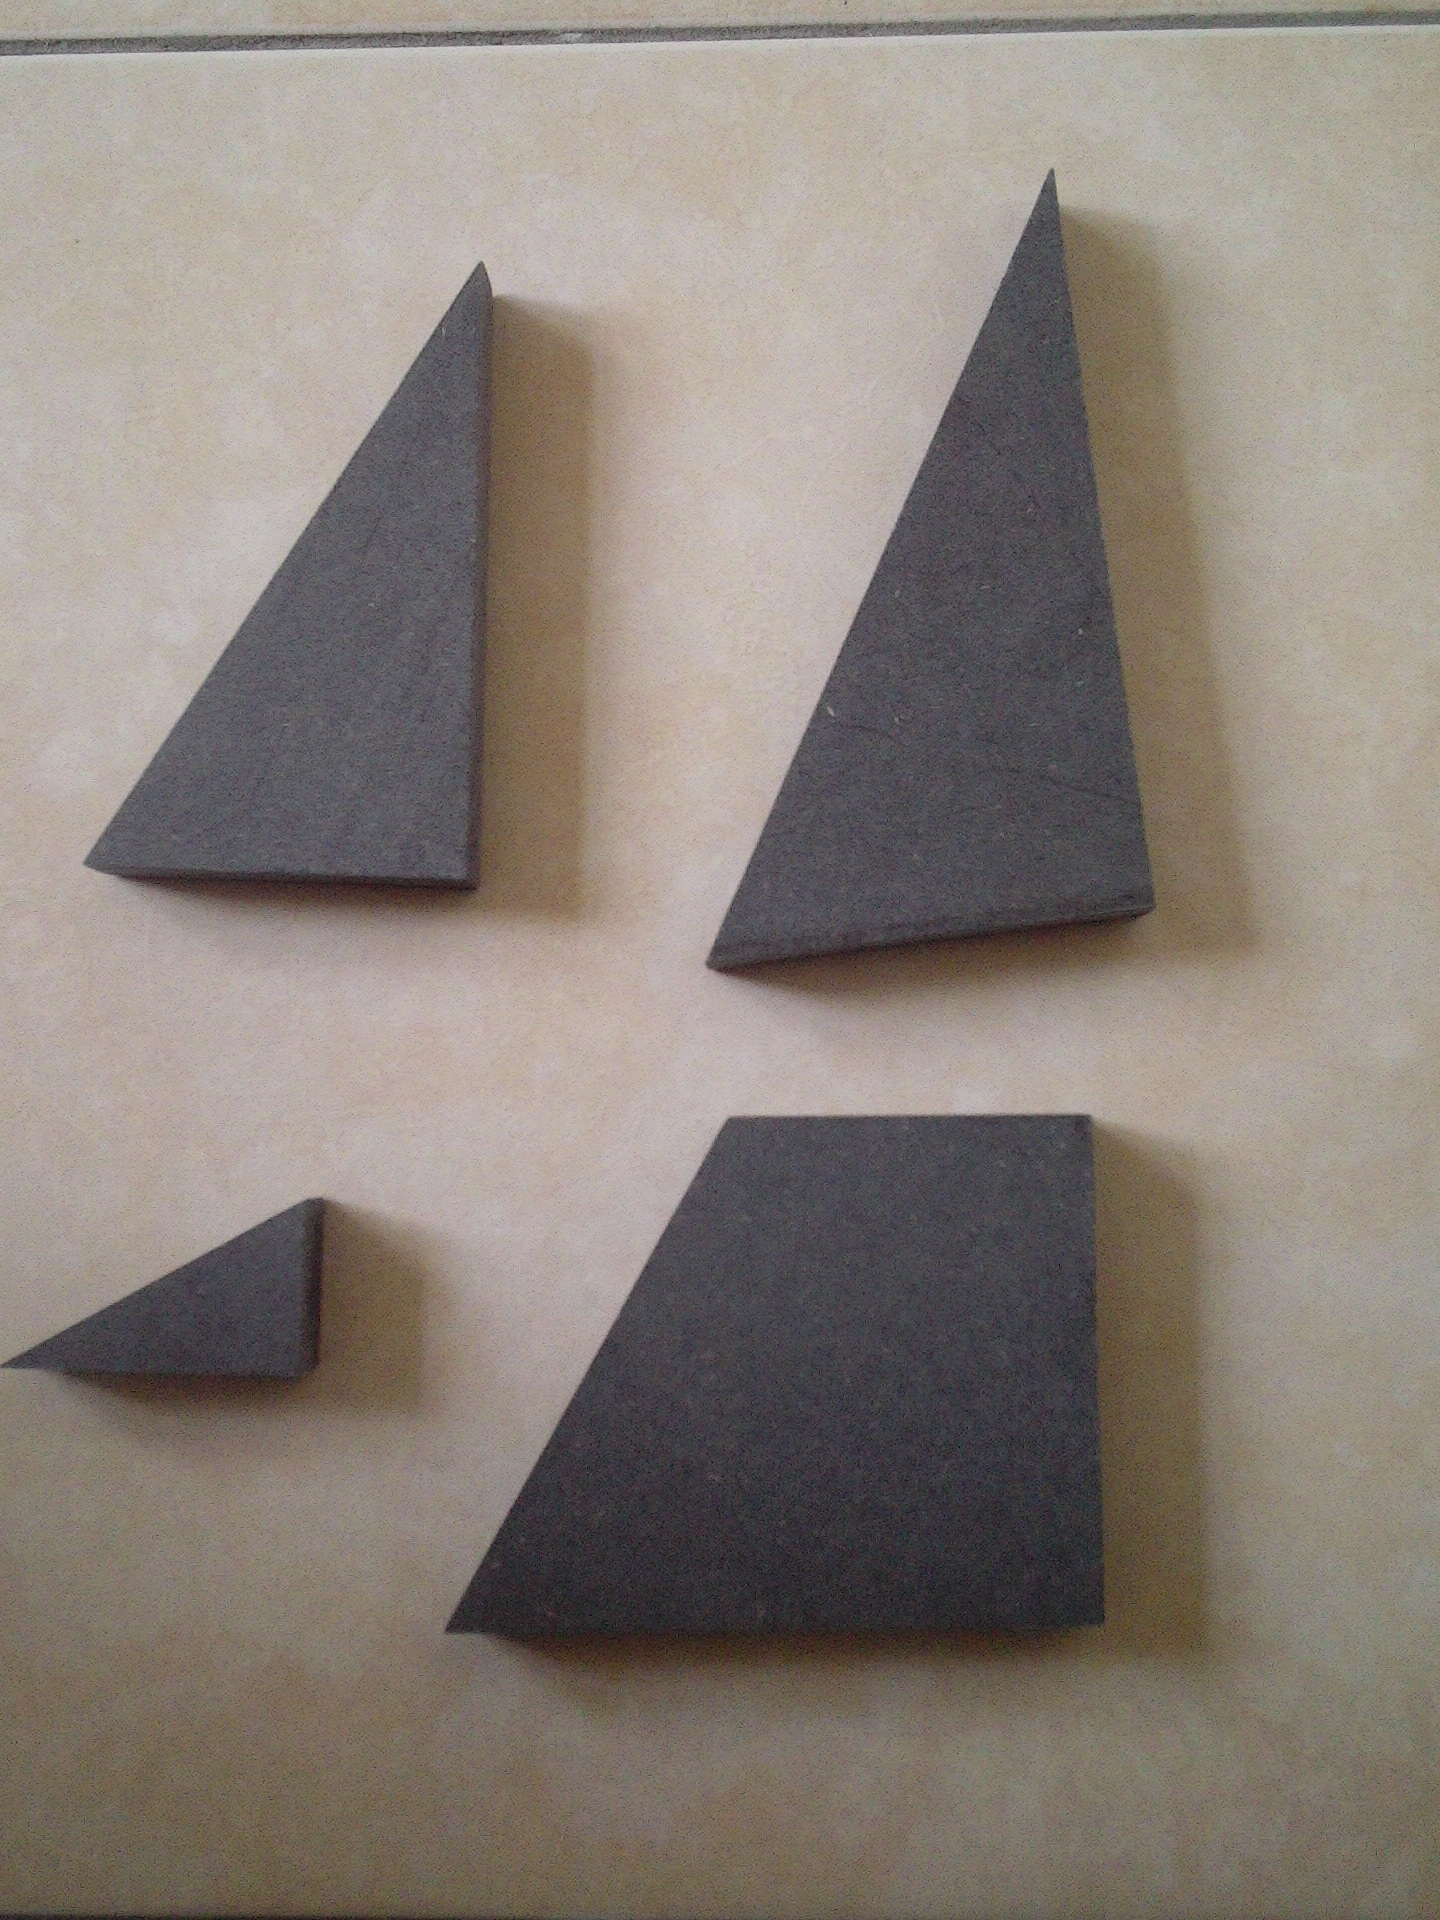
\includegraphics[height=5cm]{PIC0135}%
%\caption{}%
%\label{}%
\end{figure}
\end{column}
\begin{column}{0.4\textwidth}
      
        \begin{figure}[h]
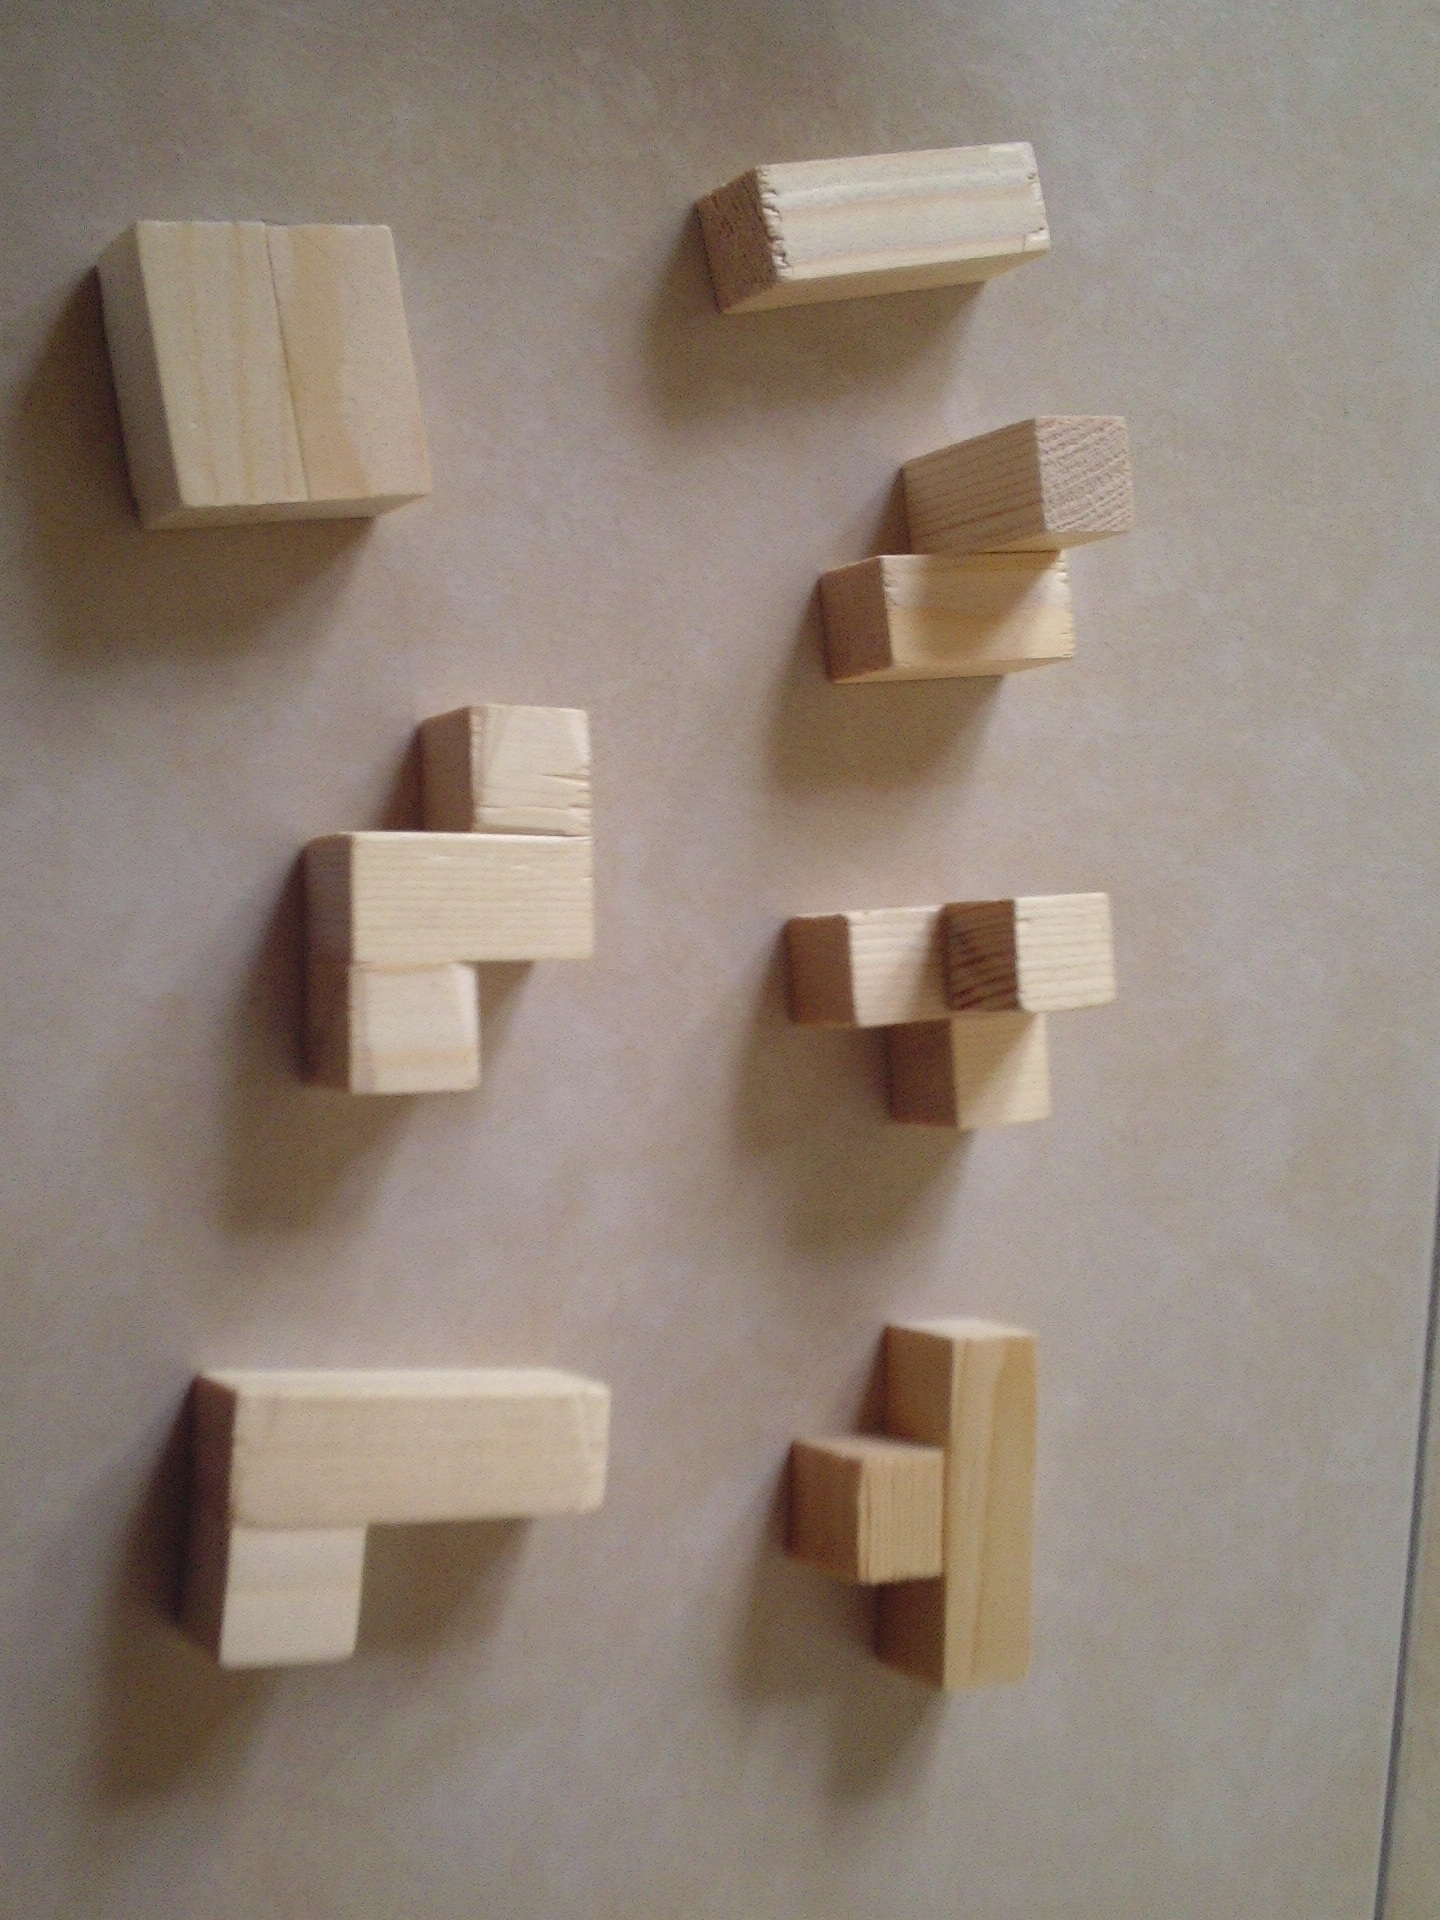
\includegraphics[height=5cm]{PIC0137}%
%\caption{}%
%\label{}%
\end{figure}
    \end{column}
  \end{columns}  
\end{frame}

\begin{frame}
\begin{columns}
        \begin{column}{0.4\textwidth}
        \begin{figure}[h]
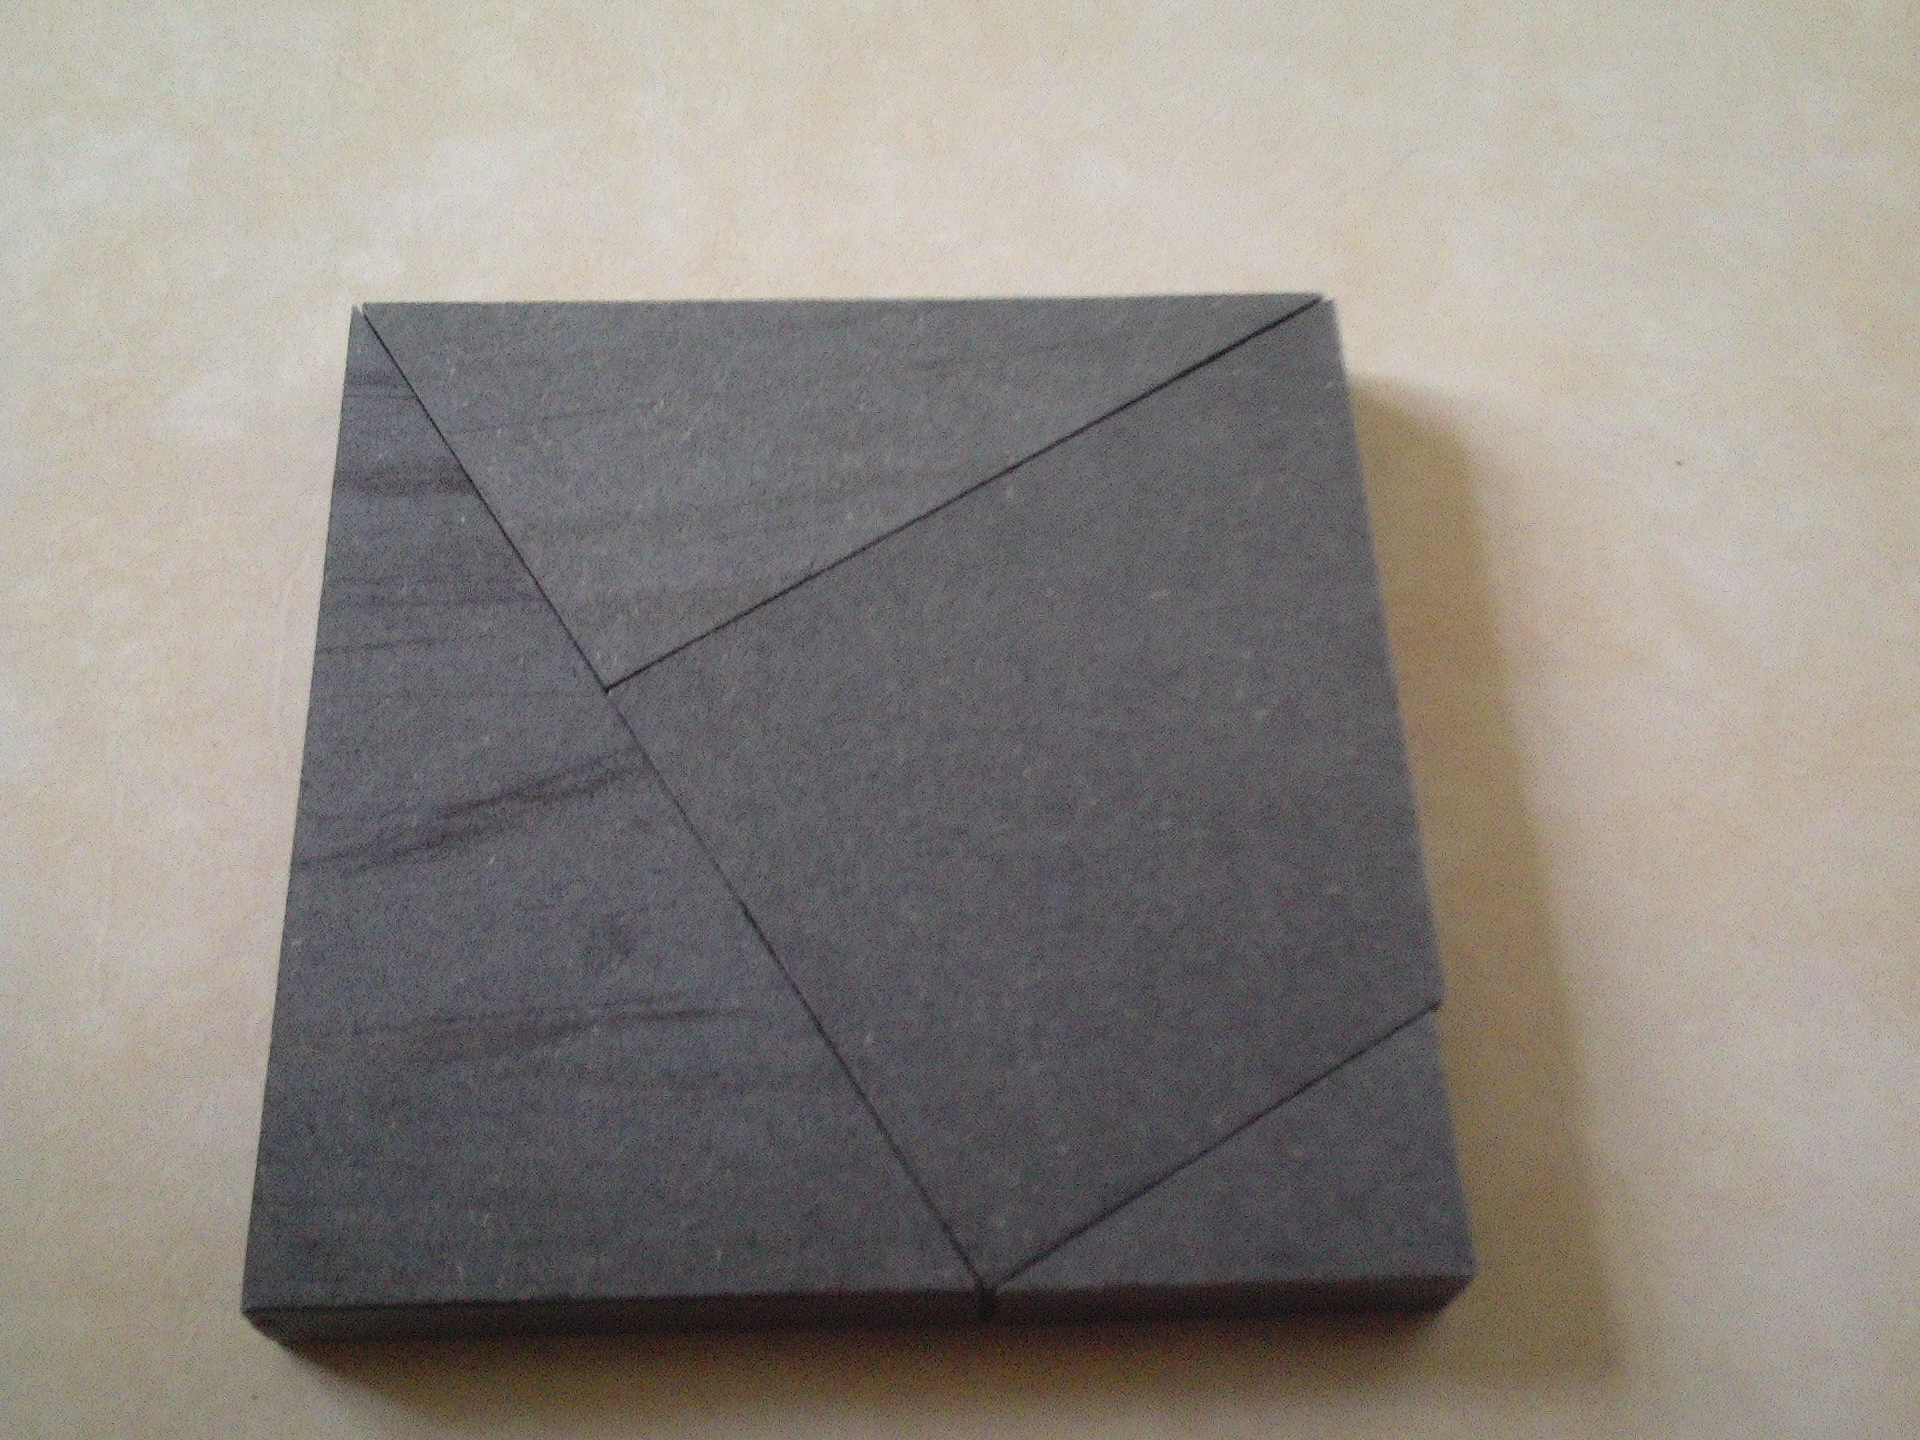
\includegraphics[height=3.5cm]{PIC0134}%
%\caption{}%
%\label{}%
\end{figure}
\end{column}
\begin{column}{0.4\textwidth}
        \begin{figure}[h]
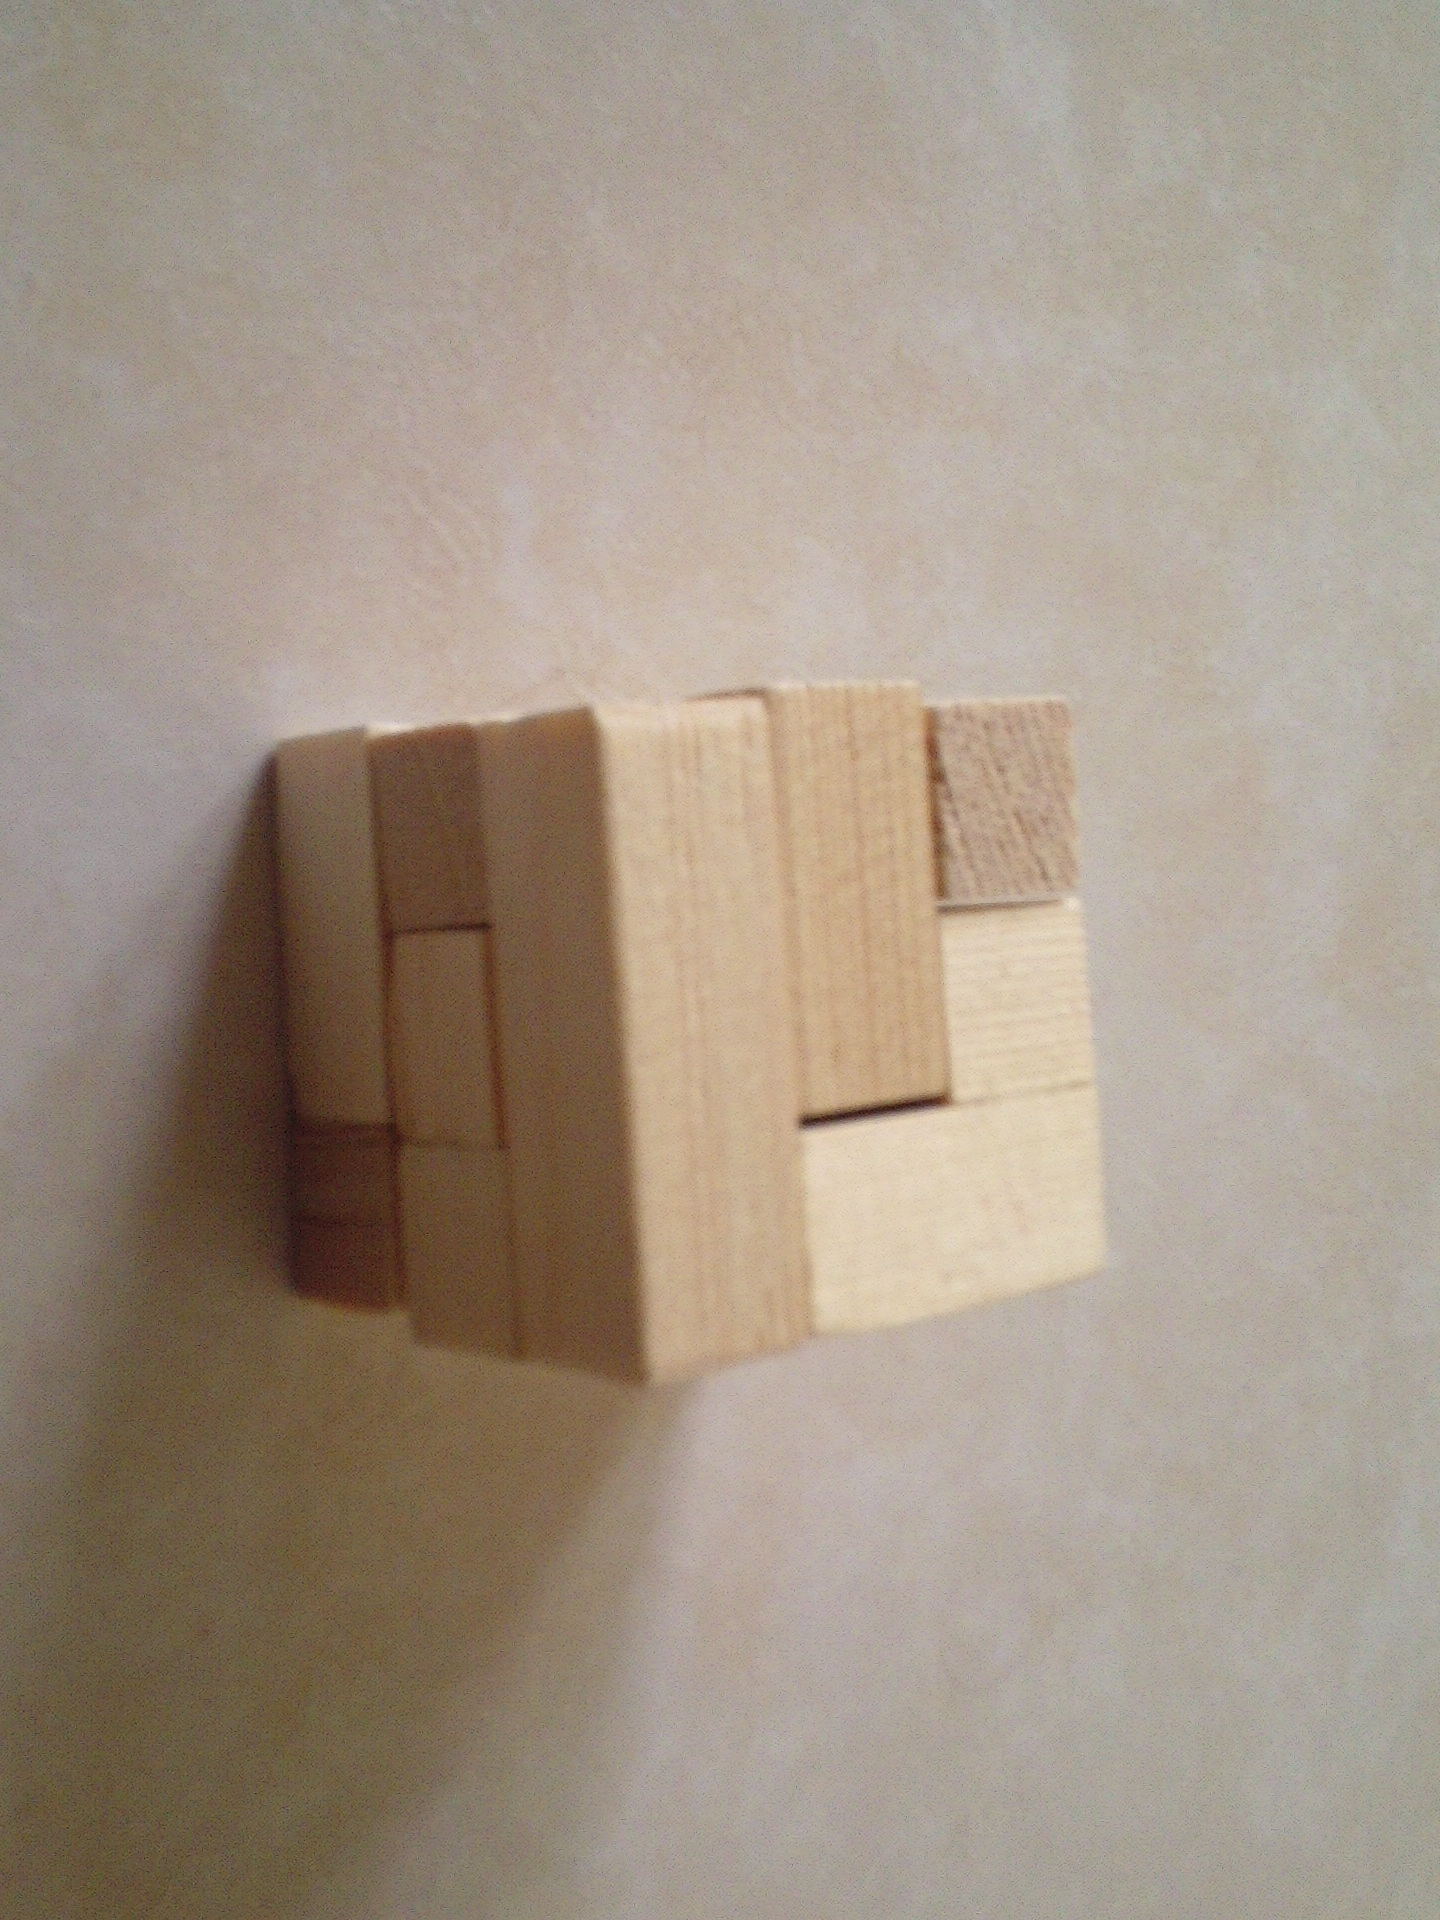
\includegraphics[height=3.5cm]{PIC0136}%
%\caption{}%
%\label{}%
\end{figure}
    \end{column}
  \end{columns}  
\end{frame}

\begin{frame}
\begin{figure}[ht]
\centering
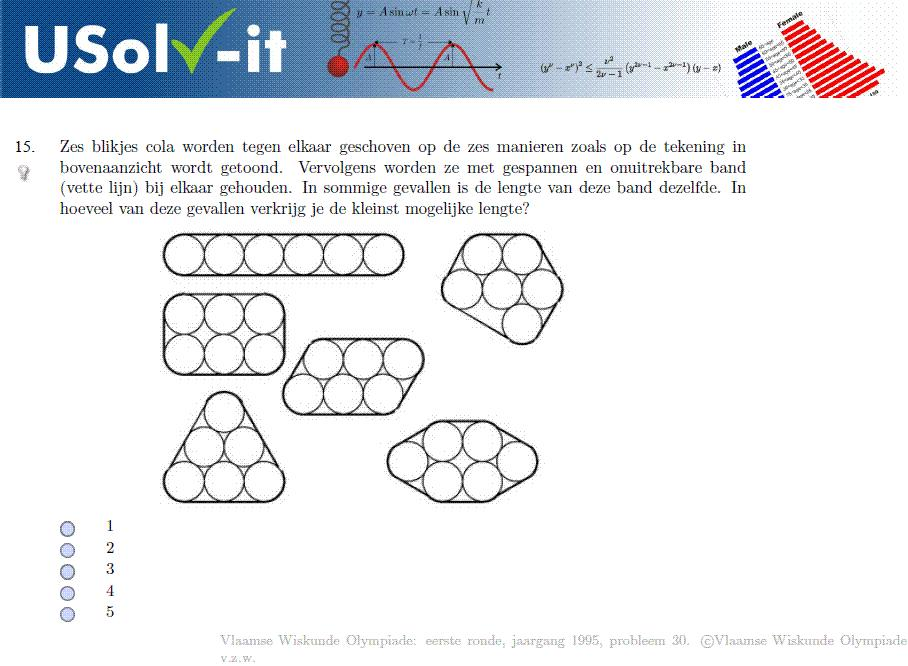
\includegraphics[height=5cm]{vraag}
\label{fig:raadsel}
\caption{Raadsel USolv-IT}
\end{figure}
\end{frame}

\subsection{Les 2: Vullen van vierkanten met kleinere vierkanten en zo tot Perfecte Vierkanten komen}
\begin{frame}
\frametitle{Les 2: Vullen van vierkanten met kleinere vierkanten}
\framesubtitle{Overzicht van de lessen}
\begin{list}{\quad}{}
\item Les 1: Inleiding
\item {\color{blue}Les 2: Vullen van vierkanten met kleinere vierkanten en zo tot Perfecte Vierkanten komen}
\item Les 3: Puzzelen met vierkanten en rechthoeken om vergelijkingen op te lossen
\item Les 4: Kennismaking met tweedimensionale stapelproblemen en het dienbladenprobleem 
\item Les 5: Het dienbladenprobleem: experimenteren en effectief berekenen
\item Les 6: Het dienbladenprobleem: berekenen, bewijzen en besluiten
\item Les 7: Kanonskogels stapelen
\item Les 8: Vervolg kanonskogels en het bolstapelprobleem van Kepler
\end{list}
\end{frame}

\begin{frame}
\frametitle{Les 2: Vullen van vierkanten met kleinere vierkanten}
\framesubtitle{Lesdoelstellingen}
\small
\begin{itemize}
\item De leerlingen kunnen een een vierkant met kleinere vierkanten vullen van de zelfde grootte, om zo een {\bf algemene formule} die de maximale effici\"{e}ntie bepaald, te vinden.
\item De leerlingen weten wat een {\bf perfect vierkant} van orde $n$ is.
\item De leerlingen kunnen een {\bf ondergrens zoeken} voor de orde van het perfect vierkant door redeneren.
\item De leerlingen zien in dat een perfect vierkant dat gedraaid of gespiegeld wordt geen ander perfect vierkant oplevert. Hiervoor leren de leerlingen het begrip {\bf isomorfisme}.
\item De leerlingen beseffen dat het vinden van \'{e}\'{e}n perfect vierkant leidt tot het vinden van een {\bf oneindig aantal} perfecte vierkanten. 
\item De leerlingen kunnen een {\bf bewijs uit het ongerijmde} opstellen om eigenschappen te bewijzen over perfecte vierkanten.
\item De leerlingen kunnen hun resultaten en definities in verband met perfecte vierkanten uitbreiden naar \'{e}\'{e}n en {\bf drie dimensies}.
\end{itemize}
\end{frame}

\begin{frame}
  \frametitle{Les 2: Vullen van vierkanten met kleinere vierkanten}
  \framesubtitle{Didactische wenken}
  \begin{enumerate}
    \item Onderwijsleergesprek 
      \begin{itemize}
        \item Theorie rond perfecte vierkanten ontwikkelen
      \end{itemize}
    \item Individueel werken
      \begin{itemize}
        \item Vullen van een vierkant met kleinere vierkanten van gelijke grootte
        \item Tegenstrijdigheid aantonen als het kleinste vierkantje op de rand wordt gelegd
      \end{itemize}
    \item Leerlingen laten puzzelen
      \begin{itemize}
        \item Bouwplannen voorzien voor de perfecte vierkanten van orde 22
      \end{itemize}
  \end{enumerate}
\end{frame}

\begin{frame}
  \frametitle{Les 2: Vullen van vierkanten met kleinere vierkanten}
  \framesubtitle{Resultaten: vullen van een vierkant met kleinere vierkanten}
  \begin{columns}
    \begin{column}{0.5\textwidth}
      \definecolor{cqcqcq}{rgb}{0.75,0.75,0.75}
\begin{tikzpicture}[scale=0.4,line cap=round,line join=round,>=triangle 45,x=1.0cm,y=1.0cm]
\draw [color=cqcqcq,dash pattern=on 2pt off 2pt, xstep=1.0cm,ystep=1.0cm] (-0.5,-0.5) grid (10.5,10.5);
\clip(-0.5,-0.5) rectangle (10.5,10.5);
\filldraw[line width=1.6pt,fill=black,fill opacity=0.1] (0,0) -- (10,0) -- (10,10) -- (0,10) -- cycle;
\filldraw[fill=black,fill opacity=0.1] (0,0) -- (3,0) -- (3,3) -- (0,3) -- cycle;
\filldraw[fill=black,fill opacity=0.1] (3,0) -- (6,0) -- (6,3) -- (3,3) -- cycle;
\filldraw[fill=black,fill opacity=0.1] (6,0) -- (9,0) -- (9,3) -- (6,3) -- cycle;
\filldraw[fill=black,fill opacity=0.1] (0,3) -- (3,3) -- (3,6) -- (0,6) -- cycle;
\filldraw[fill=black,fill opacity=0.1] (3,3) -- (6,3) -- (6,6) -- (3,6) -- cycle;
\filldraw[fill=black,fill opacity=0.1] (6,3) -- (9,3) -- (9,6) -- (6,6) -- cycle;
\filldraw[fill=black,fill opacity=0.1] (0,6) -- (3,6) -- (3,9) -- (0,9) -- cycle;
\filldraw[fill=black,fill opacity=0.1] (3,6) -- (6,6) -- (6,9) -- (3,9) -- cycle;
\filldraw[fill=black,fill opacity=0.1] (6,6) -- (9,6) -- (9,9) -- (6,9) -- cycle;
\end{tikzpicture}

    \end{column}
    \begin{column}{0.5\textwidth}
    \begin{itemize}
      \item Voorbeeld:
      \begin{align*}
        10^2  &= (3\cdot 3 + 1)^2\\
        \Leftrightarrow 100   &= (3\cdot 3)^2 + 2\cdot 3\cdot 3\cdot 1 + 1^2\\
        \Leftrightarrow 100   &= 81 + 19
      \end{align*}
      \pause
      \item Algemeen:
      \begin{align*}
         a^2  &= (q\cdot d + r)^2\\
        \Leftrightarrow a^2   &= (q\cdot d)^2 + 2\cdot q\cdot d\cdot r + r^2
      \end{align*}
      {\tiny met $a$ de zijde van het grote vierkante, $d$ de zijde van de kleine vierkanten, $q$ het aantal keer we $d$ in $a$ krijgen en $r$ de rest die dan nog overblijft}
    \end{itemize}
    \end{column}
  \end{columns}  
\end{frame}

\begin{frame}
  \frametitle{Les 2: Vullen van vierkanten met kleinere vierkanten}
  \framesubtitle{Alles over perfecte vierkanten}
  \begin{columns}
    \begin{column}{0.4\textwidth}
      \only<1-2>{{\small
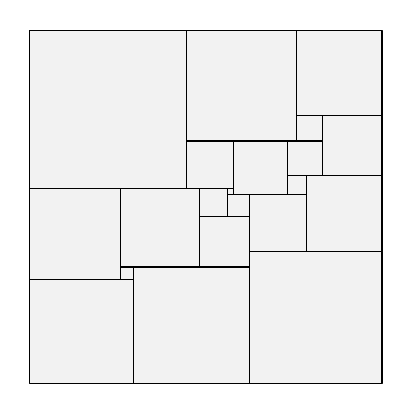
\begin{tikzpicture}[scale=0.04,line cap=round,line join=round,>=triangle 45,x=1.0cm,y=1.0cm]
\clip(-0.5,-0.5) rectangle (113,113);
\filldraw[fill=black,fill opacity=0.05] (0,0) -- (33,0) -- (33,33) -- (0,33) -- cycle;
\filldraw[fill=black,fill opacity=0.05] (33,0) -- (70,0) -- (70,37) -- (33,37) -- cycle;
\filldraw[fill=black,fill opacity=0.05] (70,0) -- (112,0) -- (112,42) -- (70,42) -- cycle;
\filldraw[fill=black,fill opacity=0.05] (0,33) -- (29,33) -- (29,62) -- (0,62) -- cycle;
\filldraw[fill=black,fill opacity=0.05] (29,33) -- (33,33) -- (33,37) -- (29,37) -- cycle;
\filldraw[fill=black,fill opacity=0.05] (0,62) -- (50,62) -- (50,112) -- (0,112) -- cycle;
\filldraw[fill=black,fill opacity=0.05] (29,62) -- (29,37) -- (54,37) -- (54,62) -- cycle;
\filldraw[fill=black,fill opacity=0.05] (54,37) -- (70,37) -- (70,53) -- (54,53) -- cycle;
\filldraw[fill=black,fill opacity=0.05] (70,42) -- (88,42) -- (88,60) -- (70,60) -- cycle;
\filldraw[fill=black,fill opacity=0.05] (88,42) -- (112,42) -- (112,66) -- (88,66) -- cycle;
\filldraw[fill=black,fill opacity=0.05] (54,53) -- (63,53) -- (63,62) -- (54,62) -- cycle;
\filldraw[fill=black,fill opacity=0.05] (63,53) -- (70,53) -- (70,60) -- (63,60) -- cycle;
\filldraw[fill=black,fill opacity=0.05] (63,60) -- (65,60) -- (65,62) -- (63,62) -- cycle;
\filldraw[fill=black,fill opacity=0.05] (82,60) -- (88,60) -- (88,66) -- (82,66) -- cycle;
\filldraw[fill=black,fill opacity=0.05] (65,60) -- (82,60) -- (82,77) -- (65,77) -- cycle;
\filldraw[fill=black,fill opacity=0.05] (50,62) -- (65,62) -- (65,77) -- (50,77) -- cycle;
\filldraw[fill=black,fill opacity=0.05] (50,112) -- (50,77) -- (85,77) -- (85,112) -- cycle;
\filldraw[fill=black,fill opacity=0.05] (82,77) -- (82,66) -- (93,66) -- (93,77) -- cycle;
\filldraw[fill=black,fill opacity=0.05] (93,66) -- (112,66) -- (112,85) -- (93,85) -- cycle;
\filldraw[fill=black,fill opacity=0.05] (85,77) -- (93,77) -- (93,85) -- (85,85) -- cycle;
\filldraw[fill=black,fill opacity=0.05] (85,85) -- (112,85) -- (112,112) -- (85,112) -- cycle;
\end{tikzpicture}
}
}
      \only<3->{{\small
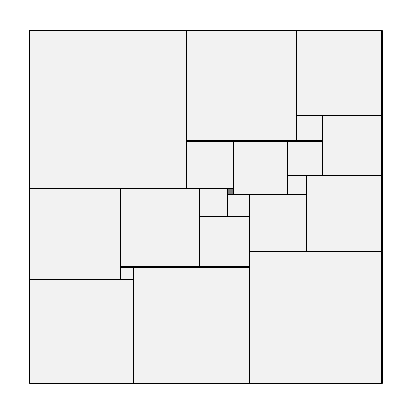
\begin{tikzpicture}[scale=0.04,line cap=round,line join=round,>=triangle 45,x=1.0cm,y=1.0cm]
\clip(-0.5,-0.5) rectangle (113,113);
\filldraw[fill=black,fill opacity=0.05] (0,0) -- (33,0) -- (33,33) -- (0,33) -- cycle;
\filldraw[fill=black,fill opacity=0.05] (33,0) -- (70,0) -- (70,37) -- (33,37) -- cycle;
\filldraw[fill=black,fill opacity=0.05] (70,0) -- (112,0) -- (112,42) -- (70,42) -- cycle;
\filldraw[fill=black,fill opacity=0.05] (0,33) -- (29,33) -- (29,62) -- (0,62) -- cycle;
\filldraw[fill=black,fill opacity=0.05] (29,33) -- (33,33) -- (33,37) -- (29,37) -- cycle;
\filldraw[fill=black,fill opacity=0.05] (0,62) -- (50,62) -- (50,112) -- (0,112) -- cycle;
\filldraw[fill=black,fill opacity=0.05] (29,62) -- (29,37) -- (54,37) -- (54,62) -- cycle;
\filldraw[fill=black,fill opacity=0.05] (54,37) -- (70,37) -- (70,53) -- (54,53) -- cycle;
\filldraw[fill=black,fill opacity=0.05] (70,42) -- (88,42) -- (88,60) -- (70,60) -- cycle;
\filldraw[fill=black,fill opacity=0.05] (88,42) -- (112,42) -- (112,66) -- (88,66) -- cycle;
\filldraw[fill=black,fill opacity=0.05] (54,53) -- (63,53) -- (63,62) -- (54,62) -- cycle;
\filldraw[fill=black,fill opacity=0.05] (63,53) -- (70,53) -- (70,60) -- (63,60) -- cycle;
\filldraw[fill=black,fill opacity=0.5] (63,60) -- (65,60) -- (65,62) -- (63,62) -- cycle;
\filldraw[fill=black,fill opacity=0.05] (82,60) -- (88,60) -- (88,66) -- (82,66) -- cycle;
\filldraw[fill=black,fill opacity=0.05] (65,60) -- (82,60) -- (82,77) -- (65,77) -- cycle;
\filldraw[fill=black,fill opacity=0.05] (50,62) -- (65,62) -- (65,77) -- (50,77) -- cycle;
\filldraw[fill=black,fill opacity=0.05] (50,112) -- (50,77) -- (85,77) -- (85,112) -- cycle;
\filldraw[fill=black,fill opacity=0.05] (82,77) -- (82,66) -- (93,66) -- (93,77) -- cycle;
\filldraw[fill=black,fill opacity=0.05] (93,66) -- (112,66) -- (112,85) -- (93,85) -- cycle;
\filldraw[fill=black,fill opacity=0.05] (85,77) -- (93,77) -- (93,85) -- (85,85) -- cycle;
\filldraw[fill=black,fill opacity=0.05] (85,85) -- (112,85) -- (112,112) -- (85,112) -- cycle;
\end{tikzpicture}
}
}
    \end{column}
    \begin{column}{0.6\textwidth}
    {\scriptsize
      \begin{itemize}
        \item Een {\bf perfect vierkant} is een vierkant dat opgedeeld kan worden in een eindig aantal kleinere vierkanten waarvan geen twee dezelfde grootte hebben.
        \item De {\bf orde} van een perfect vierkant is het aantal kleinere vierkanten dat het bevat.
        \pause
        \item Het vierkant heeft $8$ symmetrie�n, de dihedrale groep $D4$, dus ��n oplossing leidt tot 8 isomorfe oplossingen.
          \begin{center}
            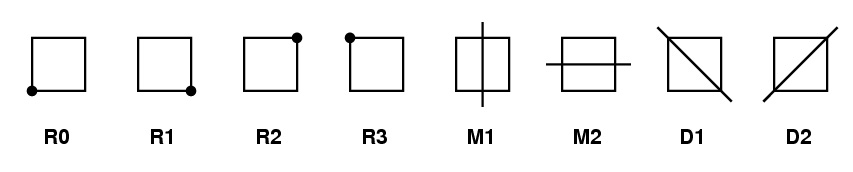
\includegraphics[width=0.8\textwidth]{dih4}
          \end{center}
        \pause
        \item Door het perfecte vierkant te hertekenen binnen het kleinste vierkantje construeren we nieuwe perfecte vierkanten.
        \pause
        \item Een {\bf fractaal} is een meetkundige figuur die zelfgelijkend is. 
      \end{itemize}
    }
    \end{column}
  \end{columns}  
\end{frame}

\begin{frame}
  \frametitle{Les 2: Vullen van vierkanten met kleinere vierkanten}
  \framesubtitle{Eigenschap kleinste vierkantje in een perfect vierkant}
  \begin{columns}
    \begin{column}{0.5\textwidth}
      %\only<1>{\definecolor{cccccc}{rgb}{0.6,0.6,0.6}
\begin{tikzpicture}[scale=0.3, line cap=round,line join=round,>=triangle 45,x=1.0cm,y=1.0cm]
\clip(45,32) rectangle (75,61);
\draw [line width=1.2pt, color=cccccc] (65,32) -- (65,61);
\filldraw[line width=1.2pt,fill=black,fill opacity=0.1] (54,59.12) -- (63,59.12) -- (63,50.12) -- (54,50.12) -- cycle;
\filldraw[line width=1.2pt,fill=black,fill opacity=0.1] (63,59.12) -- (70,59.12) -- (70,52.12) -- (63,52.12) -- cycle;
\filldraw[line width=1.2pt,fill=black,fill opacity=0.15] (63,52.12) -- (65,52.12) -- (65,50.12) -- (63,50.12) -- cycle;
\filldraw[line width=1.2pt,fill=black,fill opacity=0.1] (50,50.12) -- (65,50.12) -- (65,35.12) -- (50,35.12) -- cycle;
\end{tikzpicture}
}
      \definecolor{cccccc}{rgb}{0.6,0.6,0.6}
\begin{tikzpicture}[scale=0.3, line cap=round,line join=round,>=triangle 45,x=1.0cm,y=1.0cm]
\clip(45,32) rectangle (75,61);
\draw [line width=1.2pt, color=cccccc] (65,32) -- (65,61);
\filldraw[line width=1.2pt,fill=black,fill opacity=0.1] (54,59.12) -- (63,59.12) -- (63,50.12) -- (54,50.12) -- cycle;
\filldraw[line width=1.2pt,fill=black,fill opacity=0.1] (63,59.12) -- (70,59.12) -- (70,52.12) -- (63,52.12) -- cycle;
\filldraw[line width=1.2pt,fill=black,fill opacity=0.15] (63,52.12) -- (65,52.12) -- (65,50.12) -- (63,50.12) -- cycle;
\filldraw[line width=1.2pt,fill=black,fill opacity=0.1] (50,50.12) -- (65,50.12) -- (65,35.12) -- (50,35.12) -- cycle;
\end{tikzpicture}

    \end{column}
    \begin{column}{0.5\textwidth}
    {\scriptsize
      \begin{stelling}
      Het kleinste vierkantje in een perfect vierkant kan nooit aan de rand liggen.
      \end{stelling}
      {\tiny
        \begin{list}{}{\leftmargin=0pt}
          \pause
          \item Uit het ongerijmde.
          \item Veronderstel dat het kleinste vierkantje in een perfect vierkant op de rand ligt.
          \pause
          \item Hoeveel vierkantjes liggen dan nog rond het kleinste vierkantje?
          \item Wat weten we over de vierkantjes die rond het kleinste vierkantje liggen?
          \pause
          \item Dus \'e\'en van de vierkantjes komt over de rand!
          \pause
          \item Dus we hebben geen perfect vierkant, een strijdigheid!
          \item Dus het kleinste vierkantje kan niet op de rand liggen!
        \end{list}
      }
    }
    \end{column}
  \end{columns}  
\end{frame}


\subsection{Les 3: Puzzelen met vierkanten en rechthoeken om vergelijkingen op te lossen}
\begin{frame}
\frametitle{Les 3: Vergelijkingen op lossen met oppervlakten}
\framesubtitle{Overzicht van de lessen}
\begin{list}{\quad}{}
\item Les 1: Inleiding
\item Les 2: Vullen van vierkanten met kleinere vierkanten en zo tot Perfecte Vierkanten komen
\item {\color{blue}Les 3: Puzzelen met vierkanten en rechthoeken om vergelijkingen op te lossen}
\item Les 4: Kennismaking met tweedimensionale stapelproblemen en het dienbladenprobleem 
\item Les 5: Het dienbladenprobleem: experimenteren en effectief berekenen
\item Les 6: Het dienbladenprobleem: berekenen, bewijzen en besluiten
\item Les 7: Kanonskogels stapelen
\item Les 8: Vervolg kanonskogels en het bolstapelprobleem van Kepler
\end{list}
\end{frame}

\begin{frame}
\frametitle{Les 3: Vergelijkingen op lossen met oppervlakten}
\framesubtitle{Lesdoelstellingen}
\begin{itemize}
  \item De leerlingen kunnen voor hen gekende {\bf algebra\"ische methoden} gebruiken om problemen op te lossen, i.h.b. de methode voor het oplossen van een vierkantsvergelijking.
  \item De leerlingen kunnen dan dezelfde problemen op een {\bf meetkundige manier} oplossen.
  \item De leerlingen beseffen dat er een {\bf link is tussen algebra en meetkunde}.
  \item De leerlingen hebben een idee hoe het oplossen van derdegraadsvergelijkingen historisch is gegroeid.
\end{itemize}
\end{frame}

\begin{frame}
  \frametitle{Les 3: Vergelijkingen op lossen met oppervlakten}
  \framesubtitle{Didactische wenken}
  \begin{enumerate}
    \item Onderwijsleergesprek
      \begin{itemize}
        \item Vierkanten tekenen met een lengte $x$ die onbekend is
      \end{itemize}
    \item Individueel werken
      \begin{itemize}
        \item Steeds eenvoudige vergelijkingen die opgelost moeten worden
        \item De meetkundige methode om de vergelijkingen op te lossen wordt steeds moeilijker
      \end{itemize}
    \item Videofragment
      \begin{itemize}
        \item Verhaal horend bij het oplossen van derdegraadsvergelijkingen:\\
          {\scriptsize \url{http://www.youtube.com/watch?v=9mz7M8ed_hE&t=51m48s}}
      \end{itemize}
  \end{enumerate}
\end{frame}

\begin{frame}
  \frametitle{Les 3: Vergelijkingen op lossen met oppervlakten}
  \framesubtitle{Voorbeeld: $x^2+4x-5=0$}
  $$
  x^2+4x-5=0
  $$
  {\bf Algebra: } \visible<2->{$Opl=\{-5,1\}$.}\\
  {\bf Meetkunde: }\\   
  \begin{columns}
    \begin{column}{0.4\textwidth}
    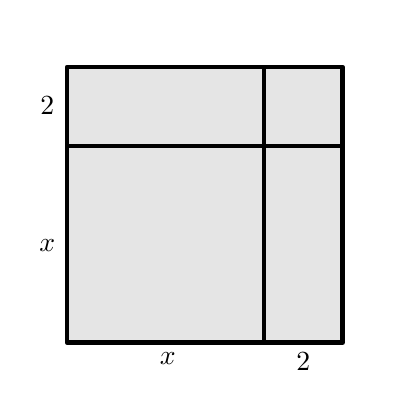
\begin{tikzpicture}[scale=0.5, line cap=round,line join=round,>=triangle 45,x=1.0cm,y=1.0cm]
\clip(-1,-1) rectangle (8,8);
\filldraw[line width=1.6pt,fill=black,fill opacity=0.1] (0,0) -- (5,0) -- (5,5) -- (0,5) -- cycle;
\filldraw[line width=1.6pt,fill=black,fill opacity=0.1] (5,0) -- (7,0) -- (7,5) -- (5,5) -- cycle;
\filldraw[line width=1.6pt,fill=black,fill opacity=0.1] (0,5) -- (5,5) -- (5,7) -- (0,7) -- cycle;
\filldraw[line width=1.6pt,fill=black,fill opacity=0.1] (5,5) -- (7,5) -- (7,7) -- (5,7) -- cycle;
\draw (2.56,0) node[anchor=north] {$x$};
\draw (-0.5,2.87) node[anchor=north] {$x$};
\draw (6,0) node[anchor=north] {$2$};
\draw (-0.5,6.5) node[anchor=north] {$2$};
\end{tikzpicture}

    \end{column}
    \begin{column}{0.6\textwidth}
      \small
      \begin{itemize}
        \item \visible<3->{$x^2$ zien als een vierkant met zijde $x$}
        \item \visible<5->{$4x$ zien als twee rechthoeken}
        \item \visible<7->{Oppervlakte is gelijk aan $5$}
        \item \visible<8->{De figuur vervolledigen}
        \item \visible<10->{Nieuwe oppervlakte is $5+4=9$}
        \item \visible<11->{Zijde is $x+2=+\sqrt{9}$}
      \end{itemize}
      \vspace*{0.75cm}
    \end{column}
  \end{columns}  
\end{frame}


\subsection{Les 4: Kennismaking met tweedimensionale stapelproblemen en het dienbladenprobleem}
\begin{frame}
\frametitle{Les 4: Kennismaking met 2-dimensionale stapelproblemen}
\framesubtitle{Overzicht van de lessen}
\begin{list}{\quad}{}
\item Les 1: Inleiding
\item Les 2: Vullen van vierkanten met kleinere vierkanten en zo tot Perfecte Vierkanten komen
\item Les 3: Puzzelen met vierkanten en rechthoeken om vergelijkingen op te lossen
\item {\color{blue}Les 4: Kennismaking met tweedimensionale stapelproblemen en het dienbladenprobleem}
\item Les 5: Het dienbladenprobleem: experimenteren en effectief berekenen
\item Les 6: Het dienbladenprobleem: berekenen, bewijzen en besluiten
\item Les 7: Kanonskogels stapelen
\item Les 8: Vervolg kanonskogels en het bolstapelprobleem van Kepler
\end{list}
\end{frame}

\subsection{Les 5: Het dienbladenprobleem: experimenteren en effectief berekenen}
\begin{frame}
\frametitle{Les 5: Het dienbladenprobleem}
\framesubtitle{Overzicht van de lessen}
\begin{list}{\quad}{}
\item Les 1: Inleiding
\item Les 2: Vullen van vierkanten met kleinere vierkanten en zo tot Perfecte Vierkanten komen
\item Les 3: Puzzelen met vierkanten en rechthoeken om vergelijkingen op te lossen
\item Les 4: Kennismaking met tweedimensionale stapelproblemen en het dienbladenprobleem 
\item {\color{blue}Les 5: Het dienbladenprobleem: experimenteren en effectief berekenen}
\item Les 6: Het dienbladenprobleem: berekenen, bewijzen en besluiten
\item Les 7: Kanonskogels stapelen
\item Les 8: Vervolg kanonskogels en het bolstapelprobleem van Kepler
\end{list}
\end{frame}

\begin{frame}
\frametitle{Les 4 en 5: Het dienbladenprobleem}
\framesubtitle{Lesdoelstellingen}
\begin{itemize}
\item De leerlingen beseffen dat je een tafel \textbf{niet volledig} kan \textbf{bedekken met cirkels} en dat we daarom op zoek kunnen gaan naar de \textbf{optimale configuratie}, namelijk het hexagonaal rooster.
%\item De leerlingen weten wat een \textbf{voronoicel} is en kunnen hiermee de \textbf{effici\"{e}ntie} van een rooster berekenen.
%\item De leerlingen kunnen de \textbf{oppervlakte} van een driehoek, rechthoek, zeshoek en cirkel berekenen.
\item De leerlingen kunnen a.d.h.v. een geogebra-applet of door te experimenteren met jetons of munten de \textbf{effici\"{e}ntie van dienbladen bepalen}.
\item De leerlingen kunnen de effici\"{e}ntie voor eenvoudige voorbeelden \textbf{uitrekenen}.
\item De leerlingen kunnen in groepjes \textbf{samenwerken}.
\item De leerlingen ontwikkelen \textbf{meetkundig inzicht}.
\item De leerlingen kunnen vanuit een figuur meetkundig inzicht verwerven en hierdoor \textbf{problemen vereenvoudigen}.
\item De leerlingen kunnen de meetkundige interpretatie van de \textbf{goniometrische formules} functioneel gebruiken, i.h.b. voor projecties.
\end{itemize}
\end{frame}

\begin{frame}
\frametitle{Les 4 en 5: Het dienbladenprobleem}
\framesubtitle{Didactische wenken}

\begin{enumerate}
	\item Onderwijsleergesprek
	\begin{itemize}
	\item Kennismaking met tweedimensionale stapelproblemen a.d.h.v. een bundeltje met vragen en opdrachten
\end{itemize}
	
	\item In groepjes werken en experimenteren 
	\begin{itemize}
	\item Geogebra-applets
	\item Jetons of munten en karton
	\item Effectief berekenen
\end{itemize}

  \item Onderwijsleergesprek
  \begin{itemize}
	\item Gevonden resultaten samen overlopen
	\item Enkele voorbeelden klassikaal maken
\end{itemize}
\end{enumerate}
\end{frame}


\begin{frame}\frametitle{Tweedimensionale Stapelproblemen}
\framesubtitle{Algemeen}
\begin{block}{Vraag}
Hebben we ook 100\% effici�ntie als we een oneindig vlak zouden betegelen met cirkels?
\end{block}
\pause
%\begin{figure}[h]
 % \centering
 % \subfloat[]{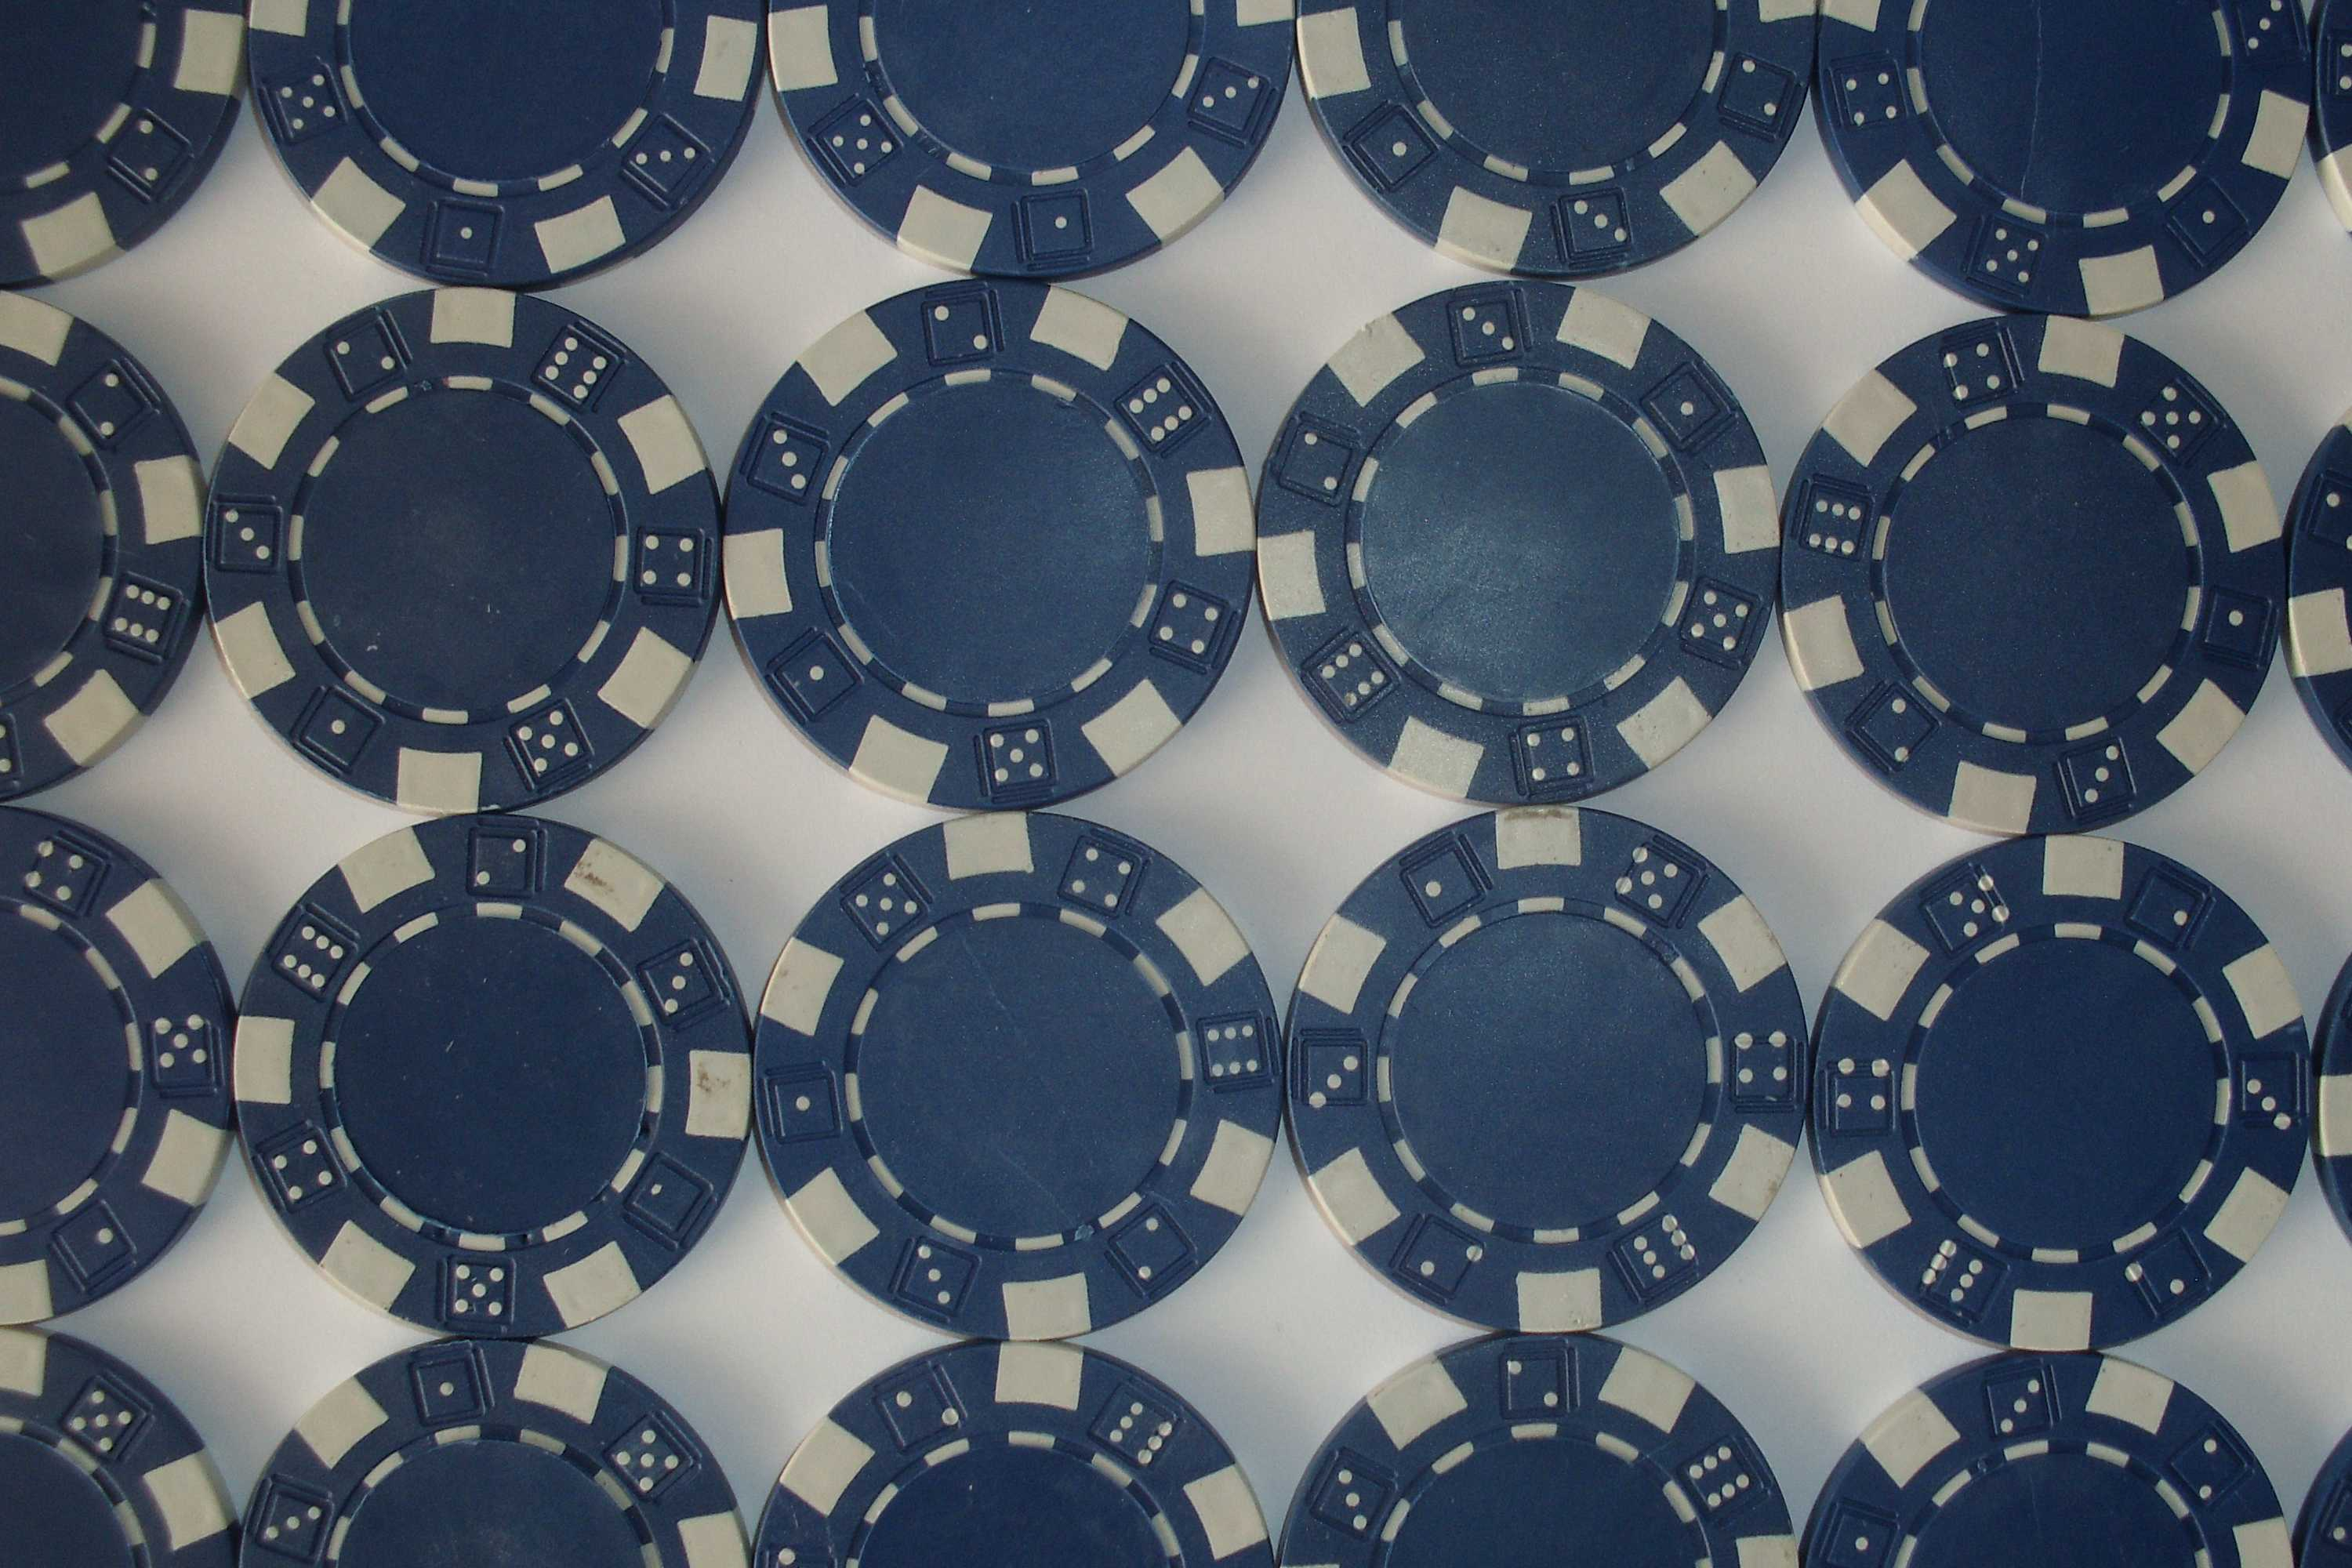
\includegraphics[height= 4cm]{jetons_sqr}\label{js}}\qquad
 % \subfloat[]{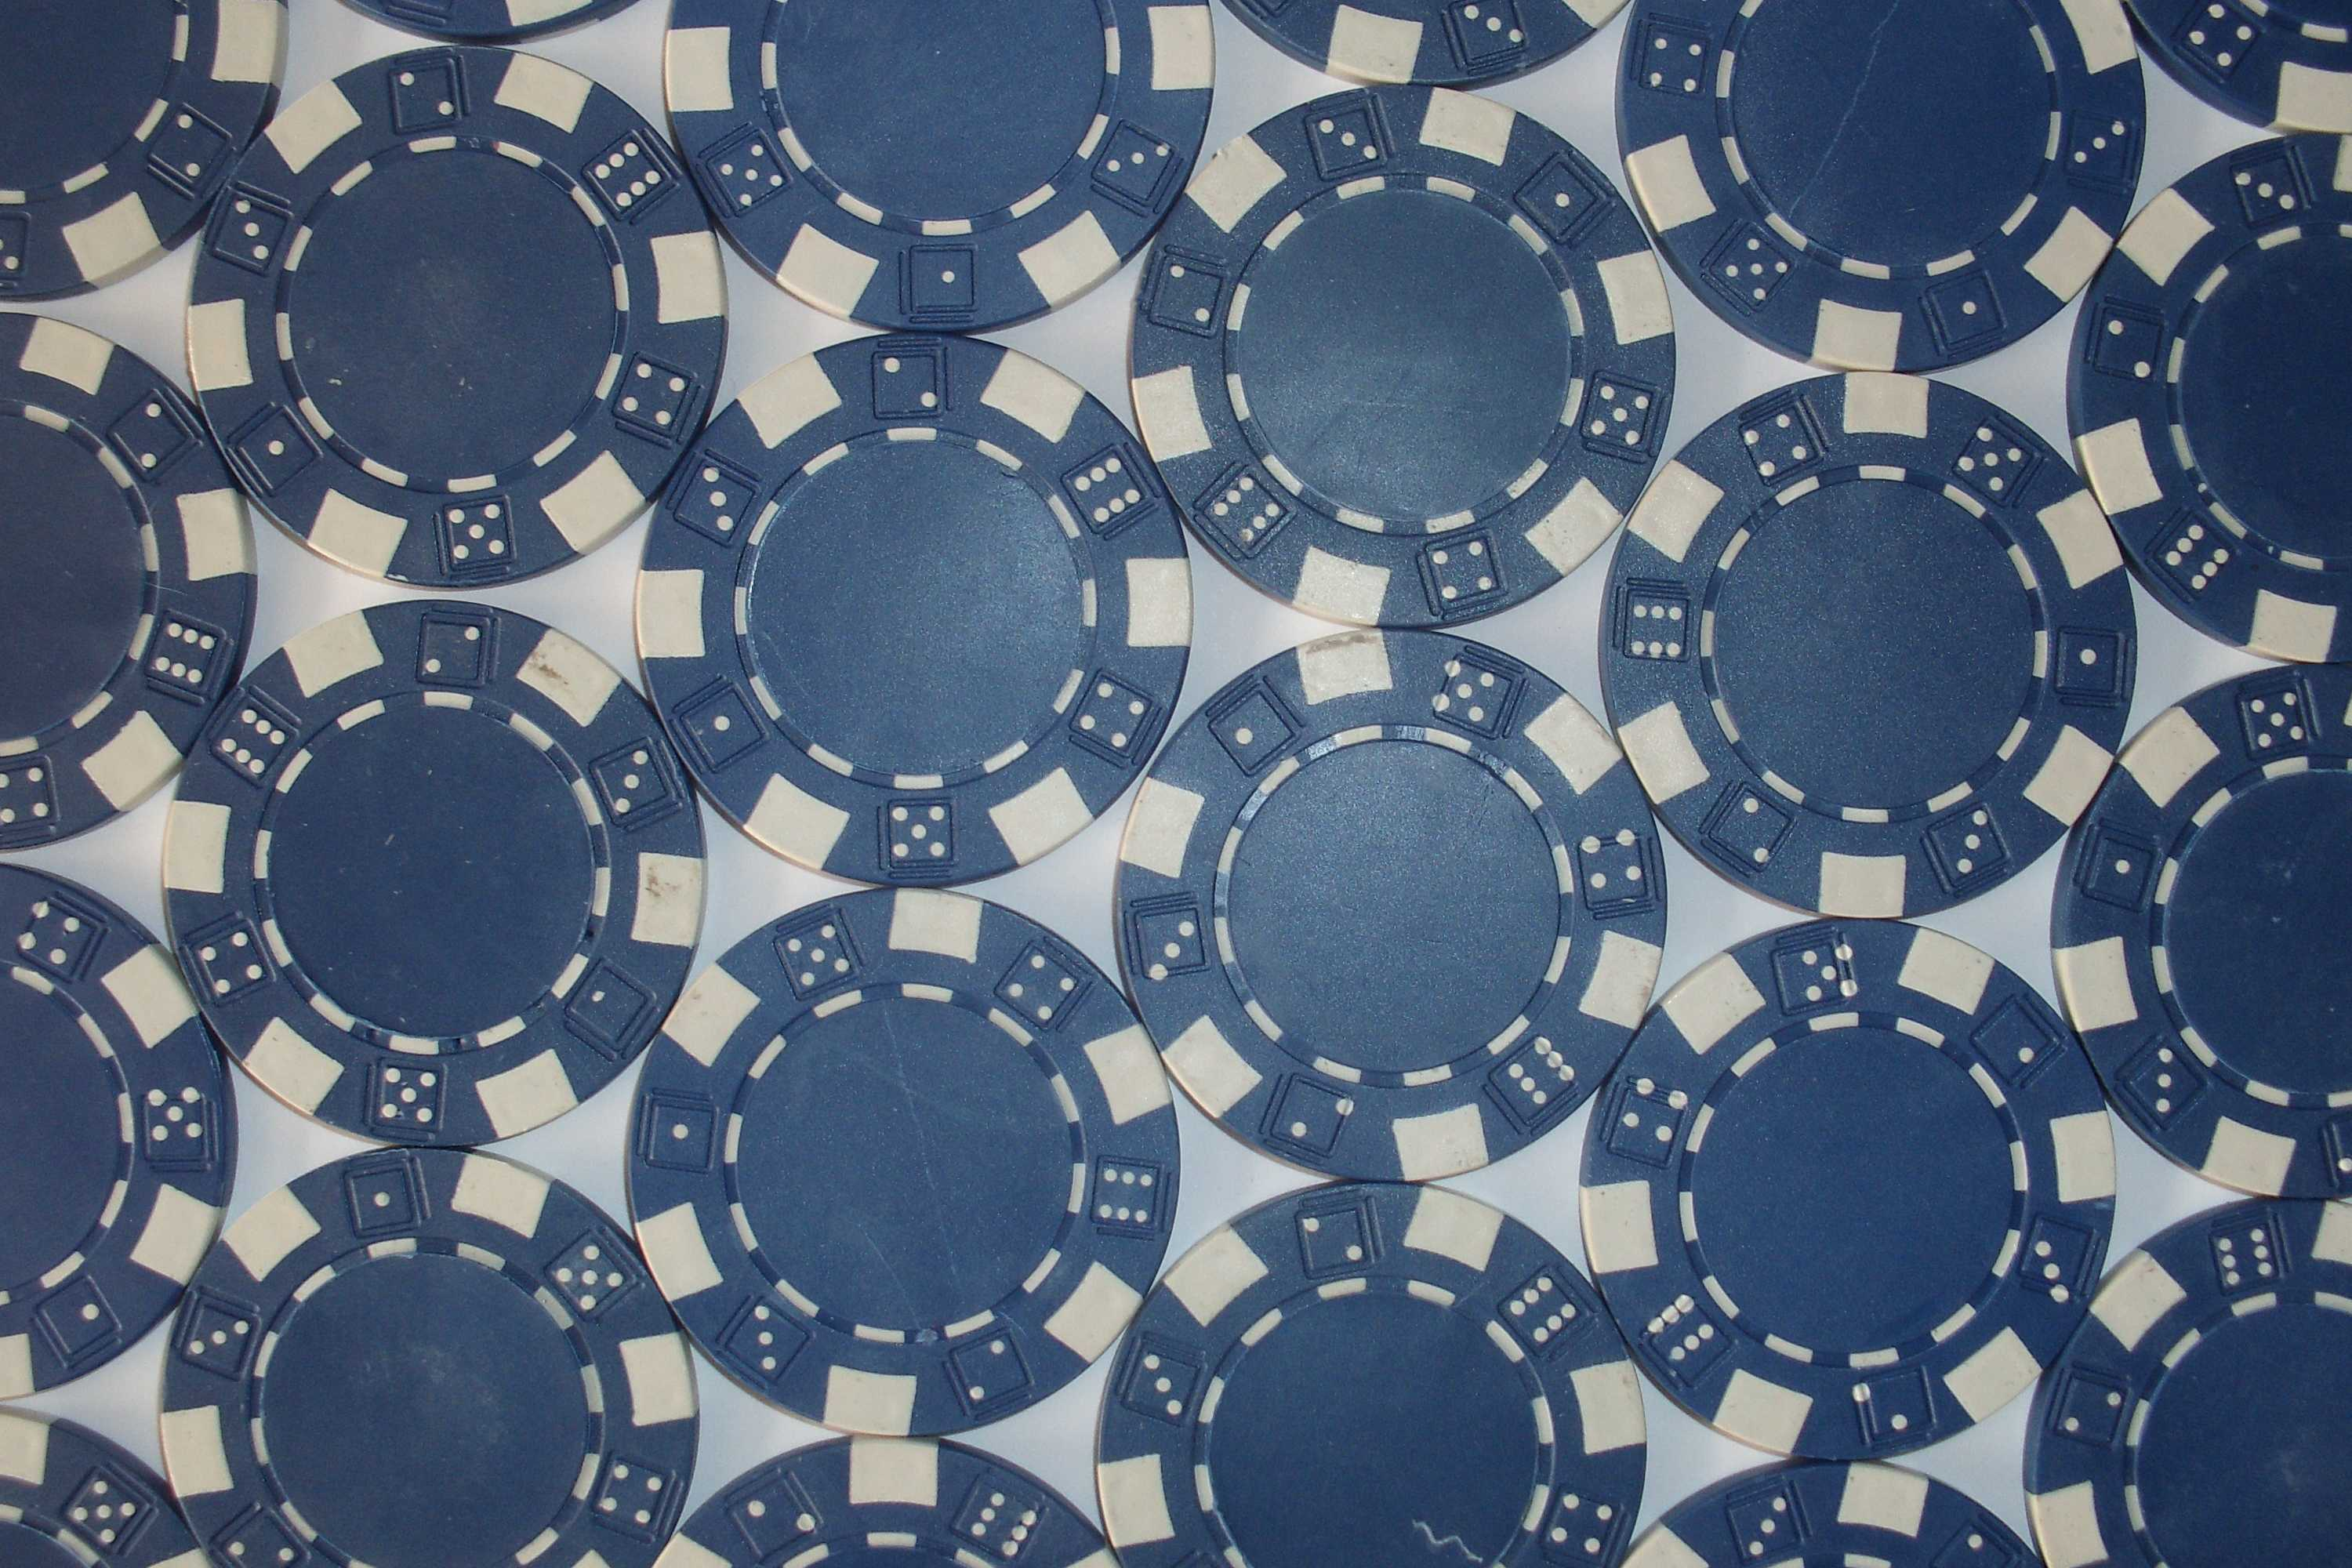
\includegraphics[height=4cm]{jetons_hex}\label{jh}}
 % \caption{Vierkante en hexagonale rangschikking met pokerjetons en hun voronoicellen.}  
%\end{figure}
\begin{columns}
        \begin{column}{0.4\textwidth}
    \begin{block}{Opdracht}
Probeer cirkels (munten, flippo's, pokerjetons ...) eens zodanig op een tafel te leggen dat er zo weinig mogelijk ruimte tussen de cirkels overblijft.
\end{block}
\end{column}
\begin{column}{0.4\textwidth}
      \only<3>{\begin{figure}[h]
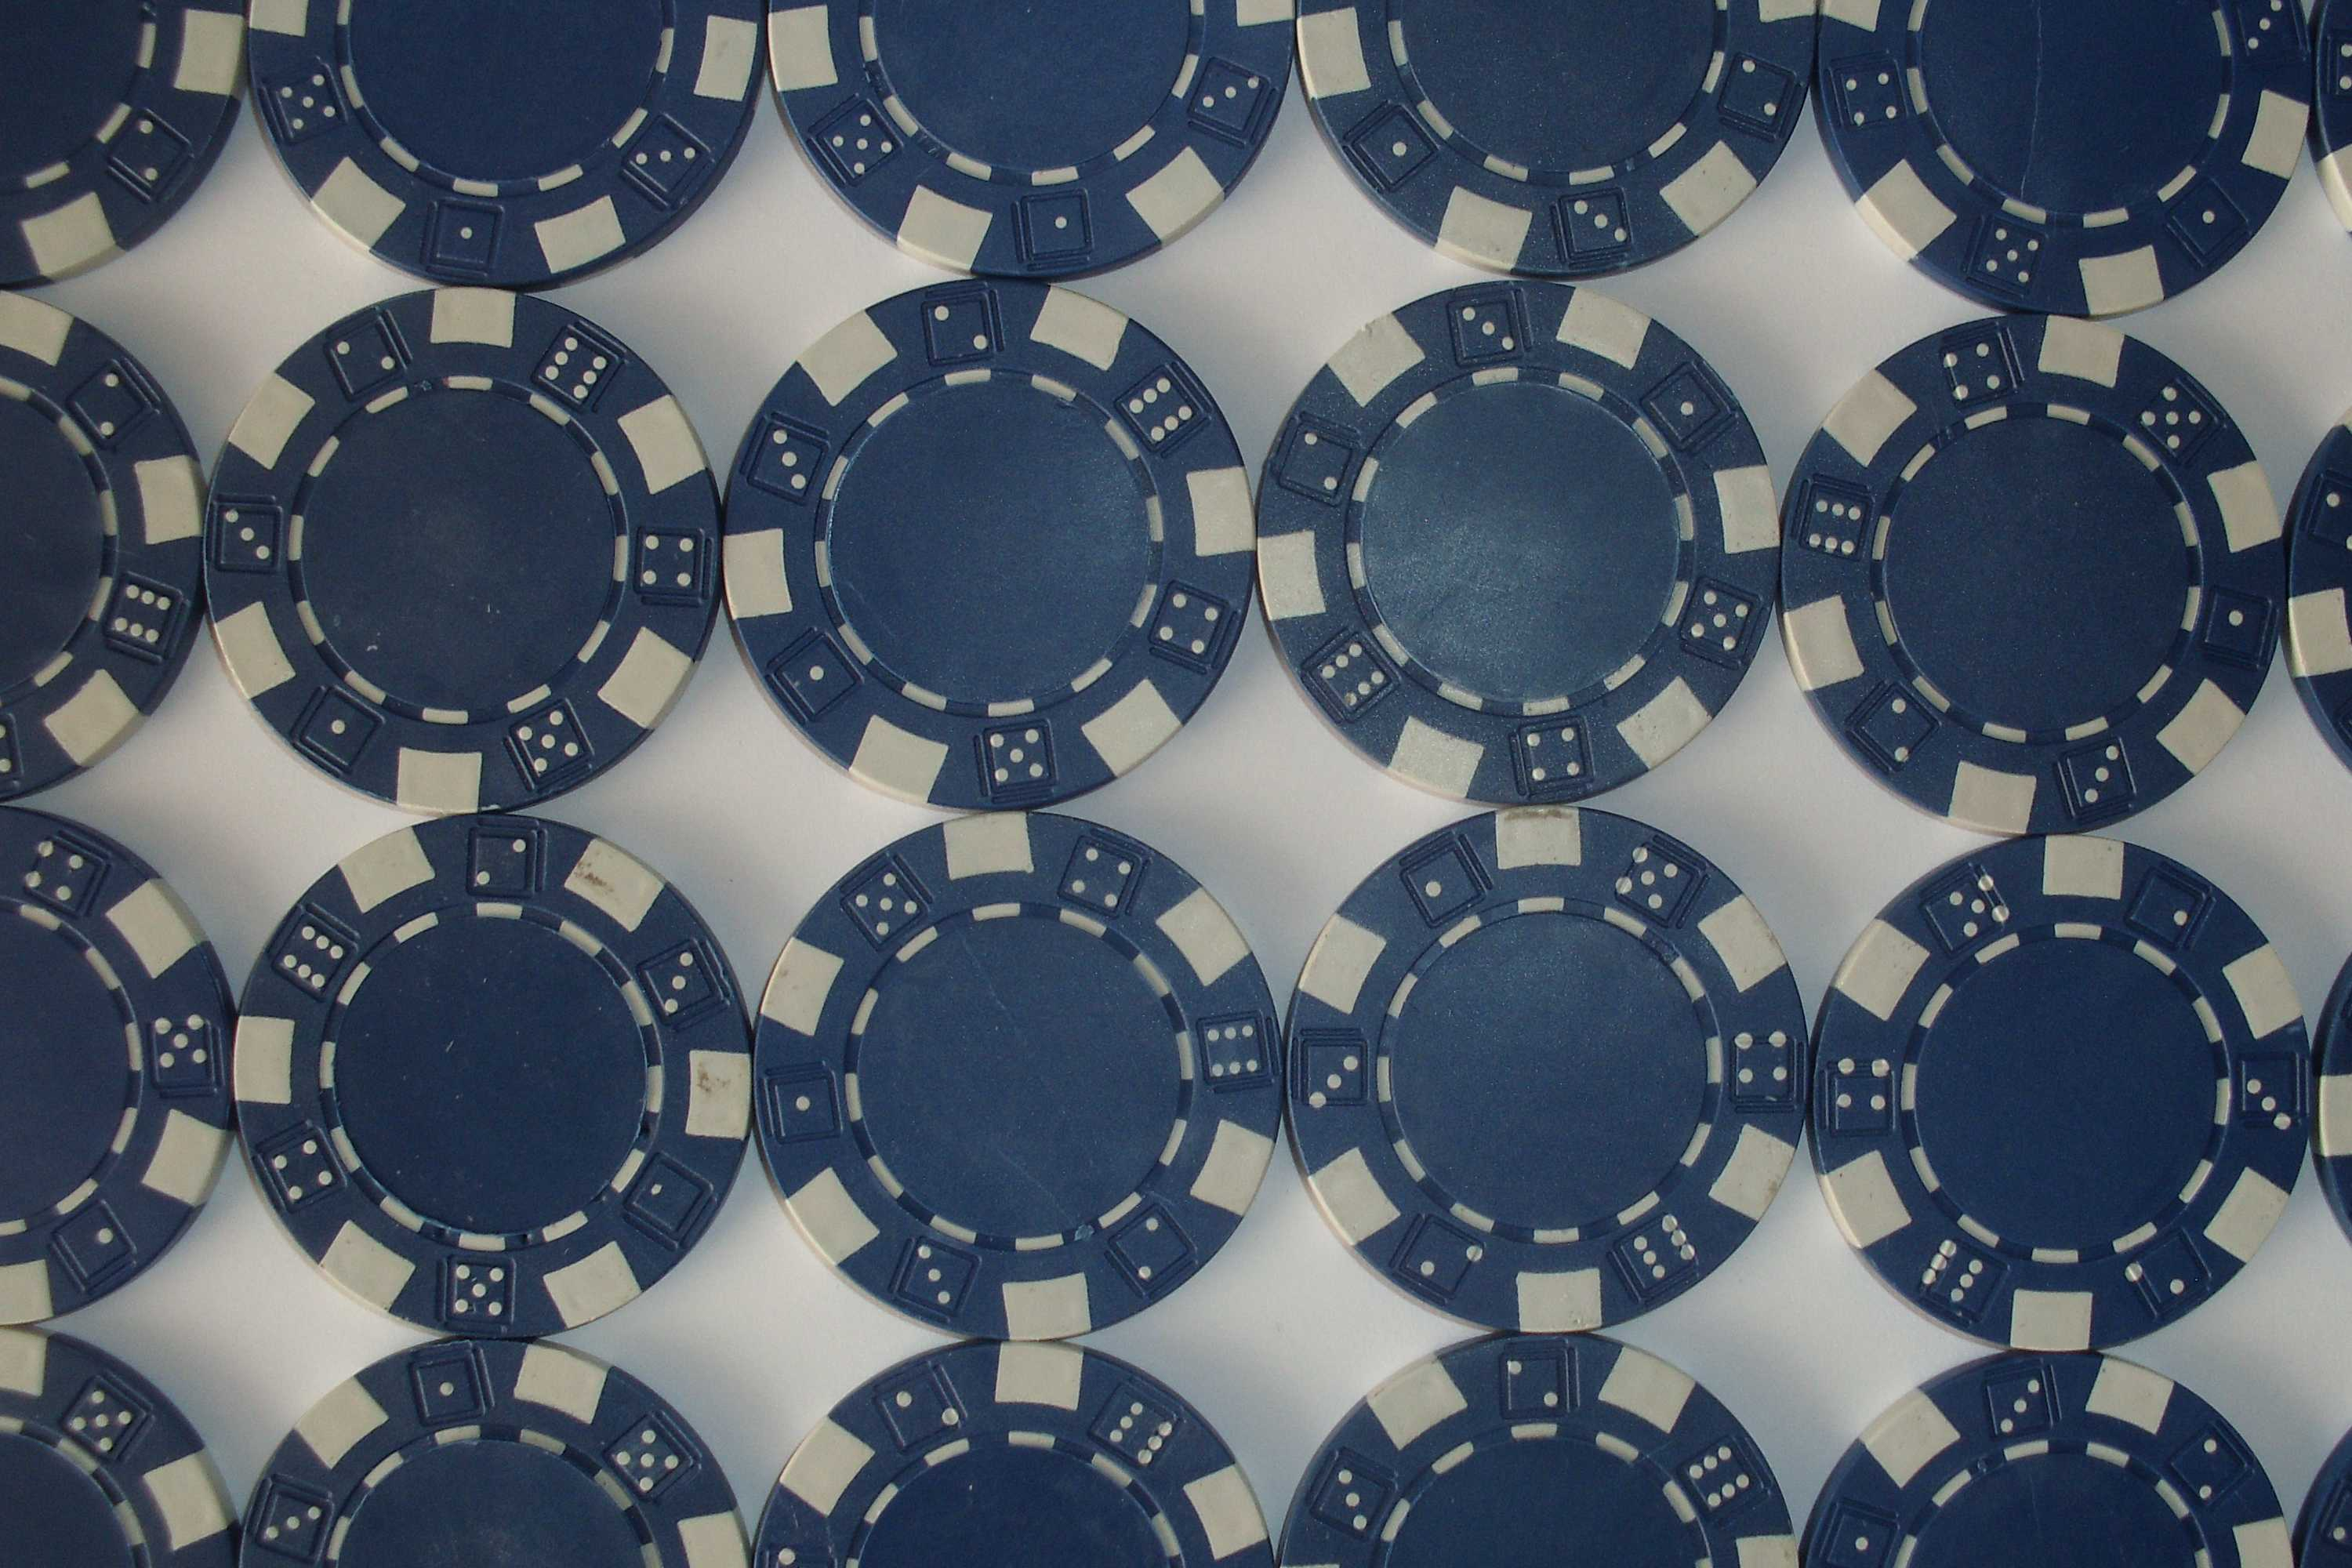
\includegraphics[width=\columnwidth]{jetons_sqr}
\end{figure}}
      \only<4>{\begin{figure}[h]
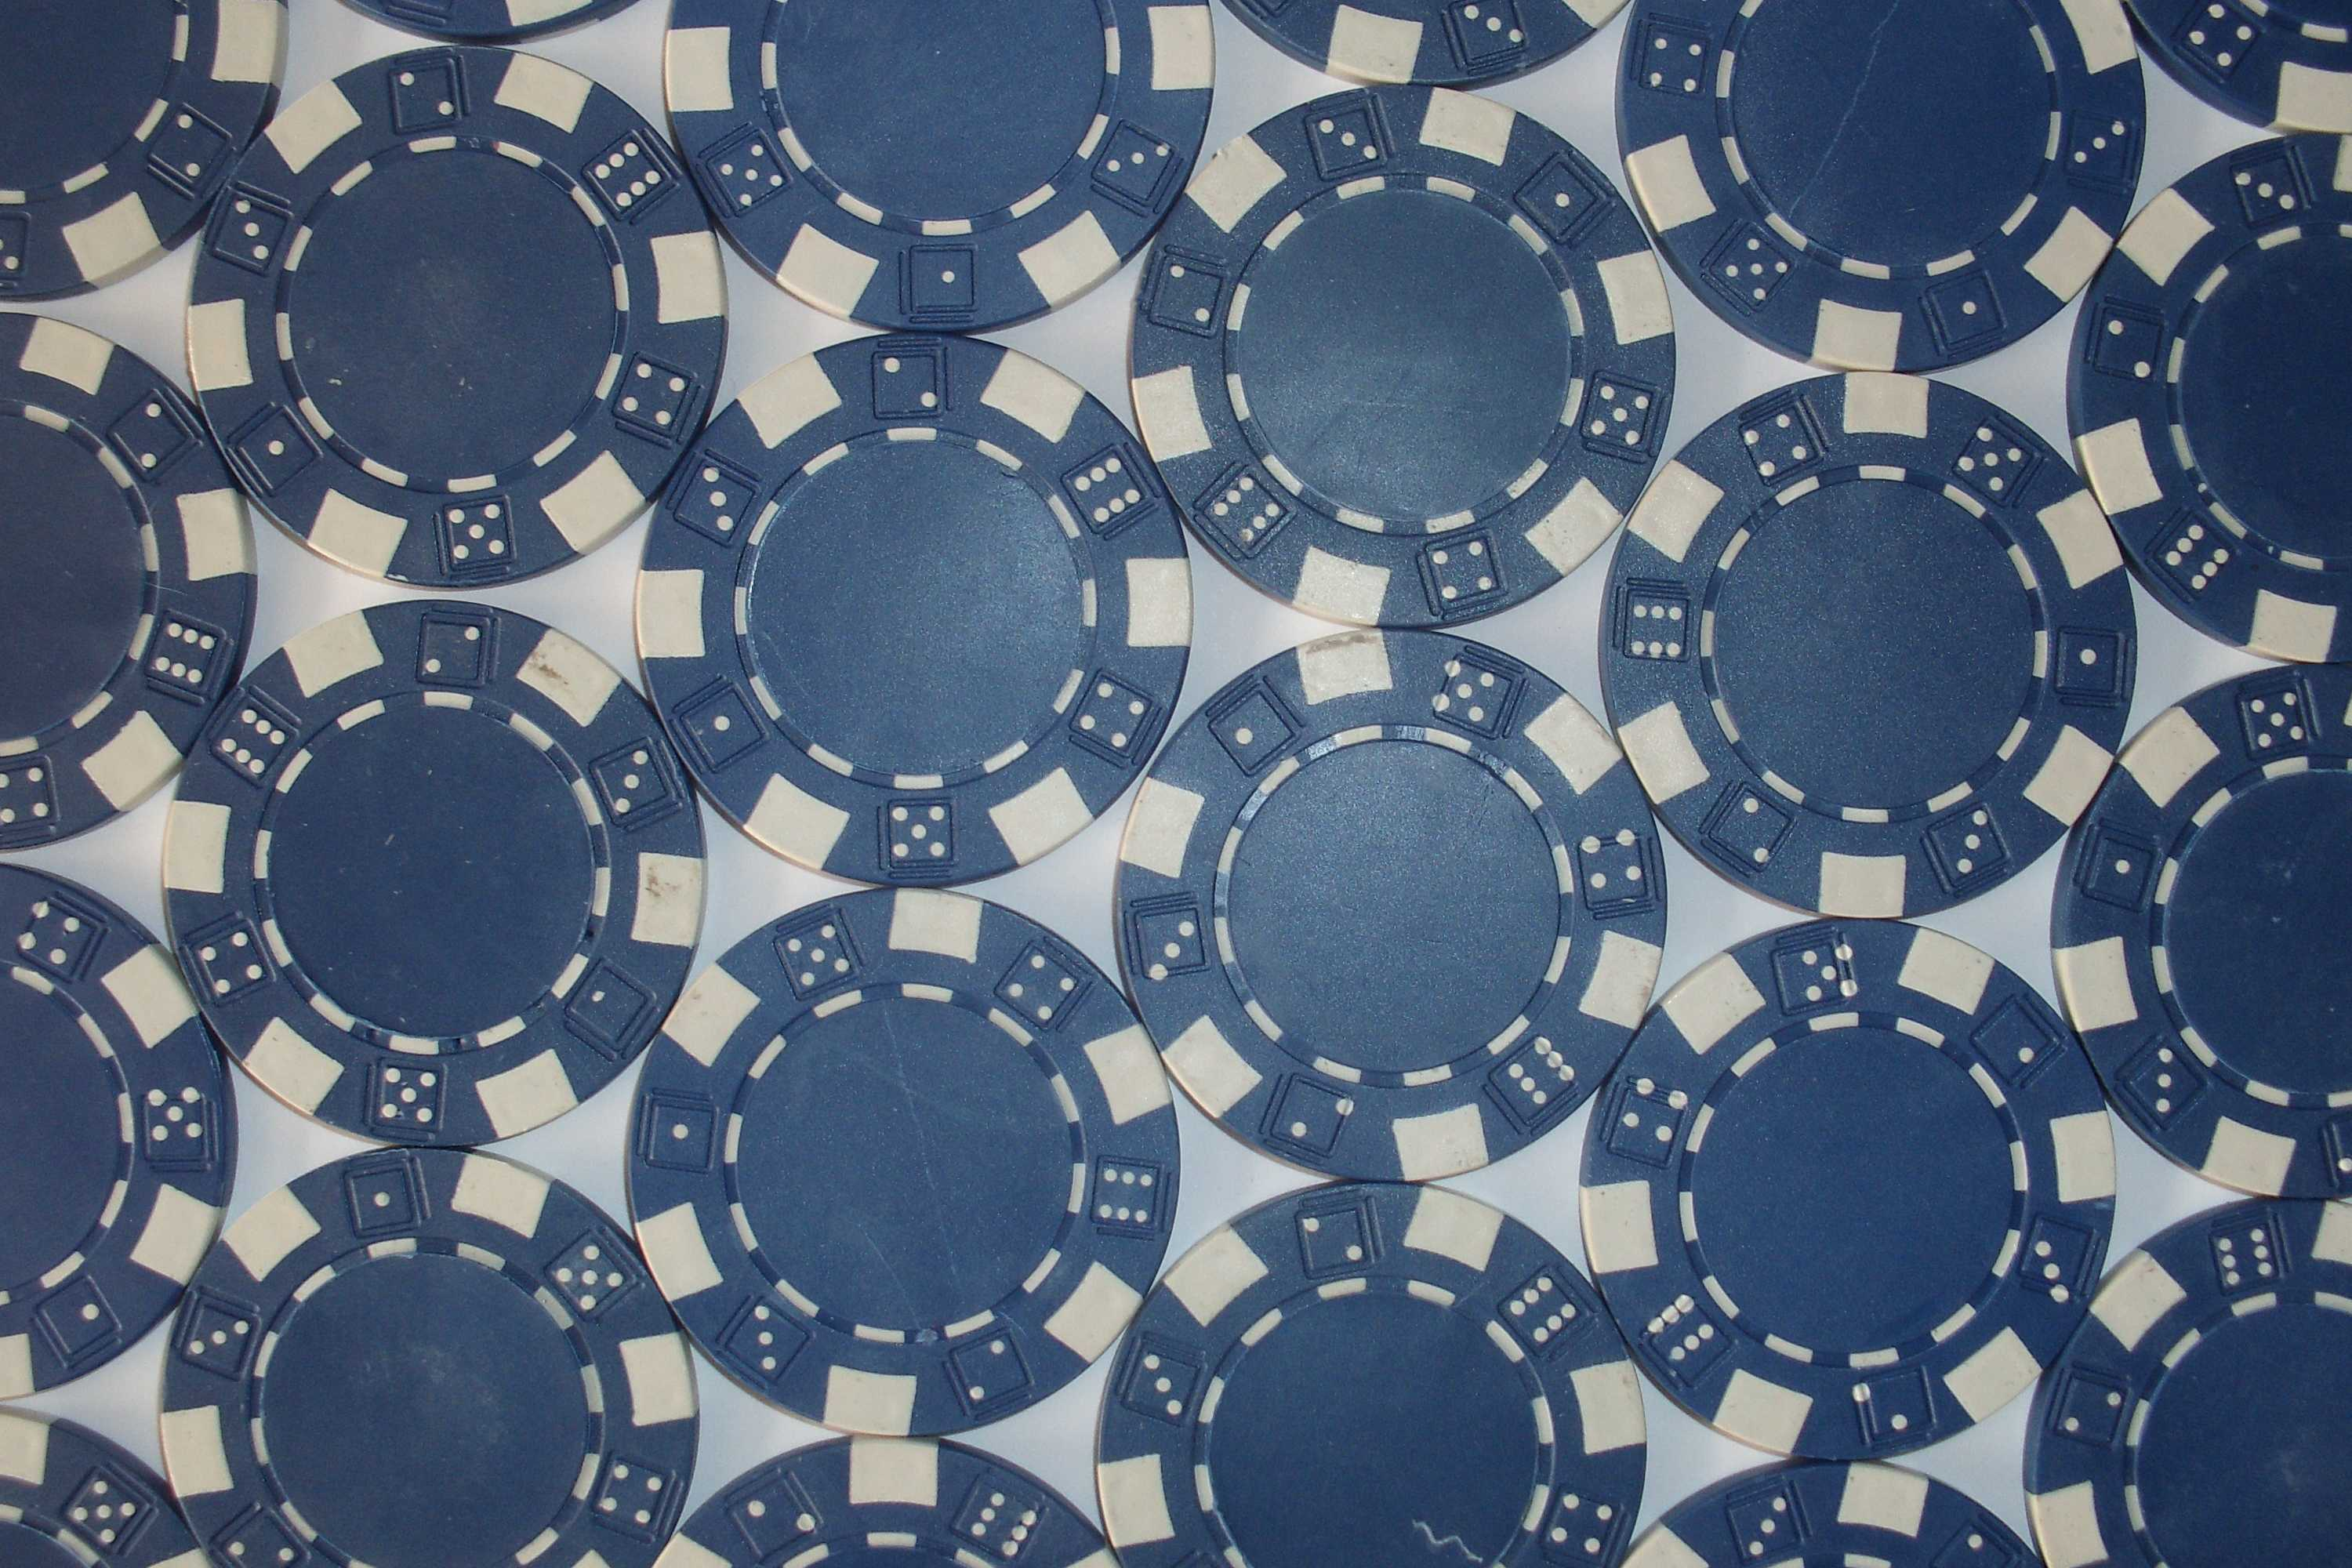
\includegraphics[width=\columnwidth]{jetons_hex}
\end{figure}}
      \only<5>{\begin{itemize}
	\item Hexagonaal rooster
	\item Meest effici�nt
	\item Bewezen door Axel Thue
\end{itemize}}
    \end{column}

  \end{columns}  

\end{frame}

\begin{frame}\frametitle{Tweedimensionale stapelproblemen}
\begin{block}{Voronoicel}
De {\bf Voronoicel} van een cirkel is de verzameling van alle punten die dichter bij het middelpunt van deze cirkel liggen dan bij het middelpunt van elke andere cirkel in de schikking.
\end{block}
\end{frame}


\begin{frame}
  \frametitle{Tweedimensionale stapelproblemen}
  \begin{block}{Voronoicel}
  De {\bf Voronoicel} van een cirkel is de verzameling van alle punten die dichter bij het middelpunt van deze cirkel liggen dan bij het middelpunt van elke andere cirkel in de schikking.
  \end{block}
  \begin{columns}
    \begin{column}{0.4\textwidth}
      \begin{block}{Vraag}
      Hoe ziet de Voronoicel eruit bij een vierkante rangschikking? Hoe ziet de Voronoicel eruit bij de hexagonale rangschikking?
      \end{block}
    \end{column}
    \begin{column}{0.4\textwidth}
      \only<2>{
        \begin{figure}[h]
        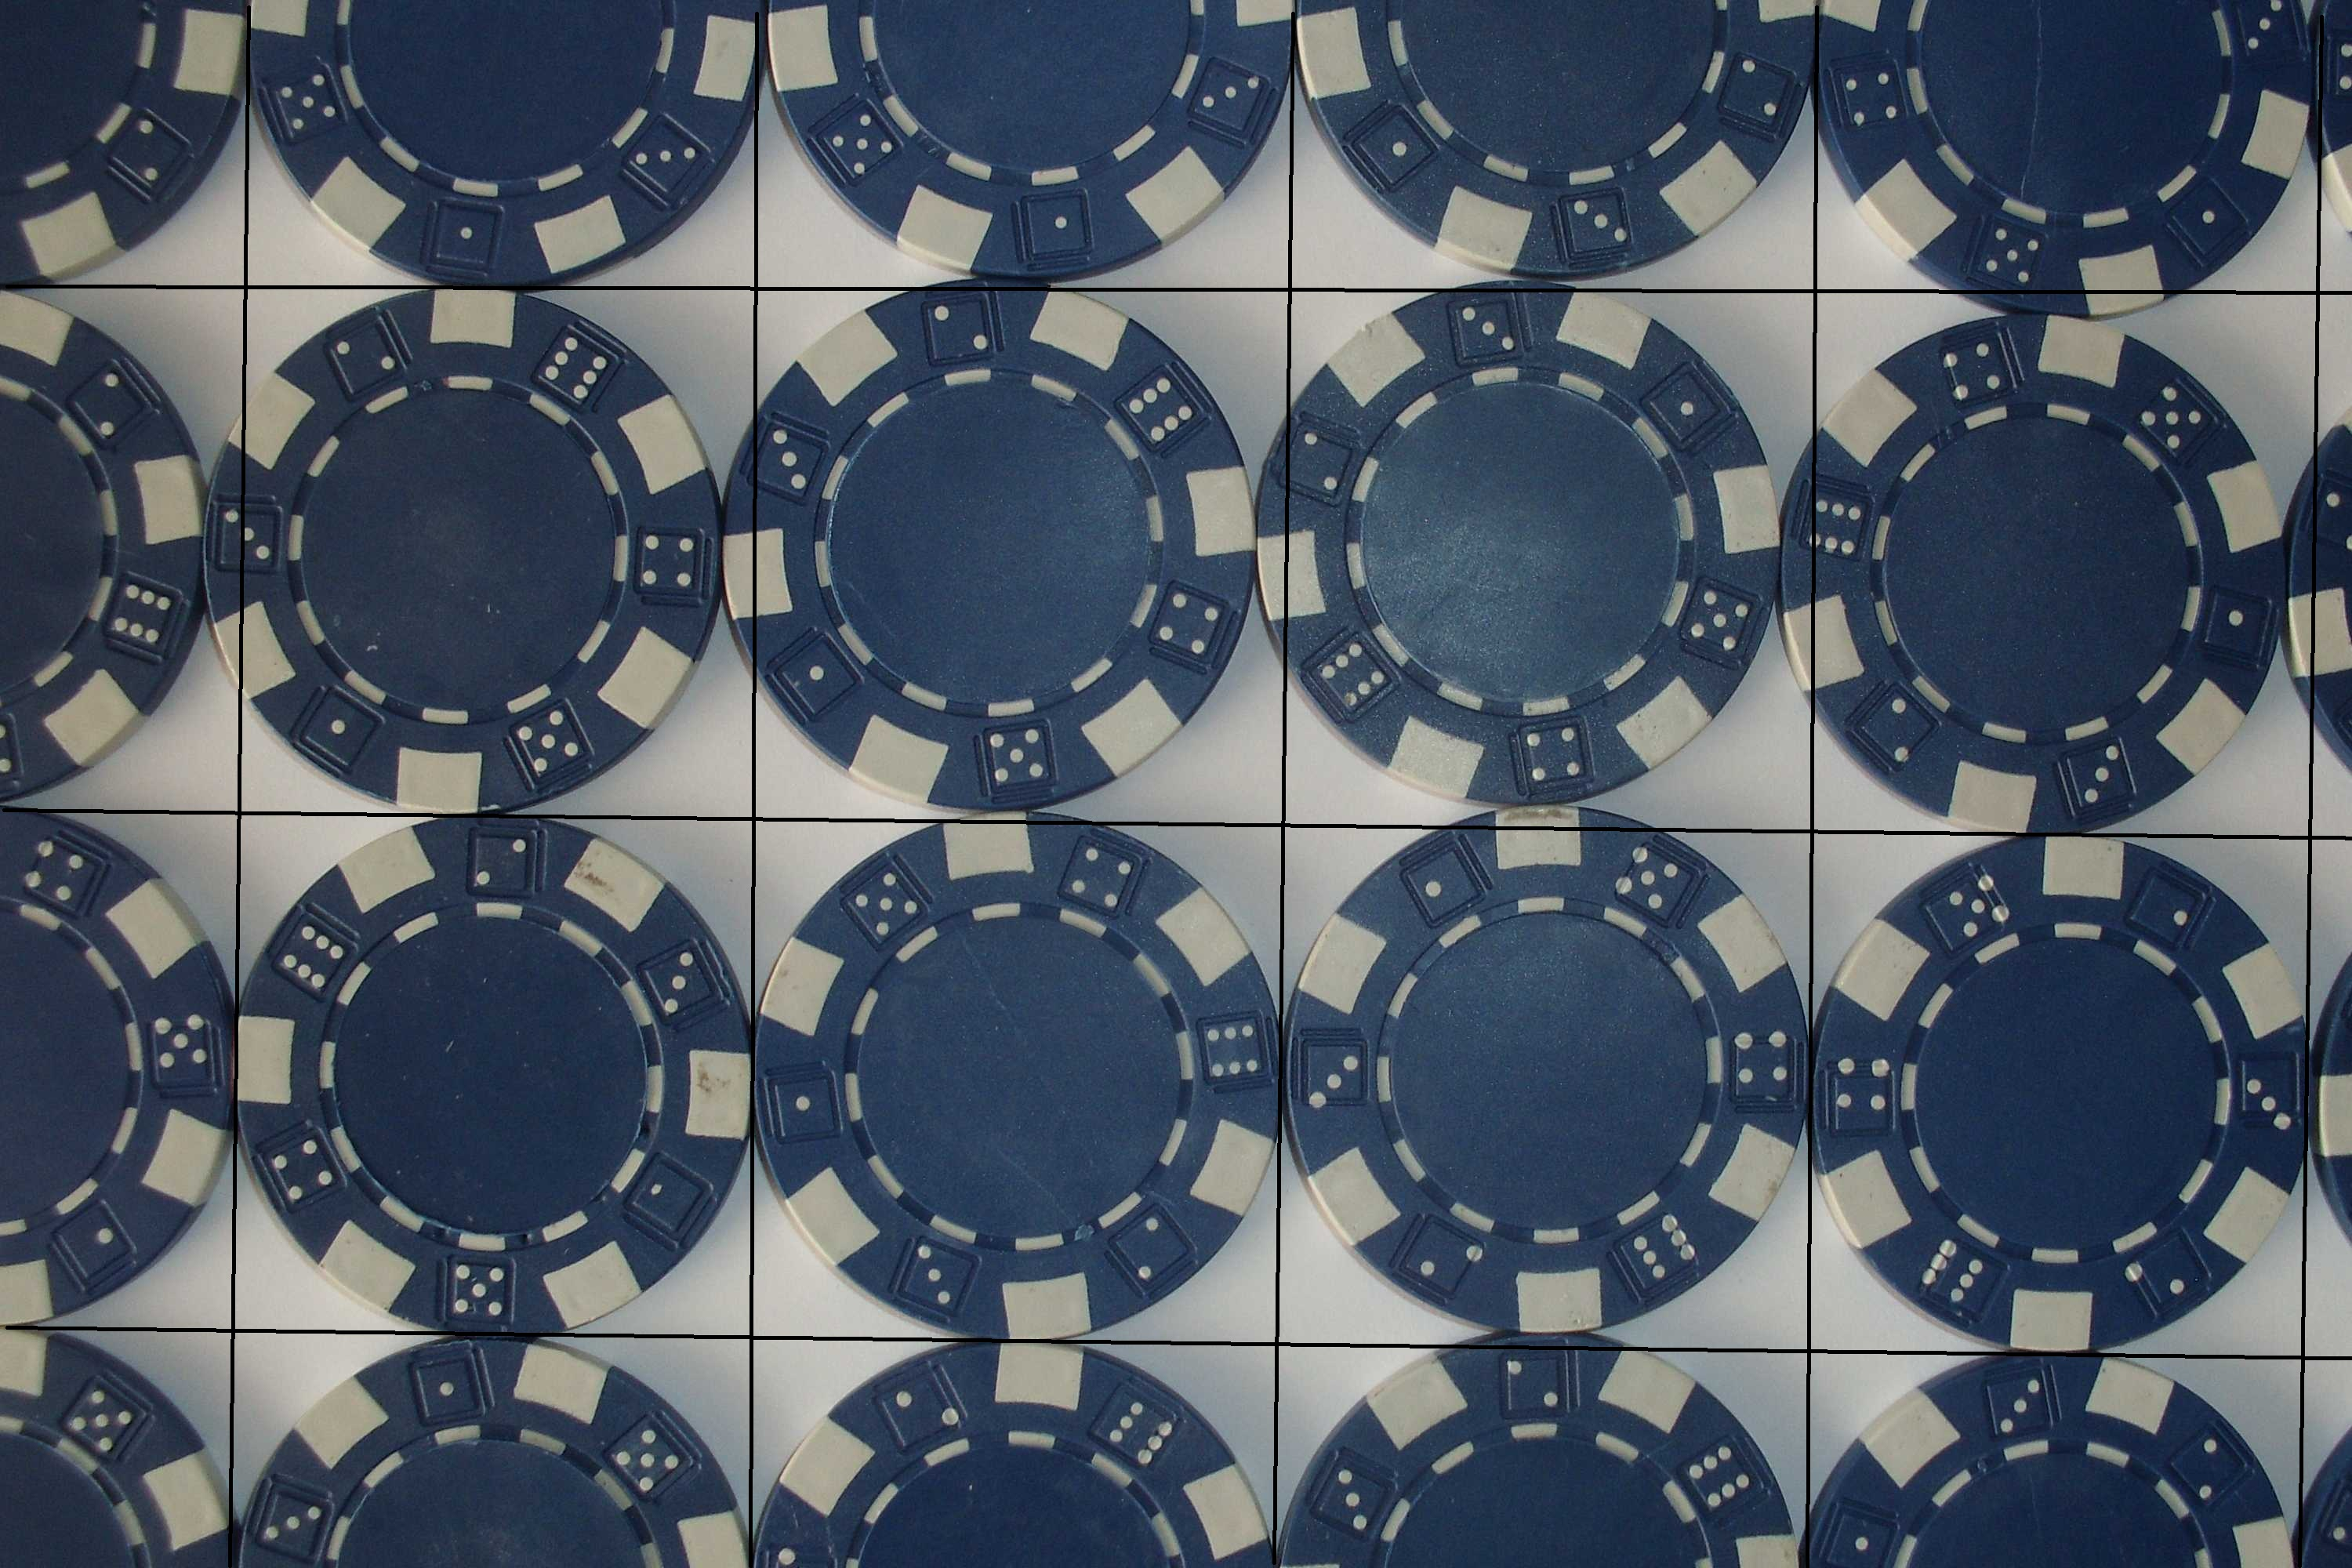
\includegraphics[width=\columnwidth]{voronoi_sqr}
        \end{figure}
      }
      \only<3>{
        \begin{figure}[h]
        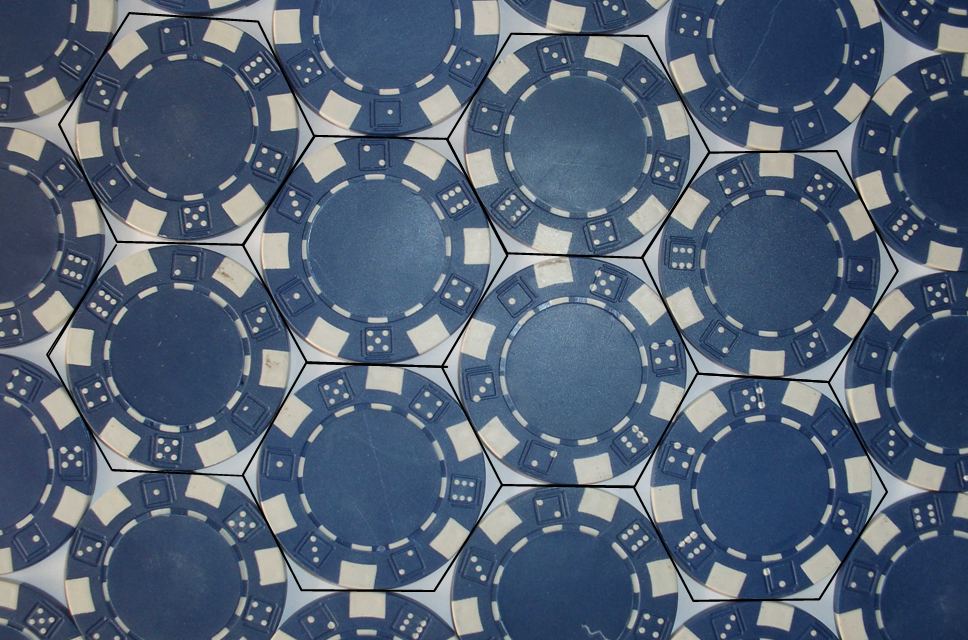
\includegraphics[width=\columnwidth]{voronoi_hex}
        \end{figure}
      }
    \end{column}
  \end{columns}  
%Omdat in het tweede deel van de les en ook de volgende les de leerlingen zelf de effici�ntie zullen moeten berekenen is het goed om dit al eens klassikaal te doen.
%\begin{block}{Vraag}
%Hoe kan je de effici�ntie berekenen aan de hand van zo'n Voronoicel?
%\end{block}
\end{frame}

\begin{frame}\frametitle{Tweedimensionale stapelproblemen}
\framesubtitle{Voronoicellen}
\begin{block}{Opdracht}
Bereken voor de vierkante en de hexagonale rangschikking de effici�ntie.
\end{block}
\pause
\begin{columns}
\begin{column}{0.6\textwidth}     
\begin{enumerate}
	\item Vierkante rangschikking: \\
 Effici�ntie = $\frac{\pi}{4}=0,78538...$
 \pause
	\item Hexagonale rangschikking:\\
	Effici�ntie = $\frac{\pi}{\sqrt{12}}=0.90689$
	%Dit is ook de meest effici�nte!!! -> Axel Thue heeft dit aangetoond en we geven in de cursus ook een kleine schets van het bewijs.
\end{enumerate}
\end{column}
\begin{column}{0.4\textwidth}     
     \begin{figure}[h]
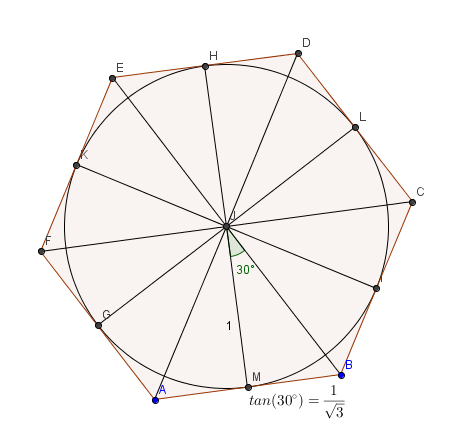
\includegraphics[width=\columnwidth]{hexagon}
\end{figure}
   \end{column}
\end{columns}  
\end{frame}

\begin{frame}
\frametitle{Tweedimensionale stapelproblemen}
\framesubtitle{Dienbladenprobleem: Opdracht}

Een fabrikant wil dienbladen voor een bepaalde aantal glazen of blikjes. Omdat de fabrikant ruimdenkend is, wil hij niet enkel de traditionele cirkelvormige dienbladen uitproberen, maar ook driehoekige, rechthoekige of zeshoekige dienbladen. 
\pause
\begin{block}{Opdracht}Bepaal nu voor een gegeven aantal glazen of blikjes we welk soort dienblad willen maken en wat juist de effici�ntie is%, m.a.w. hoeveel procent van het dienblad dat gevuld zal zijn
. Controleer dit voor dienbladen in de vorm van een cirkel, een gelijkzijdige driehoek, een rechthoek en een regelmatige zeshoek.
\end{block}
\end{frame}

\begin{frame}
\frametitle{Tweedimensionale stapelproblemen}
\framesubtitle{Dienbladenprobleem: Experimenteren}


\begin{table}[h]
\centering
\small
\begin{tabular}{l||c|c|c|c}
Aantal / vorm & cirkelvormig & driehoekig & rechthoekig& zeshoekig\\\hline\hline
1&&&&\\\hline
2&&&&\\\hline
3&&&&\\\hline
4&&&&\\\hline
5&&&&\\\hline
6&&&&\\\hline
7&&&&\\\hline
8&&&&\\\hline
9&&&&\\\hline
10&&&&\\\hline
11&&&&\\\hline
12&&&&\\\hline
13&&&&\\\hline
...&&&&\\
\end{tabular}
\end{table}
\end{frame}



\begin{frame}
  \frametitle{Tweedimensionale stapelproblemen}
  \framesubtitle{Dienbladenprobleem: Experimenteren}
  Hoe pakken we dit aan?
  De klas wordt verdeeld in groepen die (al dan niet gesplitst)
  \begin{enumerate}
	  \item Experimenteren a.d.h.v. Geogebra-applets:
	  \begin{itemize}
      \item \href{http://wiskunde.github.com/V3/cirkelvormigdienblad_applet.html}{Cirkelvormig}
      \item \href{http://wiskunde.github.com/V3/Driehoekigdienblad_applet.html}{Driehoekig}
      \item \href{http://wiskunde.github.com/V3/Rechthoekigdienblad_applet.html}{Rechthoekig}
      \item \href{http://wiskunde.github.com/V3/zeshoekigdienblad_applet.html}{Zeshoekig}
    \end{itemize}
	  \item Experimenteren a.d.h.v. pokerjetons, karton en liniaal:
	  \begin{itemize}
    	\item Driehoekig
    	\item Rechthoekig
    \end{itemize}
  \end{enumerate}
\end{frame}


\begin{frame}
\frametitle{Tweedimensionale stapelproblemen}
\framesubtitle{Dienbladenprobleem: Experimenteren en berekenen}

\begin{figure}[h]
\centering
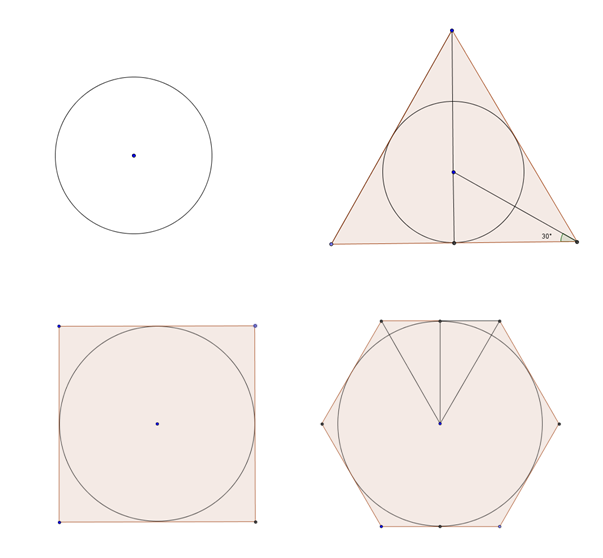
\includegraphics[height=5cm]{1munten}
\caption{De dienbladen voor 1 munt.}
\label{2munt}
\end{figure}

\end{frame}


\begin{frame}
\frametitle{Tweedimensionale stapelproblemen}
\framesubtitle{Dienbladenprobleem: Experimenteren en berekenen}

\begin{figure}[h]
\centering
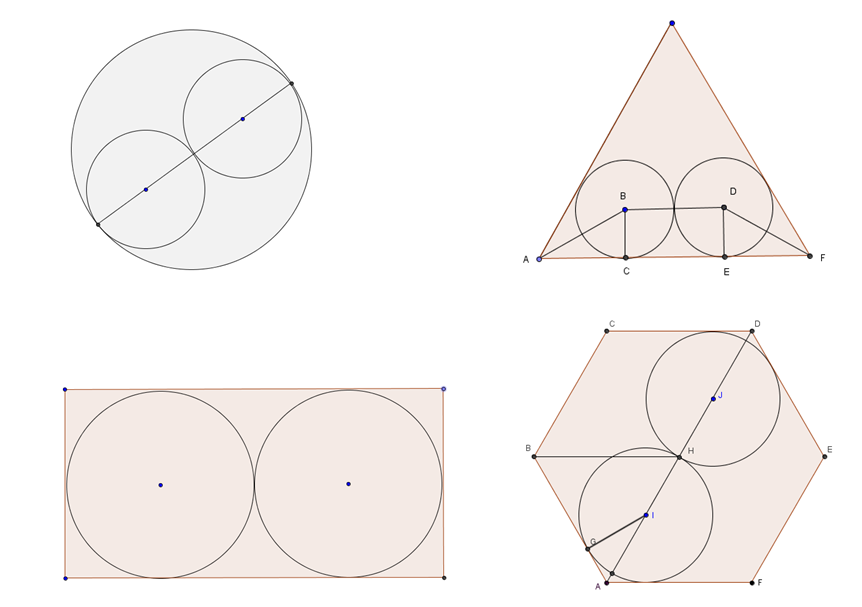
\includegraphics[height=5cm]{2munten}
\caption{De dienbladen voor 2 munten.}
\label{2munt}
\end{figure}

\end{frame}


\begin{frame}
\frametitle{Tweedimensionale stapelproblemen}
\framesubtitle{Dienbladenprobleem: Experimenteren en berekenen}

\begin{figure}[h]
\centering
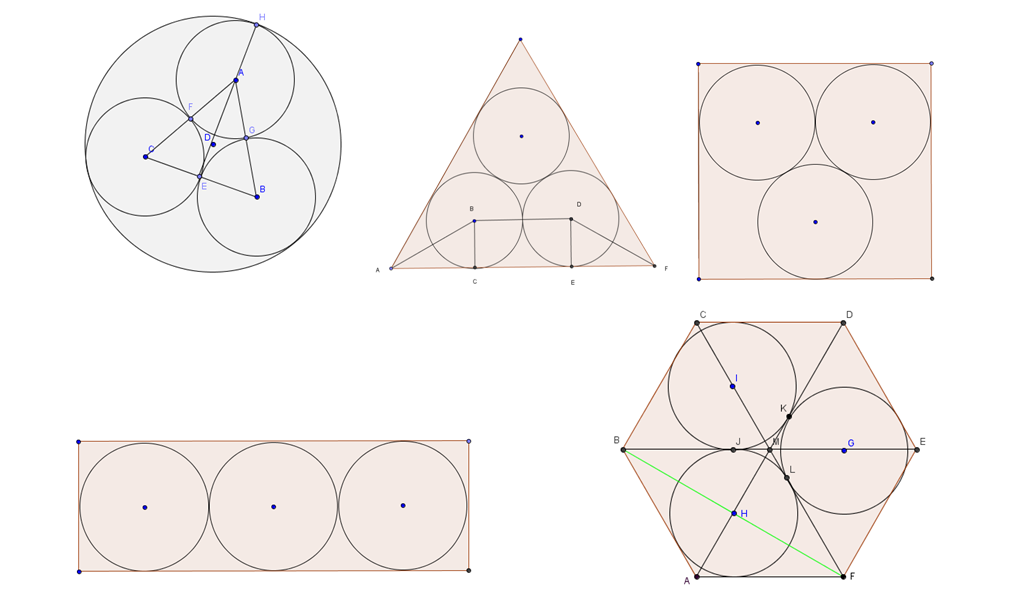
\includegraphics[height=5cm]{3munten}
\caption{De dienbladen voor 3 munten.}
\label{2munt}
\end{figure}

\end{frame}



\subsection{Les 6: Het dienbladenprobleem: berekenen, bewijzen en besluiten}
\begin{frame}
\frametitle{Les 6: Het dienbladenprobleem {\small (vervolg)}}
\framesubtitle{Overzicht van de lessen}
\begin{list}{\quad}{}
\item Les 1: Inleiding
\item Les 2: Vullen van vierkanten met kleinere vierkanten en zo tot Perfecte Vierkanten komen
\item Les 3: Puzzelen met vierkanten en rechthoeken om vergelijkingen op te lossen
\item Les 4: Kennismaking met tweedimensionale stapelproblemen en het dienbladenprobleem 
\item Les 5: Het dienbladenprobleem: experimenteren en effectief berekenen
\item {\color{blue}Les 6: Het dienbladenprobleem: berekenen, bewijzen en besluiten}
\item Les 7: Kanonskogels stapelen
\item Les 8: Vervolg kanonskogels en het bolstapelprobleem van Kepler
\end{list}
\end{frame}

\begin{frame}
\frametitle{Les 6: Het dienbladenprobleem {\small (vervolg)}}
\framesubtitle{Lesdoelstellingen}
\begin{itemize}
\item De leerlingen beseffen dat men uit experimenteren belangrijke informatie kan halen en \textbf{beseffen ook het belang van bewijzen}.
\item De leerlingen kunnen aan de hand van een \textbf{stappenplan} het bewijs zelf verwerven.
\item De leerlingen kunnen de \textbf{effici\"{e}ntie} van ingewikkelde configuraties berekenen.
\item De leerlingen kunnen vorige berekeningen gebruiken om ingewikkelde configuraties te \textbf{vereenvoudigen}.
\item De leerlingen kunnen uit experimentele resultaten \textbf{conclusies} trekken over de meest effici\"{e}nte dienbladen, en kunnen ook (mogelijke) verklaringen geven.
\end{itemize}
\end{frame}


\begin{frame}
\frametitle{Les 6: Het dienbladenprobleem {\small (vervolg)}}
\framesubtitle{Didactische wenken}

\begin{enumerate}
	\item Onderwijsleergesprek
	\begin{itemize}
	\item Doel van deze les en de opdracht laten aanvoelen en uitleggen
\end{itemize}
	
	\item In groepjes werken
	\begin{itemize}
	\item A.d.h.v. een bundeltje met vragen en opdrachten iets bewijzen waarbij ze het stappenplan kunnen volgen
	\item M.b.v. een (zelfgemaakte) figuur het bewijs visueel maken
	\item Experimenteren, tekenen en berekenen
	% Leerkracht helpt waar nodig en loopt rond!!
\end{itemize}

  \item Onderwijsleergesprek
  \begin{itemize}
  \item Moeilijkheden en problemen in het bewijs samen overlopen
  \item Eventueel nog enkele ingewikkeldere configuraties berekenen
	\item Resultaten in de tabel samenleggen.
\end{itemize}

  \item Klasgesprek
  \begin{itemize}
	  \item Opmerkelijke zaken bespreken
	  \item Conclusies trekken
  \end{itemize}
\end{enumerate}
\end{frame}



%\begin{frame}
%\frametitle{Tweedimensionale stapelproblemen}
%\framesubtitle{Dienbladenprobleem}

%\begin{block}{Opdracht}
%Geef voorbeelden van configuraties met 4 munten die je niet verder kan verschuiven.
%\end{block}
%\pause

%\begin{figure}[h]
%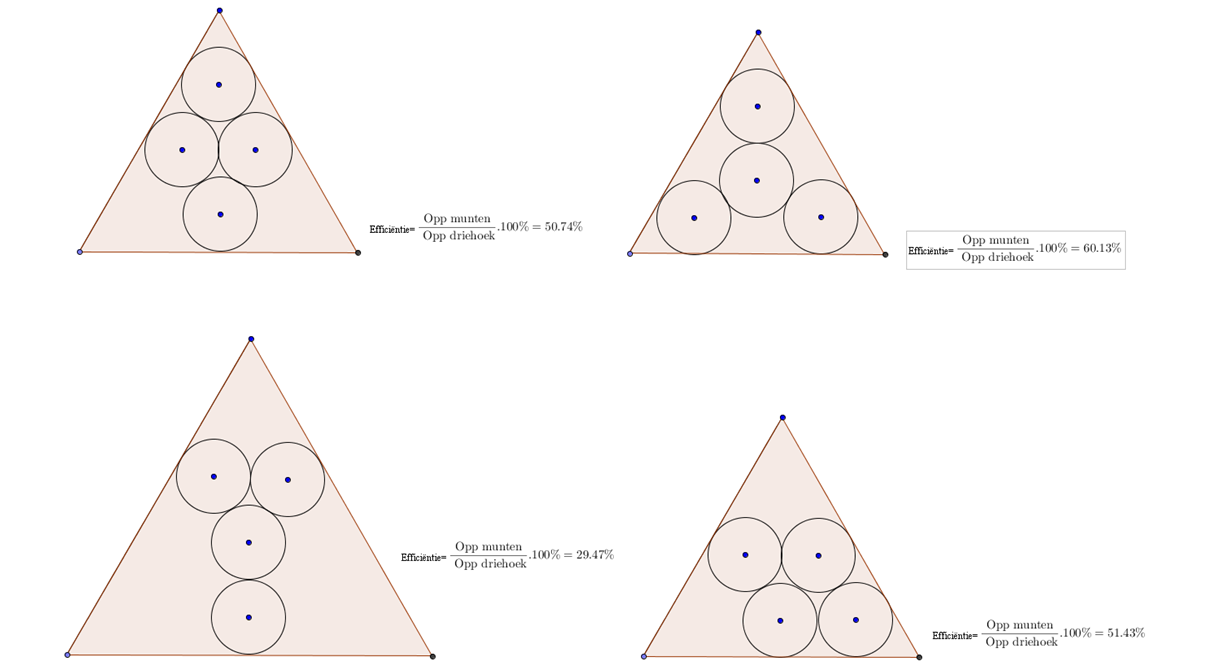
\includegraphics[height=4cm]{figuur4munten}
 % \caption{Configuraties met 4 munten in een driehoekig dienblad, die je niet verder kunt duwen, met verschillende effici�nties.}  
%\end{figure}
%\end{frame}



%\begin{frame}
%\frametitle{Tweedimensionale stapelproblemen}
%\framesubtitle{Dienbladenprobleem}

%\begin{block}{Vraag}
%Welke configuratie is de meest effici�nte?
%\end{block}
%\pause
%\begin{figure}[ht]
 % \centering
  %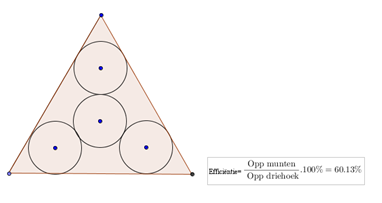
\includegraphics[height=3cm]{fig2}
  %\caption{Meest effici�nte configuratie met 4 munten in een driehoekig dienblad.}
  %\label{fig:efficientsteconfig}
%\end{figure}
%\pause
%\begin{block}{Opdracht}
%Bewijs dit!
%\end{block}


%\end{frame}


\begin{frame}
\frametitle{Les 6: Het dienbladenprobleem {\small (vervolg)}}
\framesubtitle{Didactische wenken}

\begin{enumerate}
	\item Onderwijsleergesprek
	\begin{itemize}
	\item Doel van deze les en de opdracht laten aanvoelen en uitleggen
\end{itemize}
	
	\item In groepjes werken
	\begin{itemize}
	\item A.d.h.v. een bundeltje met vragen en opdrachten iets bewijzen waarbij ze het stappenplan kunnen volgen
	\item M.b.v. een (zelfgemaakte) figuur het bewijs visueel maken
	\item Experimenteren, tekenen en berekenen
	% Leerkracht helpt waar nodig en loopt rond!!
\end{itemize}

  \item Onderwijsleergesprek
  \begin{itemize}
  \item Moeilijkheden en problemen in het bewijs samen overlopen
  \item Eventueel nog enkele ingewikkeldere configuraties berekenen
	\item Resultaten in de tabel samenleggen.
\end{itemize}

  \item Klasgesprek
  \begin{itemize}
	  \item Opmerkelijke zaken bespreken
	  \item Conclusies trekken
  \end{itemize}
\end{enumerate}
\end{frame}



\begin{frame}
\frametitle{Tweedimensionale stapelproblemen}
\framesubtitle{Dienbladenprobleem: Conclusie}



\begin{table}[h]
\centering
\small
\begin{tabular}{l||c|c|c|c}
Aantal / vorm & cirkelvormig & driehoekig & rechthoekig& zeshoekig\\\hline\hline
1&  100\% & 60,46\% & 78,54\%&90,69\%\\\hline
2& 50\%& 48,60\% & 78,54\%& 52,09\% \\\hline
3&64,62\%& 72,90\%  & 78,54\%& 68,02\%\\\hline
4&67,13\%&60,46\%&78,54\%&66,93\%\\\hline
5&68,52\%& 65,11\%  & 78,54\%& 62,14\%\\\hline
6&67,13\%&77,41\%&78,54\%&65,10\%\\\hline
7&77,78\%& 63,71\%  & 78,54\%& 85,05\%\\\hline
8&72,42\%&64,02\%&78,54\%&69,03\%\\\hline
9&67,57\%&72,02\%&78,54\%&66,03\%\\\hline
10&66,94\%&79,06\%&78,54\%& 71,13\%\\\hline
11&71,45\%& 64,40\%  & 79,06\%& 64,79 \%\\\hline
12&73,58\%&65,75\%&78,54\%&75,99\%\\\hline
13&72,45\%& 71,77 \%  & 78,54\%& 70,20 \%
\end{tabular}
\caption{\scriptsize De effici�ntie van de dienbladen bij een bepaalde hoeveelheid glazen of blikjes.}
\label{}
\end{table}



\end{frame}


\begin{frame}
\frametitle{Tweedimensionale stapelproblemen}
\framesubtitle{Dienbladenprobleem: Conclusie}



\begin{table}[h]
\centering
\small
\begin{tabular}{l||c|c|c|c}
Aantal / vorm & cirkelvormig & driehoekig & rechthoekig& zeshoekig\\\hline\hline
1& \cellcolor[rgb]{0.6,0.6,0.6} 100\% & 60,46\% & 78,54\%&90,69\%\\\hline
2& 50\%& 48,60\% & \cellcolor[rgb]{0.6,0.6,0.6}78,54\%& 52,09\% \\\hline
3&64,62\%& 72,90\% \cellcolor[rgb]{0.6,0.6,0.6} & 78,54\%& 68,02\%\\\hline
4&67,13\%&60,46\%&\cellcolor[rgb]{0.6,0.6,0.6}78,54\%&66,93\%\\\hline
5&68,52\%& 65,11\%  &\cellcolor[rgb]{0.6,0.6,0.6} 78,54\%& 62,14\%\\\hline
6&67,13\%&77,41\%&\cellcolor[rgb]{0.6,0.6,0.6}78,54\%&65,10\%\\\hline
7&77,78\%& 63,71\%  & 78,54\%& \cellcolor[rgb]{0.6,0.6,0.6} 85,05\%\\\hline
8&72,42\%&64,02\%&\cellcolor[rgb]{0.6,0.6,0.6}78,54\%&69,03\%\\\hline
9&67,57\%&72,02\%&\cellcolor[rgb]{0.6,0.6,0.6}78,54\%&66,03\%\\\hline
10&66,94\%&\cellcolor[rgb]{0.6,0.6,0.6}79,06&78,54\%& 71,13\%\\\hline
11&71,45\%& 64,40\%  & \cellcolor[rgb]{0.6,0.6,0.6}79,06\%& 64,79 \%\\\hline
12&73,58\%&65,75\%&\cellcolor[rgb]{0.6,0.6,0.6}78,54\%&75,99\%\\\hline
13&72,45\%& 71,77 \%  &\cellcolor[rgb]{0.6,0.6,0.6} 78,54\%& 70,20 \%
\end{tabular}
\caption{\scriptsize De effici�ntie van de dienbladen bij een bepaalde hoeveelheid glazen of blikjes.}
\label{}
\end{table}



\end{frame}


\subsection{Les 7: Kanonskogels stapelen}
\begin{frame}
\frametitle{Les 7: Kanonskogels stapelen}
\framesubtitle{Overzicht van de lessen}
\begin{list}{\quad}{}
\item Les 1: Inleiding
\item Les 2: Vullen van vierkanten met kleinere vierkanten en zo tot Perfecte Vierkanten komen
\item Les 3: Puzzelen met vierkanten en rechthoeken om vergelijkingen op te lossen
\item Les 4: Kennismaking met tweedimensionale stapelproblemen en het dienbladenprobleem 
\item Les 5: Het dienbladenprobleem: experimenteren en effectief berekenen
\item Les 6: Het dienbladenprobleem: berekenen, bewijzen en besluiten
\item {\color{blue}Les 7: Kanonskogels stapelen}
\item Les 8: Vervolg kanonskogels en het bolstapelprobleem van Kepler
\end{list}
\end{frame}

\begin{frame}
\frametitle{Les 7: Kanonskogels stapelen}
\framesubtitle{Lesdoelstellingen}
\begin{itemize}
\item De leerlingen weten wat het \textbf{bolstapelprobleem} inhoudt.
\item De leerlingen kunnen het \textbf{aantal kanonskogels in een (regelmatige) piramide} met vierkant en driehoekig grondvlak met $n$ lagen experimenteel berekenen.
\item De leerlingen kunnen vanuit een gegeven \textbf{rij} het recursief en/of expliciet \textbf{voorschrift} geven.
\item De leerlingen kunnen door het \textbf{doordacht experimenteren} bepaalde vragen over combinaties van piramides onderzoeken.
\item De leeringen kunnen een bewijs geven voor de \textbf{som van de eerste $n$ kwadraten}.
\item De leerlingen kunnen op een analoge wijze het bewijs geven voor de \textbf{som van de eerst $n$ driehoeksgetallen}.
\end{itemize}
\end{frame}

\begin{frame}
\frametitle{Les 7: Kanonskogels stapelen}
\framesubtitle{Didactische wenken}
\begin{enumerate}
	\item Onderwijsleergesprek
	\begin{itemize}
	\item Algemene inleding geven van het bolstapelprobleem, i.h.b. over het stapelen van kanonskogels	
\end{itemize}
  \item In groepjes werken en experimenteren
  \begin{itemize}
	\item Het aantal kanonskogels in een regelmatige piramide met vierkant en driehoekig grondvlak bepalen
	\item Vanuit de gegevens een formule proberen opstellen
	\item Complexere vragen i.v.m. het combineren van bepaalde stapels onderzoeken
\end{itemize}
  \item Onderwijsleergesprek
  \begin{itemize}
	  \item Overlopen wat de leerlingen hebben ontdekt
	  \item De expliciete formule voor \textquoteleft het aantal kogels' bepalen en bewijzen
	  \begin{itemize}
	\item De som van de eerste $n$ kwadraten
	\item De som van de eerste $n$ driehoeksgetallen
\end{itemize}
  \end{itemize}
  
\end{enumerate}

\end{frame}
\begin{frame}
\frametitle{Driedimensionale stapelproblemen}
\framesubtitle{Kanonskogels stapelen: aantal bepalen}

\begin{itemize}
	\item Het aantal kanonskogels bij een piramide met vierkant grondvlak: \begin{align*} v(n)&= 1^2 + 2^2 + \cdots + n^2= \sum_{i=1}^{n}i^2\\ &= \frac{1}{3}n^3+\frac{1}{2}n^2+\frac{1}{6}n .\end{align*}
	\item Het aantal kanonksogels bij een piramide met driehoekig grondvlak: \begin{align*} d(n) &= \frac{1.2}{2} + \frac{2.3}{2}+\frac{3.4}{2} + \cdots + \frac{n(n+1)}{2}=\sum_{i=1}^{n}\frac{i(i+1)}{2}\\ 
&=\frac{1}{6}n^3 + \frac{1}{2}n^2+\frac{1}{3}n.
\end{align*}
\end{itemize}

\end{frame}


\subsection{Les 8: Vervolg kanonskogels en het bolstapelprobleem van Kepler}
\begin{frame}
\frametitle{Les 8: Kanonskogels stapelen {\small (vervolg)}}
\framesubtitle{Overzicht van de lessen}
\begin{list}{\quad}{}
\item Les 1: Inleiding
\item Les 2: Vullen van vierkanten met kleinere vierkanten en zo tot Perfecte Vierkanten komen
\item Les 3: Puzzelen met vierkanten en rechthoeken om vergelijkingen op te lossen
\item Les 4: Kennismaking met tweedimensionale stapelproblemen en het dienbladenprobleem 
\item Les 5: Het dienbladenprobleem: experimenteren en effectief berekenen
\item Les 6: Het dienbladenprobleem: berekenen, bewijzen en besluiten
\item Les 7: Kanonskogels stapelen
\item {\color{blue}Les 8: Vervolg kanonskogels en het bolstapelprobleem van Kepler}
\end{list}
\end{frame}

\begin{frame}
\frametitle{Les 8: Kanonskogels stapelen {\small (vervolg)}}
\framesubtitle{Lesdoelstellingen}
\begin{itemize}
\item De leerlingen kunnen door het \textbf{doordacht experimenteren} bepaalde vragen over combinaties van piramides onderzoeken.
\item De leerlingen kunnen vanuit een voorbeeld komen tot een \textbf{algemene formule} en dit ook bewijzen, al dan niet met behulp van de leerkracht.
\item De leerlingen weten wat het \textbf{bolstapelprobleem} inhoudt.
\item De leerlingen weten wat een \textquoteleft \textbf{kissing number}' is.
\item De leerlingen \textbf{beseffen} dat het vinden van een bewijs soms vele jaren kan duren.
\item De leerlingen beseffen dat de controle van een bewijs soms geen evidentie is, bijvoorbeeld omdat een deel van het bewijs door een \textbf{computerprogramma} geleverd wordt.

\end{itemize}
\end{frame}

\begin{frame}
\frametitle{Les 8: Kanonskogels stapelen {\small (vervolg)}}
\framesubtitle{Didactische wenken}

\begin{enumerate}
	\item Onderwijsleergesprek
	\begin{itemize}
	\item Algemene bevindingen vorige les overlopen
	\item (Enkele) vermoedens i.v.m. de vragen over combinaties ook bewijzen
\end{itemize}
	\item{Quiz}
	\begin{itemize}
	\item Meerkeuzevragen in teams tegen elkaar
	\item A.d.h.v. de vragen en antwoorden op een speelse wijze het ontstaan, de evolutie en het bewijs van het \textquoteleft bolstapelprobleem van Kepler' vertellen
	\item Leerlingen laten stilstaan bij belangrijke fases in de zoektocht naar een bewijs
\end{itemize}
\end{enumerate}

\end{frame}

%
\begin{frame}
\frametitle{Driedimensionale stapelproblemen}
\framesubtitle{Kanonskogels stapelen: combinaties van stapels}

\begin{block}{Vraag:Is nu mogelijk om van een driehoekige stapel van een bepaalde hoogte een vierkante piramide te maken, zonder dat je kogels overhoudt?}
Neen, zie Frist Beukers en Jaap Top (1982).
\end{block}

\begin{block}{Vraag: Kan je van twee stapels knikkers in driehoekige piramides een nieuwe vierkante piramide maken?}
Ja, want \[d(n-1)-d(n)=v(n).\]
\end{block}

\begin{block}{Vraag: Kan je van een combinatie van een driehoekige en vierkante piramides een andere combinatie van een driehoekige en vierkante piramide maken?}
Ja, want \[ v(n)+d(n+1)= d(n-1) + v(n+1).\]
\end{block}
\end{frame}


\frame{
%\begin{figure}[t]
%	\flushleft
%		\includegraphics[scale=0.1]{logo.jpg}
%\end{figure}

\begin{block}
{\begin{center} Quiz: Bolstapelprobleem van Kepler \end{center}}
\end{block}

\begin{figure}[h]
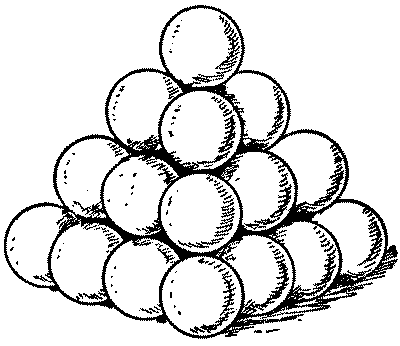
\includegraphics[width=4cm]{cannonballs}
\end{figure}
}
\section{Ontstaan}
\subsection{Vraag 1}
\begin{frame}

\begin{block}
{Wie was de wetenschappelijk adviseur van Sir Walter Raleigh?}

\begin{itemize}
	\item[A] Thomas Harriot
	\item[B] Johannes Kepler
	\item[C] Hij had geen wetenschappelijk adviseur
\end{itemize}
\end{block}

\begin{figure}
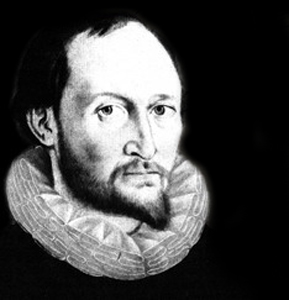
\includegraphics[height=3cm]{harriot}
\end{figure}


\end{frame}

\begin{frame}

\begin{block}
{Wie was de wetenschappelijk adviseur van Sir Walter Raleigh?}

\begin{itemize}
	\item[\textbf{A}] \textbf{Thomas Harriot}
	\item[B] Johannes Kepler
	\item[C] Hij had geen wetenschappelijk adviseur
\end{itemize}
\end{block}

\begin{figure}
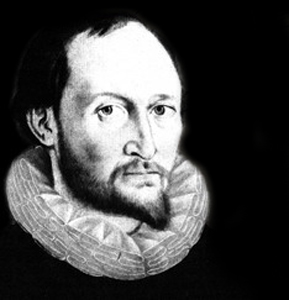
\includegraphics[height=3cm]{harriot}
\end{figure}


\end{frame}

\subsection{Vraag 2}

\begin{frame}

\begin{block}
{Wat is de nationaliteit van Johannes Kepler?}

\begin{itemize}
	\item[A] Duitser
	\item[B] Oostenrijker
	\item[C] Engelsman
	\end{itemize}
\end{block}
\begin{figure}[h]
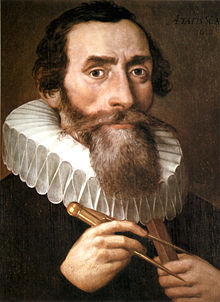
\includegraphics[heigth=5cm]{kepler}

\end{figure}

\end{frame}


\begin{frame}

\begin{block}
{Wat is de nationaliteit van Johannes Kepler?}

\begin{itemize}
	\item[\textbf{A}] \textbf{Duitser}
	\item[B] Oostenrijker
	\item[C] Engelsman
	\end{itemize}
\end{block}
\begin{figure}[h]
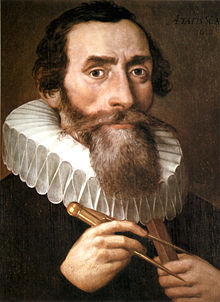
\includegraphics[heigth=5cm]{kepler}

\end{figure}

\end{frame}


\subsection{Vraag 3}
\begin{frame}

\begin{block}
{Welke term betekent niet 'het maximum aantal niet-overlappende eenheidssferen dat aan een gegeven eenheidssfeer raakt'?}

\begin{itemize}
	\item[A] Newton number
	\item[B] Kissing number
	\item[C] Contact number
	\item[D] Kepler number
	\end{itemize}
\end{block}

\begin{figure}[h]
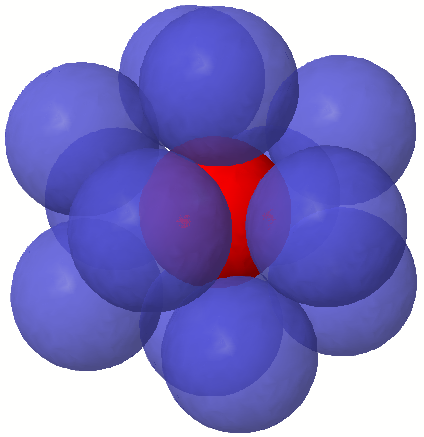
\includegraphics[width=3cm]{kissing}
\end{figure}
%D

\end{frame}

\begin{frame}

\begin{block}
{Welke term betekent niet 'het maximum aantal niet-overlappende eenheidssferen dat aan een gegeven eenheidssfeer raakt'?}

\begin{itemize}
	\item[A] Newton number
	\item[B] Kissing number
	\item[C] Contact number
	\item[\textbf{D}] \textbf{Keper number}
	\end{itemize}
\end{block}

\begin{figure}[h]
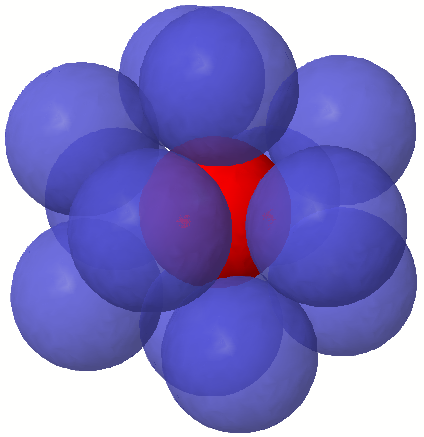
\includegraphics[width=3cm]{kissing}
\end{figure}
%D

\end{frame}


\section{Evolutie}
\subsection{Vraag 4}

\begin{frame}

\begin{block}{Welke Duitse Wiskundige bewees dat de \textquoteleft face-centered cubic packing' de dichtste pakkingsmethode is volgens een rooster?}
\begin{itemize}
	\item[A] Kepler
	\item[B] Gauss
	\item[C] Hilbert 
\end{itemize}
\end{block}

\begin{figure}[h]
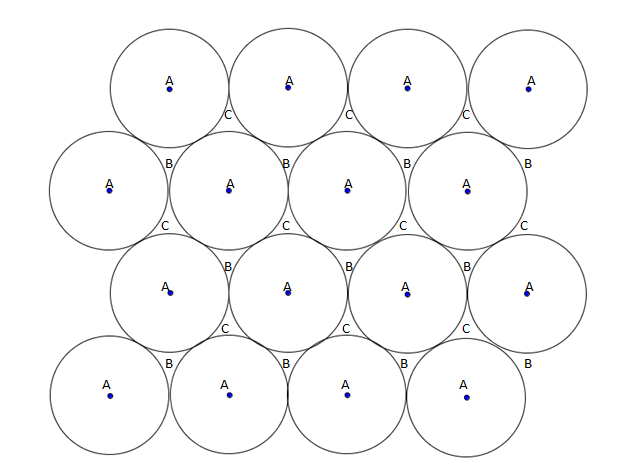
\includegraphics[height=3cm]{fcc}
\end{figure}
\end{frame}

\begin{frame}

\begin{block}{Welke Duitse Wiskundige bewees dat de \textquoteleft face-centered cubic packing' de dichtste pakkingsmethode is volgens een rooster?}
\begin{itemize}
	\item[A] Kepler
	\item[\textbf{B}] \textbf{Gauss}
	\item[C] Hilbert 
\end{itemize}
\end{block}

\begin{figure}[h]
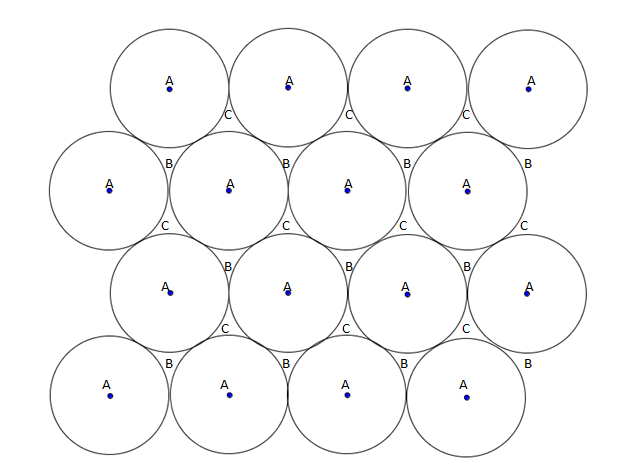
\includegraphics[height=3cm]{fcc}
\end{figure}
\end{frame}


\subsection{Vraag 5}

\begin{frame}
\begin{block}
{Welke Scandinavische wiskundige ontwikkelde een theorie over het tweedimensionale equivalent voor 'het probleem van Kepler' waarin men zicht naar de dichtste pakkingsmethode voor cirkels in het vlak?}
\begin{itemize}
	\item[A] Axel Thue
	\item[B] L�szlo Feje T�th
	\item[C] Wu-Yi Hsiang
	\end{itemize}
\end{block}
\begin{figure}[h]
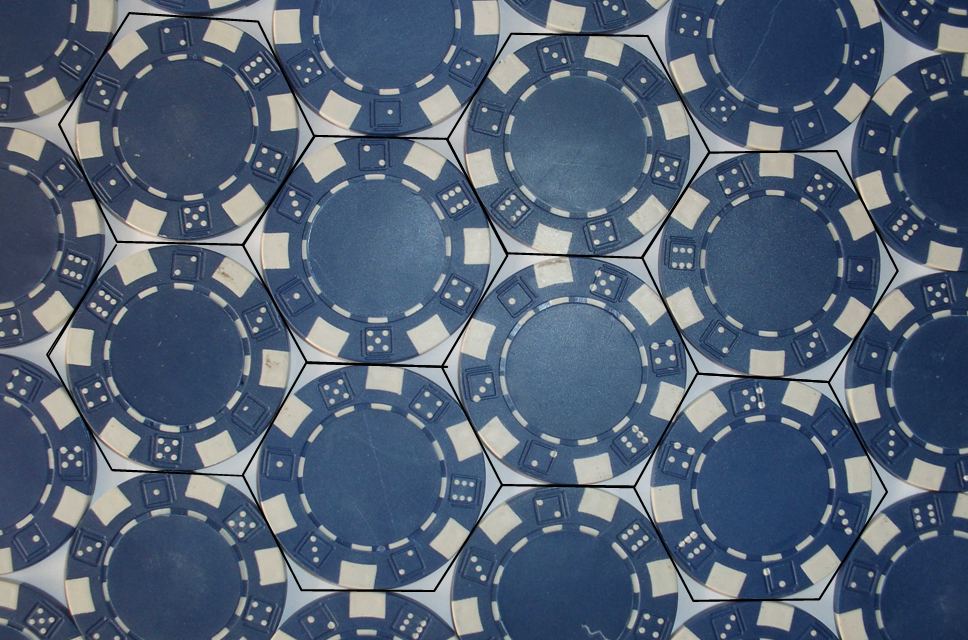
\includegraphics[width=3cm]{voronoi_hex}
\end{figure}
\end{frame}

\begin{frame}
\begin{block}
{Welke Scandinavische wiskundige ontwikkelde een theorie over het tweedimensionale equivalent voor 'het probleem van Kepler' waarin men zicht naar de dichtste pakkingsmethode voor cirkels in het vlak?}

\begin{itemize}
	\item[\textbf{A}] \textbf{Axel Thue}
	\item[B] L�szlo Feje T�th
	\item[C] Wu-Yi Hsiang
	\end{itemize}
\end{block}

\begin{figure}[h]
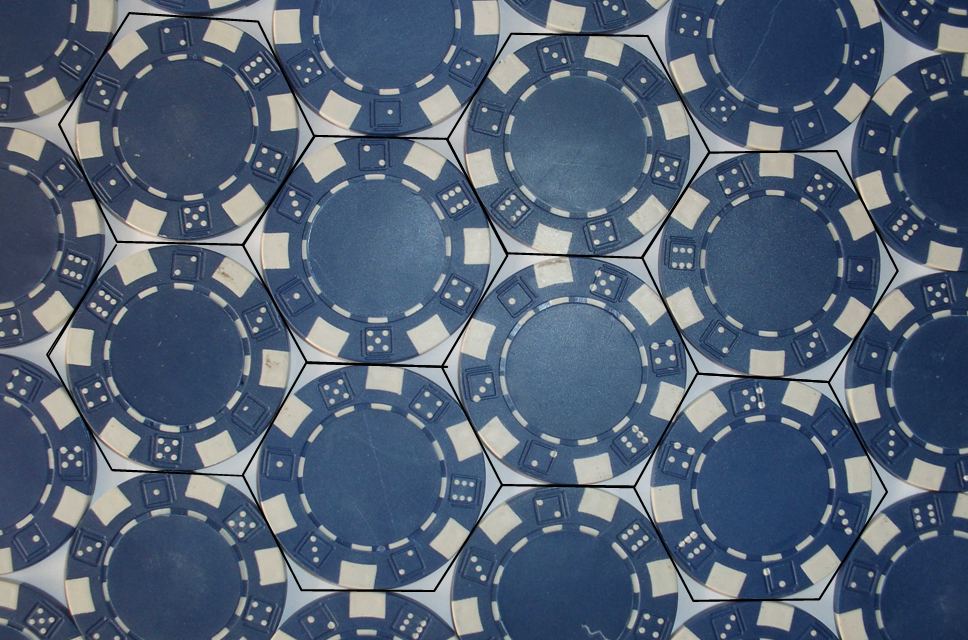
\includegraphics[width=3cm]{voronoi_hex}
\end{figure}

\end{frame}

\subsection{Vraag 6}

\begin{frame}
\begin{block}
{Kepler vermoedde dat de dichtheid van de dichtste bolstapeling $\frac{\pi}{\sqrt{18}}$ is. Wat is deze effici�ntie als percentage?}

\begin{itemize}
	\item[A] 74,0480 \%
	\item[B] 77,964 \%
	\item[C] 77,844 \%
	\item[D] 77,3055 \%
	\end{itemize}
\end{block}


\end{frame}


\begin{frame}
\begin{block}
{Kepler vermoedde dat de dichtheid van de dichtste bolstapeling $\frac{\pi}{\sqrt{18}}$ is. Wat is deze effici�ntie als percentage?}

\begin{itemize}
	\item[\textbf{A}] \textbf{74,0480 \%}
	\item[B] 77,964 \%
	\item[C] 77,844 \%
	\item[D] 77,3055 \%
	\end{itemize}
\end{block}

\end{frame}
\section{Bewijs}
\subsection{Vraag 7}

\begin{frame}
\begin{block}
{Voor hoeveel stapelingen moest Thomas Hales uiteindelijk het probleem van Kepler aantonen?}

\begin{itemize}
	\item[A] 5
	\item[B] 50
	\item[C] 500
	\item[D] 5000
	\end{itemize}
\end{block}

\begin{figure}[h]
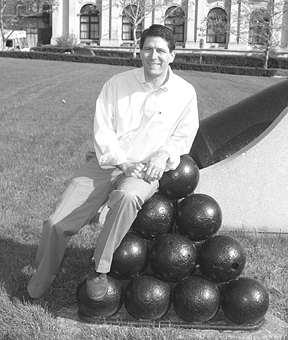
\includegraphics[width=3cm]{hales}
\end{figure}

\end{frame}


\begin{frame}
\begin{block}
{Voor hoeveel stapelingen moest Thomas Hales uiteindelijk het probleem van Kepler aantonen?}

\begin{itemize}
	\item[A] 5
	\item[B] 50
	\item[C] 500
	\item[\textbf{D}] \textbf{5000}
	\end{itemize}
\end{block}

\begin{figure}[h]
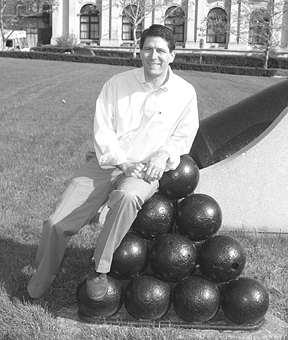
\includegraphics[width=3cm]{hales}
\end{figure}

\end{frame}

\subsection{Vraag 8}

\begin{frame}
\begin{block}
{Waarom bleken er voor sommigen achteraf nog twijfels over het bewijs van Hales ?}

\begin{itemize}
	\item[A] Eigenlijk was het zijn assistent Samuel Ferguson die het bewijs had geleverd.
	\item[B] Het bewijs is zo lang dat het niet gecontroleerd kan worden.
	\item[C] Hales bewees de stelling met de computer.
	\end{itemize}
\end{block}

\begin{figure}[h]
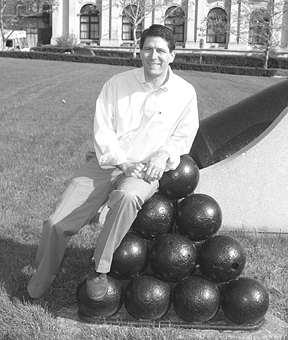
\includegraphics[width=3cm]{hales}
\end{figure}

\end{frame}


\begin{frame}
\begin{block}
{Waarom bleken er voor sommigen achteraf nog twijfels over het bewijs van Hales ?}

\begin{itemize}
	\item[A] Eigenlijk was het zijn assistent Samuel Ferguson die het bewijs had geleverd.
	\item[B] Het bewijs is zo lang dat het niet gecontroleerd kan worden.
	\item[\textbf{C}] \textbf{Hales bewees de stelling met de computer.}
	\end{itemize}
\end{block}

\begin{figure}[h]
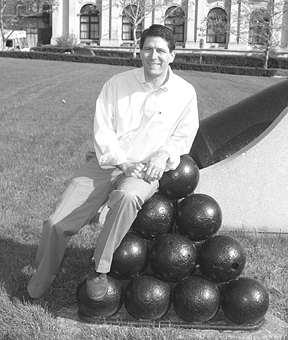
\includegraphics[width=3cm]{hales}
\end{figure}

\end{frame}



\section{Wijzigingen aanbrengen}

\begin{frame}
  \frametitle{Wijzigingen aanbrengen}
%  \framesubtitle{}
  Website: \url{http://wiskunde.github.com/V3/}\\
  \vspace*{0.5cm}
  \begin{columns}[t]
    \begin{column}{0.5\textwidth}
      Samenwerking gebaseerd op:
      \begin{itemize}
        \item Overleg\\
          \visible<2->{
          \begin{itemize}
            \item Vergaderen
            \item Email
          \end{itemize}
          }
        \item \LaTeX\\
          \visible<3->{
          \begin{itemize}
            \item Fantastische typesetting!
            \item Simpele tekstbestanden
            \item \href{http://www.tug.org/twg/mactex/tutorials/ltxprimer-1.0.pdf}{Boek}
          \end{itemize}
          }
        \item Git\\
          \visible<4->{
          \begin{itemize}
            \item Versiecontrole systeem
            \item Elk heeft eigen versie
            \item Samen versie online
            \item \href{http://git-scm.com/book}{Boek}
          \end{itemize}
          }
      \end{itemize}
    \end{column}
    \begin{column}{0.5\textwidth}
      \visible<5->{
        Voordelen voor leerkrachten:
        \begin{itemize}
          \item Eigen versie:
          \visible<6->{
            \begin{itemize}
              \item Huisstijl
              \item Herschikken materiaal
              \item Materiaal naar keuze
              \item Inpassen in eigen lessen
            \end{itemize}
          }
          \item Versie online:
          \visible<7->{
            \begin{itemize}
              \item Verbeteren materiaal
              \item Toevoegen materiaal
              \item Didactiek verbeteren
            \end{itemize}
          }
        \end{itemize}
      }
    \end{column}
  \end{columns}
\end{frame}


\begin{frame}
{Overzicht van de lessen}
\begin{list}{\quad}{}
\item Les 1: Inleiding
\item Les 2: Vullen van vierkanten met kleinere vierkanten en zo tot Perfecte Vierkanten komen
\item Les 3: Puzzelen met vierkanten en rechthoeken om vergelijkingen op te lossen
\item Les 4: Kennismaking met tweedimensionale stapelproblemen en het dienbladenprobleem 
\item Les 5: Het dienbladenprobleem: experimenteren en effectief berekenen
\item Les 6: Het dienbladenprobleem: berekenen, bewijzen en besluiten
\item Les 7: Kanonskogels stapelen
\item Les 8: Vervolg kanonskogels en het bolstapelprobleem van Kepler
\end{list}
\end{frame}

\end{document}
